\documentclass[12pt,a4paper,oneside,openany]{book}

% Configuración general y datos editables del documento.
% =============================================================================
% Configuración general del documento
% =============================================================================

% Idioma, codificación y tipografía
\usepackage[utf8]{inputenc}
\usepackage[T1]{fontenc}
\usepackage[provide=*,spanish]{babel}
\AtBeginDocument{\ifdefined\decimalpoint\decimalpoint\fi}
\usepackage{lmodern}

% Página y composición tipográfica
\usepackage[
  a4paper,
  top=2.8cm,
  bottom=2.8cm,
  left=3.2cm,
  right=2.8cm,
  headheight=14.5pt
]{geometry}
\usepackage{microtype}
\usepackage{setspace}
\onehalfspacing
\setlength{\parindent}{1.25cm}
\setlength{\parskip}{0pt}
\setlength{\emergencystretch}{2em}
\raggedbottom

% Matemáticas y unidades
\usepackage{amsmath,amssymb,mathtools}

% Figuras y tablas
\usepackage{graphicx}
\graphicspath{{Figuras/}}
\usepackage{booktabs}
\usepackage{longtable}
\usepackage{tabularx}
\usepackage{array}
\usepackage{multirow}
\usepackage{caption}
\usepackage{subcaption}
\usepackage{float}
\usepackage{placeins}
\captionsetup{font=small,labelfont=bf}

% Listas y código fuente
\usepackage{enumitem}
\usepackage{listings}
\usepackage{xcolor}
\definecolor{codigoFondo}{RGB}{247,248,250}
\definecolor{codigoComentario}{RGB}{75,120,75}
\lstset{
  basicstyle=\ttfamily\small,
  backgroundcolor=\color{codigoFondo},
  commentstyle=\color{codigoComentario},
  frame=single,
  breaklines=true,
  showstringspaces=false,
  tabsize=4
}

% Títulos de capítulos y secciones
\usepackage{titlesec}
\titleformat{\chapter}[hang]
  {\normalfont\bfseries\Large}
  {\thechapter.}
  {0.75em}
  {}
\titleformat{name=\chapter,numberless}[hang]
  {\normalfont\bfseries\Large}
  {}
  {0pt}
  {}
\titlespacing*{\chapter}{0pt}{0pt}{1.6em}
\titlespacing*{\section}{0pt}{2.2ex plus 0.5ex minus 0.2ex}{1.0ex}
\titlespacing*{\subsection}{0pt}{2.0ex plus 0.5ex minus 0.2ex}{0.8ex}
\setcounter{secnumdepth}{3}
\setcounter{tocdepth}{3}

% Encabezados y pies de página
\usepackage{fancyhdr}
\fancypagestyle{plain}{%
  \fancyhf{}
  \fancyfoot[C]{\thepage}
  \renewcommand{\headrulewidth}{0pt}
  \renewcommand{\footrulewidth}{0pt}
}

% Citas y referencias. En Overleaf se emplea biblatex-apa con Biber.
% El segundo bloque permite compilar en instalaciones mínimas de LaTeX.
\usepackage{csquotes}
\IfFileExists{biblatex.sty}{%
  \usepackage[
    backend=biber,
    style=apa,
    sorting=nyt,
    sortcites=true,
    maxbibnames=99,
    giveninits=true,
    uniquename=false
  ]{biblatex}
  \DeclareLanguageMapping{spanish}{spanish-apa}
  \addbibresource{referencias.bib}
  \newcommand{\imprimirreferencias}{%
    \cleardoublepage
    \printbibliography[heading=bibintoc,title={Referencias}]%
  }
}{%
  \usepackage[authoryear,round]{natbib}
  \bibliographystyle{apalike}
  \providecommand{\parencite}[1]{\citep{#1}}
  \providecommand{\textcite}[1]{\citet{#1}}
  \newcommand{\imprimirreferencias}{%
    \cleardoublepage
    \phantomsection
    \addcontentsline{toc}{chapter}{Referencias}
    \bibliography{referencias}%
  }
}


% Figuras y algoritmos para el desarrollo metodológico.
\usepackage{svg}
\svgpath{{Figuras/}}
\newcommand{\FiguraMetodologia}[2]{%
  \includegraphics[width=#1]{Figuras/#2.pdf}%
}
\usepackage{algorithm}
\usepackage{algpseudocode}
\numberwithin{algorithm}{chapter}
\floatname{algorithm}{Algoritmo}
\algrenewcommand\algorithmicrequire{\textbf{Entrada:}}
\algrenewcommand\algorithmicensure{\textbf{Salida:}}
\algrenewcommand\algorithmicif{\textbf{si}}
\algrenewcommand\algorithmicthen{\textbf{entonces}}
\algrenewcommand\algorithmicelse{\textbf{en otro caso}}
\algrenewcommand\algorithmicfor{\textbf{para}}
\algrenewcommand\algorithmicdo{\textbf{hacer}}
\algrenewcommand\algorithmicend{\textbf{fin}}
\algrenewcommand\algorithmicreturn{\textbf{devolver}}
\algrenewcommand\algorithmicfunction{\textbf{función}}

% Hipervínculos y referencias cruzadas: deben cargarse al final.
\usepackage[hidelinks]{hyperref}
\usepackage{bookmark}
\usepackage[capitalise,noabbrev]{cleveref}
\hypersetup{
  pdftitle={Reconstrucción muográfica por transmisión asistida por aprendizaje profundo mediante mejora predictiva de imágenes de baja estadística para exploración volcánica},
  pdfauthor={Reinaldo Cárdenas Tirado y Daniel Andrés Pinto Ortega},
  pdfsubject={Trabajo de grado - Ingeniería de Sistemas - GOTS},
  pdfkeywords={muografía, exploración volcánica, Geant4, EcoMug, aprendizaje profundo}
}

% Nombres en español
\addto\captionsspanish{%
  \renewcommand{\contentsname}{Índice general}
  \renewcommand{\tablename}{Tabla}
  \renewcommand{\listtablename}{Índice de tablas}
  \renewcommand{\listfigurename}{Índice de figuras}
  \renewcommand{\bibname}{Referencias}
}
\crefname{figure}{figura}{figuras}
\Crefname{figure}{Figura}{Figuras}
\crefname{table}{tabla}{tablas}
\Crefname{table}{Tabla}{Tablas}
\crefname{section}{sección}{secciones}
\Crefname{section}{Sección}{Secciones}
\crefname{chapter}{capítulo}{capítulos}
\Crefname{chapter}{Capítulo}{Capítulos}
\crefname{equation}{ecuación}{ecuaciones}
\Crefname{equation}{Ecuación}{Ecuaciones}

% Comandos útiles del proyecto
\newcommand{\ContenidoPendiente}{%
  \par\noindent
  {\small\color{gray}\textit{Contenido pendiente de incorporación y revisión.}}%
  \par\vspace{0.45\baselineskip}
}

% El logotipo PDF tiene prioridad. El JPG permite que este paquete compile
% inmediatamente y puede eliminarse cuando se copie Figuras/logo_uis.pdf.
\newcommand{\LogoUIS}[1][0.23\textwidth]{%
  \IfFileExists{Figuras/logo_uis.pdf}{%
    
\includegraphics[width=#1]{Figuras/logo_uis.pdf}%
  }{%
    \IfFileExists{Figuras/logo_uis.jpg}{%
      \includegraphics[width=#1]{Figuras/logo_uis.jpg}%
    }{%
      \fbox{\parbox[c][2.1cm][c]{4.2cm}{\centering Logo UIS\\pendiente}}%
    }%
  }%
}

\makeatletter\def\theHALG@line{\thealgorithm.\arabic{ALG@line}}\makeatother

% Esqueleto de trabajo: estas guías son editoriales, no texto final de la tesis.
% Cambiar a \mostrarGuiasfalse cuando se desee ocultarlas en el PDF.
\newif\ifmostrarGuias
\mostrarGuiastrue
\newcommand{\GuiaRedaccion}[1]{%
  \ifmostrarGuias
    \par\noindent{\small\color{gray}\textit{Guía de redacción: #1}}\par
  \fi
}

% =============================================================================
% Datos editables del trabajo de grado
% =============================================================================

\newcommand{\TituloTrabajo}{Reconstrucción muográfica por transmisión asistida por aprendizaje profundo mediante mejora predictiva de imágenes de baja estadística para exploración volcánica}

\newcommand{\AutorUno}{Reinaldo Cárdenas Tirado}
\newcommand{\CodigoAutorUno}{2190201}
\newcommand{\AutorDos}{Daniel Andrés Pinto Ortega}
\newcommand{\CodigoAutorDos}{2190558}

\newcommand{\TipoDocumento}{Trabajo de grado, modalidad Trabajo de Investigación,}
\newcommand{\TituloObtenido}{Ingeniero de Sistemas}

\newcommand{\DirectorNombre}{Andrés Leonardo González Gómez}
\newcommand{\DirectorTitulo}{PhD(c).}
\newcommand{\DirectorFormacion}{Candidato a Doctor en Ciencias de la Computación}

\newcommand{\CodirectorNombre}{Jaime Enrique Meneses Fonseca}
\newcommand{\CodirectorTitulo}{PhD.}
\newcommand{\CodirectorFormacion}{Doctor en Ciencias para la Ingeniería}

\newcommand{\Universidad}{Universidad Industrial de Santander}
\newcommand{\Facultad}{Facultad de Ingenierías Fisicomecánicas}
\newcommand{\Escuela}{Escuela de Ingeniería de Sistemas e Informática}
\newcommand{\Programa}{Programa de Ingeniería de Sistemas}
\newcommand{\Ciudad}{Bucaramanga}
\newcommand{\AnioDocumento}{2026}

\newcommand{\BloqueInstitucional}{%
  {\Universidad\par}
  {\Facultad\par}
  {\Escuela\par}
  {\Programa\par}
  {\Ciudad\par}
  {\AnioDocumento\par}
}


\begin{document}

% -----------------------------------------------------------------------------
% Páginas iniciales sin numeración
% -----------------------------------------------------------------------------
\hypersetup{pageanchor=false}
\pagenumbering{gobble}
\pagestyle{empty}
\begin{titlepage}
  \centering
  \begin{spacing}{1.12}
    \vspace*{1.15cm}

    {\fontsize{16}{21}\selectfont\bfseries
      \MakeUppercase{\TituloTrabajo}\par}

    \vspace{2.25cm}

    {\large
      \AutorUno, \CodigoAutorUno\par
      \AutorDos, \CodigoAutorDos\par}

    \vspace{1.75cm}

    \LogoUIS[4.35cm]

    \vfill

    {\large\MakeUppercase{\BloqueInstitucional}}
  \end{spacing}
\end{titlepage}

\begin{titlepage}
  \centering
  \begin{spacing}{1.08}
    \vspace*{0.3cm}

    {\fontsize{14}{18}\selectfont\bfseries
      \MakeUppercase{\TituloTrabajo}\par}

    \vspace{1.0cm}

    {\large
      \TipoDocumento\par
      para optar al título de\par
      \textit{\TituloObtenido}\par}

    \vspace{0.75cm}

    {\large
      \textbf{Autores:}\par
      \AutorUno, \CodigoAutorUno\par
      \AutorDos, \CodigoAutorDos\par}

    \vspace{0.65cm}

    {\large
      \textbf{Director:}\par
      Profesor: \DirectorNombre, \DirectorTitulo\par
      \DirectorFormacion\par}

    \vspace{0.55cm}

    {\large
      \textbf{Codirector:}\par
      Profesor: \CodirectorNombre, \CodirectorTitulo\par
      \CodirectorFormacion\par}

    \vspace{0.8cm}

    \LogoUIS[3.5cm]

    \vfill

    {\large\MakeUppercase{\BloqueInstitucional}}
  \end{spacing}
\end{titlepage}

\hypersetup{pageanchor=true}

% Si se requieren, activar las líneas siguientes.
% % Reservado para una etapa posterior de redacción.

% % Reservado para una etapa posterior de redacción.


% -----------------------------------------------------------------------------
% Elementos preliminares con numeración romana
% -----------------------------------------------------------------------------
\frontmatter
\pagenumbering{Roman}
\pagestyle{plain}

\tableofcontents

\cleardoublepage
\phantomsection
\addcontentsline{toc}{chapter}{Índice de tablas}
\listoftables

\cleardoublepage
\phantomsection
\addcontentsline{toc}{chapter}{Índice de figuras}
\listoffigures

% Activar cuando la cantidad de siglas justifique una lista independiente.
% % Reservado para una etapa posterior de redacción.


\chapter*{Resumen}
\addcontentsline{toc}{chapter}{Resumen}
\label{pre:resumen}

\begingroup
\setstretch{1.1}
\setlength{\parindent}{0pt}
\setlength{\parskip}{0.7em}

\textbf{Título:} \TituloTrabajo\footnote{Trabajo de grado, modalidad Trabajo de Investigación.}

\textbf{Autores:} \AutorUno; \AutorDos.\footnote{\Facultad. \Escuela. Director: \DirectorNombre, \DirectorTitulo Codirector: \CodirectorNombre, \CodirectorTitulo}

\textbf{Palabras clave:} muografía por transmisión, exploración volcánica, aprendizaje profundo, simulación Monte Carlo, mejora de imágenes, baja estadística.

\textbf{Descripción:}

% Cifras tomadas de los capítulos 4 y 5 (evaluación final EF-01 con la corrección C2).
La muografía por transmisión permite estimar la distribución de densidad en el interior de un volcán a partir de la atenuación del flujo de muones cósmicos, pero el bajo flujo natural obliga a exposiciones de semanas o meses para que los contrastes de densidad se distingan del ruido de conteo. Este trabajo desarrolló y evaluó un esquema de mejora de imágenes muográficas de baja estadística basado en aprendizaje profundo y entrenado con datos sintéticos. Mediante simulación Monte Carlo con Geant4, con una fuente de muones derivada de una parametrización del flujo y del generador EcoMug, se obtuvieron 114 imágenes de referencia de diecinueve escenarios volcánicos idealizados y, por adelgazamiento binomial, 9\,120 pares de entrada y referencia con el 50, el 10, el 5 y el 1\,\% de los conteos, particionados por geometría. Con el 5\,\% de los conteos se diseñó, entrenó y evaluó una red generativa antagónica condicional de Wasserstein con penalización de gradiente, formada por un generador U-Net y un crítico PatchGAN, junto con una U-Net entrenada con pérdida L1 y variantes ajustadas para conservar las cuentas. En la evaluación final, descriptiva y sobre datos potencialmente expuestos, porque las escenas reservadas ya se habían evaluado antes, la red generativa aumentó en prueba el SSIM de 0,7643 a 0,8342 y el PSNR de 24,258 a 31,170~dB respecto de su entrada y, según ambas métricas, superó en cada una de las cuatro geometrías reservadas a la imagen sin procesar con el doble de conteos, aunque no a la obtenida con diez veces más. Al mismo tiempo, aumentó el sesgo regional de las cuentas de 1,832 a 14,566\,\%, y las variantes que lo redujeron disminuyeron la similitud. La calidad comparable a la de alta estadística quedó, por ello, respaldada solo de forma parcial, y el factor de reducción del tiempo de adquisición alcanzable no quedó demostrado: el valor nominal de 20 describe solo la reducción de conteos de la entrada. Los resultados se limitan a escenarios sintéticos idealizados y a una sola fracción de conteo; su extensión a datos de campo exige un criterio de calidad con un margen fundamentado y la respuesta de un detector físico.

\endgroup
 % Completar al finalizar los capítulos.
\chapter*{Abstract}
\addcontentsline{toc}{chapter}{Abstract}
\label{pre:abstract}

\begingroup
\setstretch{1.1}
\setlength{\parindent}{0pt}
\setlength{\parskip}{0.7em}

% Traducción de trabajo del título; revisar junto con el abstract definitivo.
\textbf{Title:} Deep learning-assisted transmission muographic reconstruction through predictive enhancement of low-statistics images for volcanic exploration.\footnote{Undergraduate thesis, research modality.}

\textbf{Authors:} \AutorUno; \AutorDos.\footnote{Universidad Industrial de Santander. Faculty of Physical and Mechanical Engineering. School of Systems Engineering and Informatics. Supervisor: \DirectorNombre, PhD candidate. Co-supervisor: \CodirectorNombre, PhD.}

\textbf{Keywords:} transmission muography, volcanic exploration, deep learning, Monte Carlo simulation, image enhancement, low statistics.

\textbf{Description:}

% Faithful translation of the Spanish description; keep both consistent.
Transmission muography estimates the density distribution inside a volcano from the attenuation of the cosmic-ray muon flux, but the low natural flux requires exposures of weeks or months before density contrasts can be distinguished from counting noise. This work investigated whether a deep learning model trained on synthetic data can transform low-statistics muographic images into images of quality comparable to high-statistics ones and thereby reduce the effective acquisition time in volcanic exploration. Monte Carlo simulations with Geant4 and EcoMug produced 114 references of nineteen idealized volcanic scenarios and, through binomial thinning, 9,120 input--reference pairs with 50, 10, 5 and 1\,\% of the counts, partitioned by geometry. With 5\,\% of the counts, a conditional Wasserstein generative adversarial network (cGAN), a U-Net baseline and six continuations with regional and boundary losses were trained and later evaluated at the four fractions. In a descriptive evaluation on potentially exposed data, the cGAN increased the test SSIM from 0.7643 to 0.8342 and the PSNR from 24.258 to 31.170~dB with respect to its input, below the U-Net, and outperformed on both metrics the unprocessed input with twice the counts in all twenty-four reserved views, but the regional count bias rose from 1.832 to 14.566\,\%. None of the 768 model--fraction--view combinations jointly reached the SSIM and PSNR of the unprocessed input at 50\,\%, so the reduction factor remained undetermined under that criterion. Local indicators, computed on anomalies of known location, showed simultaneous improvements and deteriorations and do not demonstrate the detection of unknown anomalies. It is concluded that the synthetic dataset fulfilled its objective, that comparable quality was only partially supported, and that neither an acquisition-time reduction factor nor quantitative opacity equivalence was demonstrated. The results are limited to synthetic scenarios, without a physical detector or field data.

\endgroup
 % Traducción fiel del resumen definitivo.

% -----------------------------------------------------------------------------
% Cuerpo principal con numeración arábiga
% -----------------------------------------------------------------------------
\mainmatter
\pagestyle{plain}

\chapter{Introducción}
\label{chap:introduccion}

% Versión 1 del capítulo 1 (2026-10-04). Base: plan de trabajo aprobado
% (introducción, planteamiento del problema, justificación y objetivos), redactado
% como informe y ajustado al alcance que sustentan los capítulos 3 a 5.

Conocer la distribución de densidad en el interior de un edificio volcánico es una de las bases de la evaluación de su amenaza. Los conductos por los que asciende el magma, las cavidades, las zonas de alteración hidrotermal y los cuerpos de roca más densa modifican la masa que hay a lo largo de cualquier trayecto que atraviese la montaña, y su localización ayuda a interpretar procesos como la desgasificación, el ascenso de material o la estabilidad de los flancos \parencite{tanaka2007asama,tanaka2023muography}. Los métodos geofísicos convencionales estiman esa estructura de forma indirecta, a partir de campos medidos en la superficie, y las técnicas de inspección por radiación artificial no alcanzan a atravesar cientos de metros de roca. Este trabajo se ocupa de una técnica que sí lo hace, la muografía por transmisión, y de una de sus limitaciones más severas: el tiempo de exposición que exige obtener una imagen interpretable.

\section{Contexto y planteamiento del problema}
\label{sec:intro-problema}

La muografía aprovecha los muones que se producen cuando los rayos cósmicos interactúan con la atmósfera. Por su energía elevada y su interacción débil con la materia, una fracción de esos muones atraviesa cientos de metros o incluso kilómetros de roca, y la atenuación de su flujo en cada dirección de observación indica cuánta materia hay a lo largo de ella \parencite{bonomi2020,tanaka2023muography}. Desde sus primeras aplicaciones volcánicas, la técnica ha permitido visualizar estructuras bajo el cráter del monte Asama \parencite{tanaka2007asama} y obtener imágenes de alta definición del volcán Sakurajima \parencite{olah2018sakurajima}, ambos en Japón. En Colombia se diseñó y construyó el telescopio híbrido MuTe con el propósito específico de estudiar volcanes activos del país en zonas de difícil acceso \parencite{penarodriguez2020}.

La fuente de la técnica es, al mismo tiempo, su principal limitación. A diferencia de la radiografía médica o industrial, en la que la intensidad de la fuente puede ajustarse, la muografía depende del flujo natural de muones, cercano a un muon por centímetro cuadrado y por minuto sobre un detector horizontal a nivel del mar \parencite{pdg2022}. En las direcciones casi horizontales con las que se observa un volcán ese flujo es mucho menor, y después de atravesar cientos de metros de roca solo sobrevive una fracción pequeña de él. El número de muones registrado en cada dirección es, por lo tanto, reducido y está sujeto a fluctuaciones aleatorias, de modo que se requieren exposiciones de semanas o meses para que los contrastes de densidad se distingan de esas fluctuaciones \parencite{lesparre2010}. Durante ese tiempo el instrumento debe operar en ambientes remotos, expuesto a la intemperie y con suministro de energía limitado, lo que encarece la adquisición, aumenta el riesgo de fallas y limita la frecuencia con la que puede actualizarse una imagen \parencite{bonomi2020,lechmann2021}. Las imágenes obtenidas con exposiciones cortas presentan un ruido de conteo elevado que puede enmascarar precisamente las estructuras que se pretende detectar.

En otros campos de la imagenología, el aprendizaje profundo ha ofrecido una alternativa al aumento del tiempo de adquisición. En la tomografía computarizada de baja dosis, por ejemplo, las redes generativas antagónicas se han usado para transformar imágenes ruidosas en estimaciones cercanas a las de dosis completa \parencite{yang2018}. En muografía, \textcite{odonnell2025particles} aplicaron una red generativa antagónica condicional de Wasserstein con penalización de gradiente (cWGAN-GP) a imágenes de baja estadística de bloques de concreto y reportaron que imágenes de un día de exposición alcanzaron, según el índice de similitud estructural, la calidad perceptual de imágenes de 21 días. Ese resultado se obtuvo, sin embargo, en un escenario de infraestructura civil, cuyas geometrías, distancias y contrastes de densidad difieren sustancialmente de los de un edificio volcánico. Otros trabajos recientes han aplicado el aprendizaje automático a la supresión de fondo en muografía volcánica, a la reconstrucción y a la tomografía por dispersión, como se revisa en la \cref{sec:mt-estado-arte}.

De esta situación surgió la pregunta que orientó el trabajo: si un modelo de aprendizaje profundo, entrenado con datos sintéticos generados mediante simulación Monte Carlo, puede transformar imágenes muográficas por transmisión de baja estadística en imágenes de calidad comparable a las obtenidas con exposiciones prolongadas, en escenarios volcánicos y sin perder los contrastes de densidad que dan sentido a la imagen. La respuesta que permiten los resultados, con sus condiciones y sus límites, se presenta en el \cref{chap:conclusiones}.

\section{Justificación}
\label{sec:intro-justificacion}

El trabajo se justificó por la confluencia de una necesidad práctica, una oportunidad metodológica y la disponibilidad de herramientas para abordarla.

La necesidad práctica es el costo del tiempo de exposición. Como se expone en la \cref{sec:mt-estadistica}, la relación entre la señal y el ruido de un conteo crece solo con la raíz cuadrada del número de eventos registrados, de manera que reducir a la mitad el ruido relativo de una imagen exige cuadruplicar su exposición. Cualquier procedimiento que extraiga más información de una adquisición corta incide directamente sobre el costo logístico y sobre la frecuencia con la que puede vigilarse un volcán, y por eso la reducción del tiempo de adquisición es una preocupación reconocida en la comunidad de la muografía \parencite{tanaka2023muography,lechmann2021}.

La oportunidad metodológica es la brecha que deja la literatura. El resultado de \textcite{odonnell2025particles} mostró que la mejora predictiva de imágenes muográficas de baja estadística es factible en estructuras de concreto, y otros trabajos han aplicado redes neuronales a la reducción del ruido estadístico de imágenes muográficas y a la mejora de tomografías \parencite{lefevre2024} o a la tomografía por dispersión de corta duración \parencite{wang2026}. En la literatura revisada no se identificó, en cambio, la aplicación de redes generativas condicionales a imágenes de baja estadística de muografía volcánica por transmisión, cuya geometría de observación y cuyos contrastes difieren de los escenarios estudiados.

La disponibilidad de herramientas hizo viable el estudio. Los pares formados por una imagen de baja estadística y su referencia de alta estadística, necesarios para el aprendizaje supervisado, no existen en la práctica: una medición de campo no tiene una versión equivalente sin ruido, y repetirla con una exposición mucho mayor no garantiza que el volcán permanezca igual. La simulación Monte Carlo del transporte de muones con Geant4 \parencite{agostinelli2003,allison2016}, alimentada por la parametrización del flujo cósmico y el generador EcoMug \parencite{guan2015muonflux,pagano2021}, permite en cambio construir esos pares en condiciones controladas, con la estructura interna de cada escenario conocida de antemano y sin depender de campañas experimentales costosas. Esto hizo posible abordar el problema en el marco de un trabajo de grado y facilita la reproducción de sus resultados. El proyecto se inscribió, además, en la línea de trabajo del Grupo de Óptica y Tratamiento de Señales de la Universidad Industrial de Santander, que articula la simulación física, el procesamiento de imágenes y el aprendizaje profundo, y en el interés nacional por la muografía de volcanes colombianos \parencite{penarodriguez2020}.

\section{Objetivos}
\label{sec:intro-objetivos}

\subsection{Objetivo general}
\label{subsec:intro-objetivo-general}

Desarrollar y validar un esquema de reconstrucción muográfica por transmisión asistido por aprendizaje profundo para reducir el tiempo efectivo de adquisición en exploración volcánica, mediante mejora predictiva de imágenes de baja estadística hacia imágenes de referencia de alta estadística, evaluando la mejora en calidad y detectabilidad de estructuras internas.

\subsection{Objetivos específicos}
\label{subsec:intro-objetivos-especificos}

\begin{enumerate}[label=\textbf{OE\arabic*.}, leftmargin=*, labelsep=0.6em]
  \item Generar un conjunto de datos sintéticos de imágenes muográficas por transmisión, con diferentes niveles de estadística de conteo, mediante simulación Monte Carlo que reproduzca escenarios representativos de exploración volcánica.
  \item Diseñar e implementar un modelo de aprendizaje profundo basado en redes generativas adversarias condicionales para transformar imágenes muográficas de baja estadística en imágenes de calidad comparable a las de alta estadística.
  \item Evaluar el desempeño del modelo entrenado y determinar el factor de reducción del tiempo de adquisición alcanzable con el esquema propuesto, comparando la calidad de las imágenes mejoradas por el modelo frente a imágenes obtenidas con tiempos de exposición prolongados.
\end{enumerate}

Los tres objetivos se abordaron en secuencia, porque el producto de cada uno es el insumo del siguiente. El OE1 se desarrolló mediante una campaña de simulación con Geant4 sobre diecinueve escenarios volcánicos idealizados, de la que se obtuvieron 9\,120 pares de entrada y referencia con cuatro fracciones de conteo, particionados por geometría en doce escenarios de entrenamiento, tres de validación, tres de prueba y uno de generalización (\cref{sec:met-datos,sec:res-oe1}). El OE2 se desarrolló con una red generativa antagónica condicional de Wasserstein con penalización de gradiente, entrenada y evaluada con el 5\,\% de los conteos de referencia; sus resultados respaldan el diseño, la implementación y el entrenamiento del modelo, mientras que la calidad comparable a la de alta estadística queda respaldada solo de forma parcial, porque la mejora de la similitud con la referencia no se acompañó de la conservación de las cuentas regionales (\cref{sec:met-modelo,sec:res-oe2,sec:conc-oe2}). El OE3 se desarrolló mediante la evaluación de los modelos con entradas al 1, 5, 10 y 50\,\% de los conteos y un criterio por vista frente a la entrada sin red al 50\,\%; con ese criterio no se demostró un factor de reducción del tiempo de adquisición, y el factor nominal de 20 que corresponde a la fracción de entrenamiento describe solo la reducción de conteos de la entrada (\cref{sec:met-adquisicion,sec:res-factor,sec:conc-oe3}).

\section{Alcance y delimitación}
\label{sec:intro-alcance}

El plan de trabajo delimitó el estudio a geometrías simplificadas, manejables computacionalmente a nivel de pregrado, y a mapas bidimensionales obtenidos a partir de la atenuación del flujo de muones. Dentro de ese marco, el trabajo se planteó como un estudio enteramente computacional, y sus afirmaciones se refieren a las condiciones que se describen a continuación.

Los escenarios volcánicos son conos idealizados de roca homogénea con anomalías internas de geometría simple, del tipo que la muografía volcánica asocia con conductos, cavidades y cuerpos densos. No reproducen la topografía ni la estructura de densidades de un volcán concreto. Cada imagen es un mapa bidimensional de conteos direccionales, ordenado por elevación y acimut desde una posición de observación, que registra los muones primarios que alcanzan el plano de conteo con la energía y la dirección establecidas; no incluye la respuesta de un detector físico, el fondo instrumental ni las partículas secundarias, y su exposición es una escala convencional y no un tiempo calibrado de medición. En consecuencia, el trabajo no aborda la reconstrucción tridimensional, la inversión de densidad ni la topografía real, y no incluye datos experimentales de campo.

Los modelos de aprendizaje profundo se entrenaron con una sola fracción de conteo, el 5\,\% de la referencia, sobre los pares sintéticos del OE1, y se evaluaron después con el 1, el 5, el 10 y el 50\,\%; su desempeño se refiere a referencias idealizadas de un catálogo conocido. Los indicadores de anomalías se calcularon en regiones de ubicación conocida, por lo que el estudio no aborda la detección ni la localización de anomalías desconocidas. Las conclusiones no se extienden por sí solas a mediciones reales, a otros volcanes ni a modelos entrenados con otras fracciones, en los términos precisados en el \cref{chap:conclusiones}.

\section{Estructura del documento}
\label{sec:intro-estructura}

El documento se organiza en cinco capítulos. El \cref{chap:marco-teorico} presenta los fundamentos sobre los que se apoya el trabajo: la física de los muones cósmicos y su interacción con la roca, la formación de la imagen muográfica por transmisión y sus límites, la estadística de conteo, los modelos de aprendizaje profundo para la mejora de imágenes, el estado del arte de su aplicación en muografía, el papel de los datos sintéticos y las métricas de calidad de imagen. El \cref{chap:metodologia} describe el diseño de la investigación, la generación del conjunto de datos sintéticos, el diseño e implementación del modelo y el protocolo de evaluación. El \cref{chap:resultados} presenta y discute los resultados de cada objetivo específico, y el \cref{chap:conclusiones} reúne las conclusiones por objetivo, la conclusión general y las líneas de trabajo futuro.

\chapter{Marco teórico}
\label{chap:marco-teorico}

% Versión 1 del capítulo 2 (2026-10-04). Hilo narrativo adaptado de las secciones
% 5.1 a 5.6 del plan de trabajo aprobado. Notación idéntica a la del capítulo 3.

Este capítulo reúne los fundamentos sobre los que se construyó el trabajo y los presenta como una secuencia en la que cada sección plantea la pregunta que responde la siguiente. Parte de la física de los muones cósmicos y de su paso por la roca, que explica por qué pueden usarse como sonda de densidad. Describe después cómo se forma una imagen muográfica por transmisión y qué información contiene y cuál no, y muestra que su calidad está gobernada por la estadística de conteo. Introduce a continuación los modelos de aprendizaje profundo que se han empleado para mejorar imágenes de baja estadística, revisa su aplicación en muografía, discute el papel de los datos sintéticos en su entrenamiento y termina con las métricas con las que se juzga la calidad de una imagen. Los procedimientos concretos con los que estos conceptos se aplicaron se describen en el \cref{chap:metodologia}.

% =============================================================================
\section{Muones cósmicos como sonda natural}
\label{sec:mt-muones}

La Tierra recibe de forma continua rayos cósmicos primarios, en su mayoría protones y núcleos de helio, que interactúan con los núcleos de la alta atmósfera y producen cascadas de partículas secundarias. Entre ellas abundan los piones y kaones cargados, cuya desintegración da lugar a los muones. Los muones se producen típicamente a unos 15~km de altura y, aunque su vida media en reposo es de solo 2,2~$\mu$s, la dilatación relativista del tiempo permite que una fracción importante de ellos alcance la superficie \parencite{gaisser2016,pdg2022}. El muon tiene la misma carga que el electrón y una masa unas doscientas veces mayor, de 105,7~MeV/$c^{2}$; no participa en la interacción fuerte y, por su masa, pierde energía por radiación mucho más lentamente que el electrón. Esas propiedades explican que, con energías del orden de los GeV o mayores, pueda atravesar cientos de metros e incluso kilómetros de roca.

El flujo de muones en la superficie se describe por su intensidad diferencial $\Phi(E,\zeta)$, el número de muones por unidad de área, de tiempo, de ángulo sólido y de energía, que depende de la energía $E$ y del ángulo cenital $\zeta$ de la dirección de llegada. A nivel del mar, la intensidad integral de los muones verticales con momento superior a 1~GeV/$c$ es de unos 70~m$^{-2}$\,s$^{-1}$\,sr$^{-1}$, lo que equivale aproximadamente a un muon por centímetro cuadrado y por minuto sobre un detector horizontal, y la energía media de los muones es de unos 4~GeV \parencite{pdg2022}. El espectro es casi plano por debajo de 1~GeV, se vuelve más pronunciado entre 10 y 100~GeV, donde reproduce la pendiente del espectro primario, cercana a $E^{-2{,}7}$, y decae aún más rápido a energías mayores, porque los piones más energéticos tienden a interactuar en la atmósfera antes de desintegrarse. La distribución angular de los muones de unos 3~GeV es aproximadamente proporcional a $\cos^{2}\zeta$; a energías menores es más pronunciada y a energías muy altas se aplana, porque en las trayectorias inclinadas los piones recorren más atmósfera tenue y tienen más oportunidad de desintegrarse \parencite{pdg2022,gaisser2016}. Como los muones de baja energía de las trayectorias inclinadas se desintegran o se detienen antes de llegar al suelo, la energía media aumenta con el ángulo cenital, aunque el flujo total disminuye. La razón entre muones positivos y negativos es algo mayor que la unidad, como reflejo de la carga positiva de los primarios.

Para la muografía resulta central el flujo integral, que cuenta los muones con energía superior a un umbral $E_{\min}$ en una dirección dada:
\begin{equation}\label{eq:mt-flujo-integral}
\Phi_{\mathrm{int}}(E_{\min},\zeta) = \int_{E_{\min}}^{\infty}\Phi(E,\zeta)\,\mathrm{d}E ,
\end{equation}
donde $\Phi_{\mathrm{int}}$ se expresa en cm$^{-2}$\,s$^{-1}$\,sr$^{-1}$ cuando $\Phi$ se expresa en cm$^{-2}$\,s$^{-1}$\,sr$^{-1}$\,GeV$^{-1}$ y las energías en GeV. Como se muestra en la sección siguiente, el paso por la roca impone precisamente un umbral de energía, de modo que la \cref{eq:mt-flujo-integral} conecta el espectro de los muones con lo que registra un detector situado al pie de un volcán. Para evaluarla se emplean parametrizaciones ajustadas a las mediciones. La fórmula de Gaisser describe bien el flujo a energías altas y ángulos cenitales moderados, y \textcite{guan2015muonflux} la modificaron para extenderla a energías bajas y a todo el rango de ángulos cenitales, que es el régimen de las observaciones casi horizontales de la muografía volcánica \parencite{gaisser2016}.

% =============================================================================
\section{Pérdida de energía y alcance de los muones en la roca}
\label{sec:mt-interaccion}

Un muon que atraviesa la roca pierde energía de manera prácticamente continua. La pérdida media por unidad de espesor másico se describe con dos términos \parencite{groom2001,pdg2022}: uno de ionización, $a(E)$, que domina a energías bajas y varía muy lentamente con la energía, y uno radiativo, $b(E)\,E$, que agrupa la radiación de frenado, la producción de pares y las interacciones fotonucleares y crece en proporción a la energía. Si $X$ denota el espesor másico recorrido, en g\,cm$^{-2}$, la pérdida media es la de la \cref{eq:mt-perdida-dedx}, y la energía en la que ambos términos se igualan, llamada energía crítica del muon, es del orden de varios cientos de GeV en la roca estándar, un material de referencia con $Z=11$, $A=22$ y densidad de 2,65~g\,cm$^{-3}$ \parencite{groom2001}. El término de ionización, descrito por la fórmula de Bethe, tiene un mínimo amplio en $\beta\gamma\approx3$--$4$, el régimen de las partículas de ionización mínima, y por encima de él crece solo de forma logarítmica, por lo que en la muografía, cuyos muones son en su mayoría relativistas, puede tratarse como casi constante.

Si $a$ y $b$ se toman constantes, la integración de la pérdida media a lo largo del recorrido, en la aproximación de frenado continuo, da la energía mínima que un muon necesita para atravesar un espesor másico $X$:
\begin{subequations}\label{eq:mt-perdida}
\begin{align}
-\frac{\mathrm{d}E}{\mathrm{d}X} &= a(E) + b(E)\,E, \label{eq:mt-perdida-dedx}\\
E_{\min}(X) &= \frac{a}{b}\left(\mathrm{e}^{bX}-1\right), \label{eq:mt-perdida-emin}
\end{align}
\end{subequations}
donde $a$ se expresa en GeV\,cm$^{2}$\,g$^{-1}$, $b$ en cm$^{2}$\,g$^{-1}$ y $E_{\min}$ en GeV. Para espesores pequeños, $bX\ll1$ y la \cref{eq:mt-perdida-emin} se reduce a $E_{\min}\approx aX$, el régimen dominado por la ionización; para espesores grandes, la energía mínima crece exponencialmente. En la roca estándar, con $a\approx2\times10^{-3}$~GeV\,cm$^{2}$\,g$^{-1}$ y $b\approx4\times10^{-6}$~cm$^{2}$\,g$^{-1}$, atravesar un kilómetro de roca, unos $2{,}65\times10^{5}$~g\,cm$^{-2}$, exige del orden de 1~TeV, una energía que solo alcanza una fracción muy pequeña de los muones del flujo \parencite{galgoczi2024}. La relación entre el espesor y la energía mínima, junto con la caída del espectro, es la que convierte la atenuación del flujo en una medida de la cantidad de materia atravesada.

La pérdida de energía no es el único efecto del paso por la roca. Las múltiples desviaciones de pequeño ángulo que el muon sufre en el campo eléctrico de los núcleos, conocidas como dispersión múltiple de Coulomb, cambian su dirección de forma aleatoria. La distribución del ángulo de desviación proyectado es aproximadamente gaussiana en su parte central, con una anchura que la fórmula de Highland, refinada por \textcite{lynch1991}, expresa como
\begin{equation}\label{eq:mt-dispersion}
\theta_{0} = \frac{13{,}6~\mathrm{MeV}}{\beta c p}\,z\,\sqrt{\frac{x}{X_{0}}}\left[1+0{,}038\,\ln\!\left(\frac{x\,z^{2}}{X_{0}\,\beta^{2}}\right)\right],
\end{equation}
donde $p$ es el momento, $\beta c$ la velocidad y $z$ la carga de la partícula, en unidades de la carga elemental, $x$ el espesor atravesado y $X_{0}$ la longitud de radiación del material, ambos en g\,cm$^{-2}$, y $\theta_{0}$ resulta en radianes \parencite{pdg2022}. La desviación es inversamente proporcional al momento, de modo que afecta sobre todo a los muones de baja energía. En una imagen muográfica, esos muones son precisamente los que cruzan los espesores pequeños de roca cerca del contorno del edificio, por lo que la dispersión múltiple desplaza su dirección de llegada respecto de la que tenían al entrar en la roca y difumina la transición entre la roca y el cielo. Por esa razón, el contorno de un volcán en una imagen muográfica no es un borde nítido, sino una franja en la que se mezclan direcciones.

% =============================================================================
\section{Formación de la imagen muográfica por transmisión}
\label{sec:mt-imagen}

La muografía por transmisión mide cuántos muones llegan a un detector desde cada dirección después de atravesar el objeto de estudio. Una dirección de observación se describe por su acimut $\alpha$ y su elevación $e$ sobre la horizontal, y el ángulo cenital de la misma dirección cumple $\cos\zeta=\sin e$. A lo largo de esa dirección, el muon recorre un trayecto $L(\alpha,e)$ en el que encuentra roca de densidad variable. La magnitud que gobierna su atenuación es la opacidad, o espesor másico, definida como la integral de línea de la densidad a lo largo del trayecto \parencite{lesparre2010,tanaka2023muography}. Con ella, el número esperado de muones registrados en una celda angular y la transmisión, que compara ese número con el que se registraría en la misma dirección sin roca interpuesta, son los de la \cref{eq:mt-imagen}:
\begin{subequations}\label{eq:mt-imagen}
\begin{align}
X(\alpha,e) &= \int_{L(\alpha,e)}\rho(\mathbf{r})\,\mathrm{d}\ell, \label{eq:mt-opacidad}\\
\lambda(\alpha,e) &= A\,\Delta\Omega\,t\;\Phi_{\mathrm{int}}\!\left(E_{\min}\!\left(X(\alpha,e)\right),\zeta\right), \label{eq:mt-conteo}\\
T(\alpha,e) &= \frac{\lambda(\alpha,e)}{\lambda_{\mathrm{libre}}(\alpha,e)}, \label{eq:mt-transmision}\\
\bar\rho(\alpha,e) &= \frac{X(\alpha,e)}{L(\alpha,e)}. \label{eq:mt-densidad-media}
\end{align}
\end{subequations}
En la \cref{eq:mt-opacidad}, $\rho(\mathbf{r})$ es la densidad en el punto $\mathbf{r}$ del trayecto, en g\,cm$^{-3}$, y $\mathrm{d}\ell$ el elemento de longitud, en cm, de modo que $X$ resulta en g\,cm$^{-2}$. En la \cref{eq:mt-conteo}, $\lambda$ es el número esperado de muones, adimensional; $A$ es el área efectiva del detector, en cm$^{2}$; $\Delta\Omega$ el ángulo sólido de la celda, en sr, y $t$ el tiempo de exposición, en s. La expresión corresponde a un detector ideal; un instrumento real introduce, además, su aceptancia angular y su eficiencia \parencite{lesparre2010}. En la \cref{eq:mt-transmision}, $\lambda_{\mathrm{libre}}$ es el número esperado en la misma dirección cuando el muon solo atraviesa aire, y en la \cref{eq:mt-densidad-media}, $\bar\rho$ es la densidad media a lo largo del recorrido en la roca, de longitud $L$, en cm.

La \cref{eq:mt-imagen} contiene la propiedad que define el alcance de la técnica, que la \cref{fig:mt-proyeccion} ilustra. Cada dirección de observación es un píxel de la imagen, y el valor de ese píxel resume con un solo número toda la densidad encontrada a lo largo de un trayecto de cientos de metros. La imagen muográfica es, por lo tanto, una proyección del objeto sobre el espacio de direcciones y no una representación de su volumen: un conducto, una cavidad o un cuerpo denso modifican el conteo del píxel por el que pasan, pero la imagen no indica en qué punto del trayecto se encuentran.

\begin{figure}[htbp]
\centering
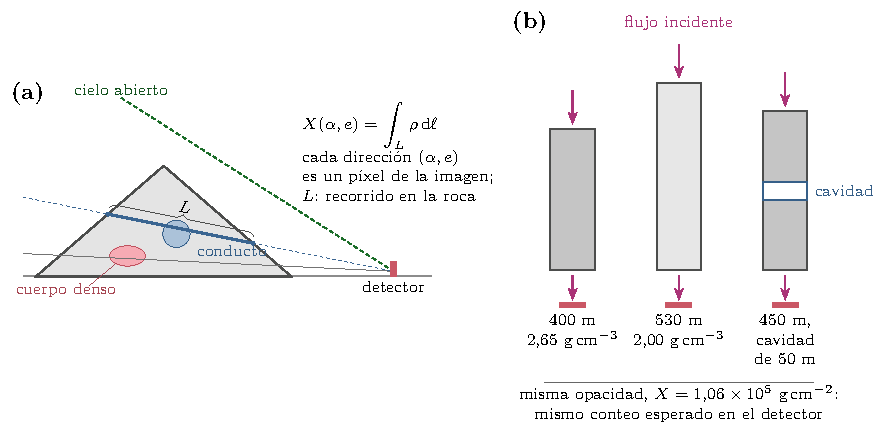
\includegraphics{fig2-1_opacidad_proyeccion.pdf}
\caption[La imagen muográfica por transmisión como proyección]{La imagen muográfica por transmisión como proyección (esquema sin escala). (a)~Cada dirección de observación $(\alpha,e)$ desde el detector define un trayecto; el píxel correspondiente registra la opacidad $X$ acumulada a lo largo del recorrido $L$ en la roca, incluidas las anomalías que encuentre, y la dirección de cielo abierto sirve de referencia para la transmisión. (b)~Ambigüedad entre espesor y densidad: 400~m de roca de 2,65~g\,cm$^{-3}$, 530~m de roca de 2,00~g\,cm$^{-3}$ y 450~m de roca de 2,65~g\,cm$^{-3}$ con una cavidad de 50~m tienen la misma opacidad, $1{,}06\times10^{5}$~g\,cm$^{-2}$, y producen el mismo conteo esperado. Fuente: elaboración propia.}
\label{fig:mt-proyeccion}
\end{figure}

Dos consecuencias se siguen de esa propiedad. La primera es que, para convertir la opacidad en una densidad, hace falta conocer la longitud del recorrido. La \cref{eq:mt-densidad-media} solo puede evaluarse si se conoce la superficie del terreno, normalmente mediante un modelo digital de elevación, y la posición del detector; sin esa información, la imagen no distingue entre una roca densa y una roca gruesa \parencite{lesparre2010,lechmann2021}. La segunda es que el problema inverso no tiene solución única. Como muestra el panel~(b) de la \cref{fig:mt-proyeccion}, distribuciones de densidad muy diferentes producen la misma opacidad y, por lo tanto, el mismo conteo esperado: una roca delgada y densa equivale a una gruesa y liviana, y una cavidad puede compensarse con un trayecto más largo. Por esta razón, la interpretación muográfica se apoya en contrastes. Se compara la opacidad o el conteo observado con el que produciría un modelo de referencia, por ejemplo el mismo edificio con densidad homogénea y topografía conocida, y se interpretan las desviaciones: un conducto de baja densidad produce un exceso de conteos respecto de su entorno y un cuerpo denso, un déficit.

Recuperar la distribución tridimensional de la densidad exige más información que la de una sola vista. Puede obtenerse combinando observaciones desde varias posiciones, en lo que constituye una tomografía muográfica, o mediante la inversión conjunta de los datos muográficos con otras mediciones, como las gravimétricas, que aportan sensibilidad a la masa en otras direcciones \parencite{nishiyama2022,lechmann2021,tanaka2023muography}. Con una sola vista, la muografía por transmisión entrega un mapa bidimensional de opacidad o de conteos, que es suficiente para localizar anomalías en el espacio de direcciones, pero no para situarlas en profundidad.

Las aplicaciones volcánicas de la técnica se han apoyado precisamente en esos mapas bidimensionales y en sus contrastes. Bajo el cráter del monte Asama se resolvió la estructura de densidad del fondo del cráter \parencite{tanaka2007asama}; en el Sakurajima, detectores gaseosos de trazas produjeron imágenes de alta definición y bajo ruido \parencite{olah2018sakurajima}, y en Colombia, el telescopio MuTe se diseñó para observar volcanes activos en zonas de difícil acceso, combinando paneles de centelleo con un detector Cherenkov de agua para filtrar el fondo \parencite{penarodriguez2020}. En todos los casos, la calidad de los contrastes obtenidos depende del número de muones registrados, que es el objeto de la sección siguiente.

% =============================================================================
\section{Estadística de conteo y tiempo de exposición}
\label{sec:mt-estadistica}

La llegada de muones a una celda angular del detector es una sucesión de eventos independientes y raros, que se modela como un proceso de Poisson. Si $\lambda$ es el número esperado de muones en la exposición $t$, de acuerdo con la \cref{eq:mt-conteo}, el conteo registrado $C$ sigue una distribución de Poisson, y de ella se derivan su valor esperado, su varianza y la relación entre la señal y el ruido:
\begin{subequations}\label{eq:mt-poisson}
\begin{align}
P(C=c) &= \frac{\lambda^{c}\,\mathrm{e}^{-\lambda}}{c!}, \qquad c=0,1,2,\dots, \label{eq:mt-poisson-pmf}\\
\mathrm{E}[C] &= \mathrm{Var}[C] = \lambda, \label{eq:mt-poisson-momentos}\\
\mathrm{SNR} &= \frac{\mathrm{E}[C]}{\sqrt{\mathrm{Var}[C]}} = \sqrt{\lambda}, \qquad \frac{\sqrt{\mathrm{Var}[C]}}{\mathrm{E}[C]} = \frac{1}{\sqrt{\lambda}}. \label{eq:mt-poisson-snr}
\end{align}
\end{subequations}
Todas las magnitudes de la \cref{eq:mt-poisson} son adimensionales. La señal, el número esperado de conteos, crece en proporción a la exposición; el ruido, medido por la desviación estándar, crece solo con su raíz cuadrada. En consecuencia, la relación señal-ruido es $\sqrt{\lambda}$ y el ruido relativo es $1/\sqrt{\lambda}$, como muestra la \cref{fig:mt-ruido}. Un píxel con un valor esperado de 100 conteos fluctúa típicamente un 10\,\%; uno con 10\,000 conteos, un 1\,\%. Para reducir el ruido relativo a la mitad hay que cuadruplicar la exposición, y reducir la exposición en un factor $k$ multiplica el ruido relativo por $\sqrt{k}$.

\begin{figure}[htbp]
\centering
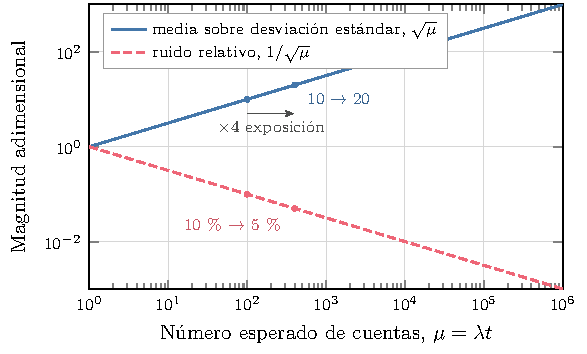
\includegraphics{fig2-2_ruido_conteo.pdf}
\caption[Relación señal-ruido y ruido relativo de un conteo de Poisson]{Relación señal-ruido, $\sqrt{\lambda}$, y ruido relativo, $1/\sqrt{\lambda}$, de un conteo de Poisson en función de su valor esperado $\lambda$, en escala logarítmica. Los puntos ilustran que cuadruplicar la exposición, de $\lambda=100$ a $\lambda=400$, duplica la relación señal-ruido y reduce el ruido relativo del 10 al 5\,\%. Curvas analíticas, sin datos del proyecto. Fuente: elaboración propia.}
\label{fig:mt-ruido}
\end{figure}

Esta dependencia determina el tiempo necesario para distinguir una anomalía. Si una anomalía cambia el número esperado de conteos de una región de $\lambda$ a $(1+\mathcal{C})\lambda$, donde $\mathcal{C}$ es el contraste relativo de la intensidad de conteo, el cambio solo se distingue de las fluctuaciones cuando supera algunas veces su desviación estándar. Si se exige que lo haga en $k$ desviaciones estándar, y se escribe $\lambda=r\,t$ con $r$ la tasa de conteo de la región, la condición y el tiempo de exposición que de ella resulta son
\begin{equation}\label{eq:mt-tiempo-deteccion}
|\mathcal{C}|\,\lambda \ge k\sqrt{\lambda}
\quad\Longleftrightarrow\quad
t \ge \frac{k^{2}}{\mathcal{C}^{2}\,r},
\end{equation}
donde $t$ y $1/r$ se expresan en la misma unidad de tiempo y $k$ y $\mathcal{C}$ son adimensionales. El tiempo necesario crece con el cuadrado del inverso del contraste: una anomalía con la mitad de contraste exige cuatro veces más exposición. Esta relación, de la misma naturaleza que el criterio de factibilidad formulado por \textcite{lesparre2010}, explica por qué las anomalías sutiles bajo grandes espesores de roca, donde la tasa $r$ es pequeña, exigen exposiciones de semanas o meses.

De lo anterior se sigue una precisión sobre el término \emph{alta estadística}. Una imagen de alta estadística no es una imagen sin azar, sino una con muchos conteos por píxel y, por lo tanto, con un ruido relativo pequeño, pero no nulo. Cuando una imagen de larga exposición se usa como referencia para juzgar otra, esa referencia conserva su propio ruido, y ninguna estimación puede coincidir exactamente con ella; la similitud alcanzable con una referencia finita tiene, por eso, un techo que depende de la estadística de la propia referencia.

El proceso de Poisson tiene, además, una propiedad que permite estudiar distintas exposiciones a partir de una sola medición o simulación. Si cada evento de un proceso de Poisson de media $\lambda$ se conserva de manera independiente con probabilidad $f$, los eventos conservados forman de nuevo un proceso de Poisson, de media $f\lambda$ \parencite{kingman1992}. En términos de conteos,
\begin{equation}\label{eq:mt-adelgazamiento}
C\sim\mathrm{Poisson}(\lambda), \quad C'\mid C\sim\mathrm{Bin}(C,f)
\quad\Longrightarrow\quad
C'\sim\mathrm{Poisson}(f\lambda), \qquad 0<f\le1,
\end{equation}
donde $C'$ es el conteo conservado y $f$ la fracción de conservación, ambos adimensionales. Como $f\lambda$ es el valor esperado que correspondería a una exposición $f\,t$, este adelgazamiento binomial produce, a partir de una imagen de exposición $t$, imágenes con la misma distribución que tendrían mediciones independientes de exposición $f\,t$. La equivalencia vale para cada imagen por separado: las imágenes reducidas que se obtienen de una misma imagen original comparten sus conteos y no son, entre sí, mediciones independientes.

% =============================================================================
\section{Aprendizaje profundo para la mejora de imágenes}
\label{sec:mt-aprendizaje}

La sección anterior mostró que el ruido de una imagen muográfica solo se reduce, por medios físicos, aumentando la exposición. La alternativa computacional consiste en estimar, a partir de la imagen ruidosa, la imagen que se habría obtenido con más exposición. Los filtros clásicos de suavizado reducen el ruido promediando píxeles vecinos, pero lo hacen a costa de la resolución espacial y difuminan precisamente los bordes y las anomalías pequeñas. El aprendizaje profundo aborda el problema de otro modo: aprende la relación entre imágenes degradadas y sus versiones de referencia a partir de ejemplos, y la aplica después a imágenes nuevas. Formalmente, dado un conjunto de pares formados por una entrada degradada $x$ y su referencia $y$, se ajustan los parámetros de una función $\hat y=G(x)$ para que su salida se aproxime a $y$ según una función de pérdida.

Las redes neuronales convolucionales son la arquitectura habitual para esta tarea. Cada capa aplica un conjunto de filtros que se aprenden durante el entrenamiento y que recorren la imagen con pesos compartidos, de modo que la red detecta un mismo patrón en cualquier posición y construye, capa tras capa, representaciones de escala creciente. La arquitectura U-Net, propuesta originalmente para la segmentación de imágenes biomédicas, organiza esas capas en un camino de contracción, que reduce la resolución y captura el contexto, y uno de expansión, que la recupera, unidos por conexiones de salto que transmiten directamente los detalles finos de cada escala \parencite{ronneberger2015}. Esa estructura la hace adecuada para transformar una imagen en otra del mismo tamaño, como se requiere al mejorar una imagen ruidosa.

La elección de la función de pérdida condiciona el tipo de estimación que se obtiene. Una pérdida que promedia el error cuadrático píxel a píxel conduce a la media condicional de las referencias compatibles con la entrada, y una que promedia el error absoluto, a su mediana. Ambas tienden a producir imágenes suaves, porque promedian las texturas posibles en lugar de elegir una de ellas \parencite{isola2017}. Las redes generativas antagónicas se propusieron, en parte, para superar esa limitación. En ellas, un generador $G$ produce muestras y un discriminador $D$ aprende a distinguirlas de los datos reales; ambos se entrenan como adversarios en el juego de la \cref{eq:mt-gan} \parencite{goodfellow2020}:
\begin{equation}\label{eq:mt-gan}
\min_{G}\max_{D}\;\mathrm{E}_{y\sim p_{\mathrm{datos}}}\!\left[\log D(y)\right]+\mathrm{E}_{z\sim p_{z}}\!\left[\log\!\left(1-D\!\left(G(z)\right)\right)\right],
\end{equation}
donde $p_{\mathrm{datos}}$ es la distribución de los datos reales, $z$ una variable aleatoria con distribución $p_{z}$ que alimenta al generador y $D(\cdot)\in(0,1)$ la probabilidad, estimada por el discriminador, de que su argumento provenga de los datos. En la versión condicional, generador y discriminador reciben además una información de entrada, de modo que el generador aprende una distribución condicionada por ella \parencite{mirza2014}. Para la traducción entre imágenes, \textcite{isola2017} combinaron un generador U-Net, condicionado por la imagen de entrada, con un discriminador que juzga parches locales de la imagen en lugar de la imagen completa, conocido como PatchGAN, y añadieron a la pérdida antagónica un término de error absoluto que mantiene la salida próxima a la referencia.

El entrenamiento de las redes generativas antagónicas es inestable cuando las distribuciones de los datos reales y de los generados apenas se solapan. \textcite{arjovsky2017} propusieron sustituir la divergencia implícita en la \cref{eq:mt-gan} por la distancia de Wasserstein, que sigue siendo informativa en ese caso y que, por la dualidad de Kantorovich y Rubinstein, se expresa como el máximo sobre las funciones 1-Lipschitz $h$. En esa formulación, el discriminador se convierte en un crítico que estima la distancia. \textcite{gulrajani2017} impusieron la restricción de Lipschitz mediante una penalización del gradiente del crítico en puntos interpolados entre datos reales y generados, lo que dio lugar a la variante WGAN-GP:
\begin{subequations}\label{eq:mt-wgan}
\begin{align}
W\!\left(P_{y},P_{\hat y}\right) &= \sup_{\|h\|_{L}\le1}\;\mathrm{E}_{y\sim P_{y}}\!\left[h(y)\right]-\mathrm{E}_{\hat y\sim P_{\hat y}}\!\left[h(\hat y)\right], \label{eq:mt-wgan-dual}\\
\mathcal{P}_{\mathrm{GP}} &= \lambda_{\mathrm{GP}}\;\mathrm{E}_{\tilde y}\!\left[\left(\left\|\nabla_{\tilde y}h(\tilde y)\right\|_{2}-1\right)^{2}\right], \qquad \tilde y=\alpha\,y+(1-\alpha)\,\hat y, \quad \alpha\sim\mathcal{U}(0,1), \label{eq:mt-wgan-gp}
\end{align}
\end{subequations}
donde $P_{y}$ y $P_{\hat y}$ son las distribuciones de las referencias y de las salidas del generador, $\|h\|_{L}$ la constante de Lipschitz del crítico $h$, $\tilde y$ un punto interpolado entre una referencia y una salida, y $\lambda_{\mathrm{GP}}$ el peso adimensional de la penalización. La combinación de la formulación condicional, la distancia de Wasserstein y la penalización de gradiente es la red generativa antagónica condicional de Wasserstein con penalización de gradiente, o cWGAN-GP.

Estas técnicas se han aplicado a un problema estrechamente análogo al de la muografía: la tomografía computarizada de baja dosis. Al reducir la dosis de radiación se reduce el número de fotones detectados y aumenta el ruido cuántico, de la misma naturaleza estadística que el de la \cref{eq:mt-poisson}. \textcite{yang2018} entrenaron una red generativa antagónica con distancia de Wasserstein y una pérdida perceptual para transformar tomografías de baja dosis en estimaciones de dosis normal, y mostraron que esa combinación preserva detalles y texturas que una pérdida de error cuadrático tiende a suavizar.

El uso de redes generativas para estimar imágenes tiene, sin embargo, dos límites que conviene tener presentes. El primero es un compromiso fundamental. \textcite{blau2018} demostraron que la distorsión de una estimación, medida por su distancia a la referencia, y su calidad perceptual, medida por la proximidad de su distribución a la de las imágenes reales, no pueden optimizarse a la vez más allá de cierto límite: una estimación con distorsión mínima tiende a ser suave y poco realista, y una con apariencia realista tiende a alejarse más de la referencia. Una red antagónica y una red entrenada solo con error absoluto ocupan, por lo tanto, puntos distintos de ese compromiso, y ninguna métrica aislada basta para compararlas. El segundo límite es el riesgo de alucinación. Las pérdidas que hacen coincidir la distribución de las salidas con la de las referencias pueden llevar al generador a añadir o eliminar estructuras de manera que la imagen resulte verosímil sin ser fiel a la entrada; \textcite{cohen2018} mostraron, en la traducción de imágenes médicas, que estas pérdidas pueden introducir o borrar lesiones cuando la distribución de entrenamiento no corresponde a la de los casos evaluados. En la muografía, donde una anomalía de densidad es precisamente la información buscada, este riesgo exige verificar que el modelo conserve las cuentas y los contrastes de las regiones de interés, y no solo la apariencia de la imagen.

% =============================================================================
\section{Aprendizaje automático en muografía}
\label{sec:mt-estado-arte}

El aprendizaje automático se ha incorporado a la muografía en varios puntos de la cadena de obtención de imágenes. La revisión de \textcite{luo2025} organiza las técnicas de reconstrucción en tres familias, la imagen por dispersión, la imagen por transmisión y la imagen con partículas secundarias, y para la transmisión examina las limitaciones del método clásico basado en la razón de flujos frente a algoritmos de inversión de densidad y de reconstrucción inversa inspirados en la imagenología médica. Sobre ese fondo, los trabajos que emplean aprendizaje automático pueden agruparse según la etapa en que intervienen.

En la etapa del detector, el aprendizaje automático se ha usado para separar los muones útiles del fondo. \textcite{galgoczi2024} entrenaron una red neuronal profunda, con muestras generadas por simulación Monte Carlo, para suprimir el fondo de baja energía en un sistema de detectores con capas absorbentes de plomo orientado a la muografía de volcanes, y obtuvieron una supresión considerablemente mejor que la del algoritmo clásico de trazas. El mismo problema del fondo motivó el diseño híbrido del telescopio colombiano MuTe, que lo aborda con instrumentación: un detector Cherenkov de agua y un sistema de tiempo de vuelo para descartar las partículas de las cascadas electromagnéticas y los eventos múltiples \parencite{penarodriguez2020}.

En la etapa de reconstrucción, la mayor parte de los trabajos se refiere a la tomografía por dispersión, que reconstruye volúmenes pequeños, como contenedores de carga, a partir de la desviación de cada muon. \textcite{sattler2025} desarrollaron un marco de reconstrucción diferenciable en PyTorch que integra métodos geométricos y un algoritmo de esperanza y maximización acelerado en GPU, evaluado con escenarios simulados en Geant4. \textcite{vinodkumar2025} combinaron la reconstrucción volumétrica por puntos de máxima aproximación con una red convolucional tridimensional que reduce el ruido de las reconstrucciones de materiales de número atómico alto, y \textcite{wang2026} entrenaron una U-Net con imágenes de tomografía por dispersión simuladas y la aplicaron a datos experimentales de exposición corta, con un aumento del índice de similitud estructural de 0,7232 a 0,9699.

En la etapa de mejora de la imagen, que es la de este trabajo, los antecedentes son más escasos. \textcite{lefevre2024} propusieron tres métodos de aprendizaje automático para la muografía con detectores Micromegas: un procedimiento de desmultiplexado de la lectura, una red neuronal para reducir el ruido estadístico de las imágenes, entrenada con muografías simuladas de varios cientos de reactores nucleares sintéticos, y una red de posprocesamiento tridimensional entrenada para compensar las limitaciones del algoritmo de tomografía; según los autores, estos métodos mejoraron de forma significativa las imágenes bidimensionales y las tomografías. \textcite{odonnell2025particles} aplicaron una cWGAN-GP a la mejora predictiva de imágenes muográficas de baja estadística de estructuras de concreto: según el índice de similitud estructural, imágenes de un día de exposición alcanzaron la calidad perceptual de imágenes de 21 días, y una segunda red, entrenada para segmentación, les permitió cuantificar el efecto de la mejora sobre los elementos internos de las muestras.

Esta revisión muestra que el aprendizaje profundo ya ha demostrado su capacidad para reducir el ruido estadístico de imágenes muográficas en varios escenarios, pero que, en los trabajos revisados, su aplicación a la muografía volcánica se ha concentrado en la supresión del fondo. En la literatura revisada no se identificó la aplicación de redes generativas condicionales a la mejora de imágenes de baja estadística de edificios volcánicos, un escenario cuyas distancias, espesores y contrastes difieren de los de las estructuras civiles o de los volúmenes de la tomografía por dispersión. Entrenar un modelo para ese escenario exige, como en los trabajos citados, datos simulados, cuyo papel y cuyos límites se examinan a continuación.

% =============================================================================
\section{Datos sintéticos y brecha entre simulación y realidad}
\label{sec:mt-simulacion}

El aprendizaje supervisado de la \cref{sec:mt-aprendizaje} requiere pares formados por una imagen de baja estadística y su referencia de alta estadística, y la muografía de campo no los proporciona. Una medición real no tiene una versión equivalente sin ruido, y repetirla con una exposición mucho mayor no garantiza que el objeto permanezca igual ni permite conocer su estructura interna verdadera. La simulación Monte Carlo resuelve esas dos carencias: produce imágenes de cualquier exposición sobre escenarios cuya estructura interna se conoce de antemano y, mediante el adelgazamiento binomial de la \cref{eq:mt-adelgazamiento}, permite derivar de una misma referencia entradas con distintas estadísticas de conteo.

La simulación del transporte de muones se basa en el muestreo aleatorio de los procesos físicos que una partícula sufre a lo largo de su trayectoria. Geant4 es un conjunto de herramientas de propósito general para esa tarea, que proporciona la descripción de la geometría y los materiales, los modelos de los procesos electromagnéticos y hadrónicos, el seguimiento paso a paso de las partículas y el registro de las magnitudes de interés, y cuya física ha sido validada de manera extensa por su comunidad de usuarios \parencite{agostinelli2003,allison2016}. Las partículas primarias se generan según el flujo de la \cref{sec:mt-muones}; EcoMug es un generador de muones cósmicos diseñado para hacerlo de manera eficiente a partir de parametrizaciones del flujo medido, con muones generados sobre superficies de distintas formas \parencite{pagano2021}. Como la mayoría de los muones generados no atraviesa la roca o no llega al detector, la eficiencia del muestreo condiciona en la práctica el costo computacional de una campaña de simulación muográfica.

La simulación tiene, sin embargo, un costo epistemológico: un modelo entrenado con datos simulados aprende la distribución de esos datos, y su desempeño sobre datos reales depende de cuánto se parezcan ambas distribuciones. En la muografía, la brecha entre simulación y realidad tiene varias fuentes. Los detectores reales tienen una eficiencia menor que la unidad, una aceptancia y una resolución angular finitas y un fondo de partículas que no son muones del objeto, cuyo peso relativo crece en las direcciones de mayor espesor, donde la señal es menor \parencite{lesparre2010,galgoczi2024,lechmann2021}. Los volcanes reales tienen una topografía irregular y una estructura de densidades heterogénea, con capas, fracturas, agua y variaciones graduales, que los escenarios simplificados no reproducen. Un modelo que no ha visto esas condiciones durante su entrenamiento puede degradarse al encontrarlas, de modo que el desempeño medido sobre datos simulados describe la capacidad del modelo dentro de la familia de escenarios simulados y no garantiza por sí solo su comportamiento en campo. La evaluación sobre escenarios simulados excluidos del entrenamiento mide la generalización dentro de esa familia; la transferencia a datos reales, como la que \textcite{wang2026} ensayaron en la tomografía por dispersión, requiere mediciones experimentales.

% =============================================================================
\section{Métricas de calidad de imagen}
\label{sec:mt-metricas}

Juzgar si una imagen mejorada se aproxima a su referencia exige métricas de referencia completa, que comparan dos imágenes píxel a píxel o región a región. La relación señal-ruido de pico, PSNR, transforma el error cuadrático medio entre la estimación y la referencia en una escala logarítmica, en decibelios, normalizada por el valor máximo posible de la imagen; mide la fidelidad punto a punto y es sensible a cualquier diferencia de amplitud. El índice de similitud estructural, SSIM, compara en ventanas locales la luminancia, el contraste y la estructura de ambas imágenes, con la motivación de aproximarse mejor a la percepción humana de la calidad \parencite{wang2004}. \textcite{hore2010} analizaron la relación matemática entre ambas medidas y mostraron que responden de manera diferente a distintos tipos de degradación, de modo que conviene informarlas juntas. Sus definiciones operativas en este trabajo se presentan en la sección~\ref{subsec:met-calidad}.

En la muografía, esas métricas no bastan. Están diseñadas para imágenes cuyo valor de píxel es una intensidad visual, mientras que en una imagen muográfica cada valor es un conteo con significado físico, ligado a la opacidad por la \cref{eq:mt-imagen}, y promedian sobre la imagen completa sin distinguir las regiones que importan para la interpretación. Una estimación puede, en consecuencia, aumentar su similitud global con la referencia y, al mismo tiempo, desplazar las cuentas de las regiones de roca o de las anomalías, lo que alteraría la opacidad que se infiere de ellas. Por esa razón, la evaluación de un modelo de mejora muográfica requiere, además, medidas físicamente motivadas: el sesgo de las cuentas integradas en regiones de interés, que indica si la estimación conserva la información de transmisión; el error en la franja del contorno del edificio, donde los gradientes de conteo son mayores y, como se vio en la \cref{sec:mt-interaccion}, la física ya difumina la transición, y el contraste de la intensidad de conteo de cada anomalía respecto de su entorno, que es la magnitud con la que se interpreta una imagen muográfica (\cref{sec:mt-imagen}). Junto con el compromiso entre distorsión y percepción y el riesgo de alucinación de la \cref{sec:mt-aprendizaje}, estas consideraciones justifican que la evaluación combine métricas de similitud con medidas de conservación de cuentas, de error de borde y de contraste, cuyas definiciones se presentan en la sección~\ref{subsec:met-anomalias}.

Con estos elementos quedan establecidos los fundamentos del trabajo: la física que liga la imagen con la densidad, la estadística que limita su calidad, los modelos capaces de estimar una imagen de mayor estadística, el antecedente que motiva su aplicación al escenario volcánico, el papel de los datos sintéticos y los criterios con los que debe juzgarse el resultado. El \cref{chap:metodologia} describe cómo se aplicaron.

\chapter{Metodología}
\label{chap:metodologia}

% Versión 4 del capítulo 3. Incorpora la metodología del OE2 y la parte sustentada del
% OE3 (repositorio muografia-documentada, rama principal en la revisión 08cdc0c).
% Versión 3: la parte del OE1 se actualizó a la campaña de 114 vistas.
% Sustento: repositorio muografia-documentada, rama principal en la revisión 4529c49
% y rama de entrega oe1/justificacion-fisica-produccion en la revisión 800ab86; los
% datos de la campaña corresponden a la entrega f395570.
% Los comentarios "% PENDIENTE" señalan asuntos para valorar con la dirección.

Este capítulo organiza la descripción del procedimiento experimental y computacional del proyecto: el diseño de la investigación, la generación de imágenes muográficas sintéticas, el desarrollo del modelo de aprendizaje profundo y el protocolo de evaluación. La estructura permite relacionar las decisiones y los procedimientos con los tres objetivos específicos aprobados. Los resultados cuantitativos, su interpretación y el balance de cumplimiento se desarrollan en el capítulo de Resultados y discusión.

% =============================================================================
\section{Diseño de la investigación y organización experimental}
\label{sec:met-diseno}

\subsection{Enfoque, alcance y unidad de análisis}
\label{subsec:met-enfoque}

La investigación se planteó como un estudio computacional. En lugar de adquirir datos en campo, el primer objetivo específico (OE1) se abordó mediante la simulación Monte Carlo del transporte de muones cósmicos a través de edificios volcánicos sintéticos, tal como lo establece su formulación aprobada: generar un conjunto de datos sintéticos de imágenes muográficas por transmisión, con diferentes niveles de estadística de conteo, que reproduzca escenarios representativos de exploración volcánica. La simulación ofrece dos ventajas que la adquisición real no permite: la estructura interna de cada escenario es conocida de antemano, y una misma referencia puede reducirse de forma controlada para obtener imágenes de distinta estadística a partir de un mismo experimento. El precio de esas ventajas es que ninguna conclusión de este capítulo se extiende, por sí sola, a mediciones de campo.

El procedimiento del OE1 abarcó la definición de los escenarios volcánicos, la configuración de la fuente de muones, el transporte de partículas y la formación de las imágenes, los ensayos de verificación previos a la producción, la campaña de simulación definitiva, la evaluación de la calidad de sus referencias, la reducción de la estadística de conteo, la partición del conjunto y los controles de integridad y de reproducción. La descripción que sigue se sustenta en el repositorio de referencia del proyecto, que conserva el código, las configuraciones, los registros de ejecución y las revisiones de la dirección de esa etapa\footnote{Repositorio \texttt{muografia-documentada}, \url{https://github.com/anlegogo/muografia-documentada}; rama principal en la revisión \texttt{4529c49} y rama de entrega de los estudiantes, \texttt{oe1/justificacion-fisica-produccion}, en la revisión \texttt{800ab86}. Los datos de la campaña corresponden a la entrega \texttt{f395570}.}. El entrenamiento de redes y la evaluación comparativa de modelos pertenecen a los objetivos segundo y tercero, y se describen en las secciones~\ref{sec:met-modelo} y~\ref{sec:met-evaluacion}.

Para delimitar correctamente las inferencias se distinguieron cuatro niveles de agregación. La \emph{geometría} es un escenario volcánico completo; el catálogo contiene diecinueve. La \emph{vista} es una posición del detector alrededor del edificio; cada geometría se observó desde seis vistas, para un total de 114. La \emph{realización} es una reducción aleatoria de los conteos de una vista a una fracción de ellos, obtenida por adelgazamiento binomial; por cada vista y fracción se generaron veinte realizaciones, de modo que cada vista aportó $4\times20=80$ pares de entrada y referencia, cada geometría 480 y el conjunto completo 9\,120. Finalmente, la \emph{ejecución de entrenamiento} corresponde al OE2 y no interviene en esta etapa.

Esta jerarquía determina la unidad de análisis. Las veinte realizaciones de una vista comparten la misma referencia y, por lo tanto, no constituyen escenarios volcánicos independientes; tampoco lo son los píxeles de una misma imagen. Por esa razón, la unidad de inferencia sobre escenarios es la geometría, y la partición del conjunto se hizo por geometrías completas (sección~\ref{subsec:met-particiones}). Aun así, separar geometrías no garantiza todas las formas de independencia experimental, de modo que las afirmaciones sobre escenarios no observados quedan restringidas al espacio que el catálogo representa.

Los objetivos segundo y tercero conservaron el carácter computacional. El modelo se entrenó y se evaluó exclusivamente con los pares sintéticos del OE1, de modo que su desempeño se refiere a referencias idealizadas de un catálogo conocido y no a mediciones de campo. A los tres niveles anteriores se añade, en esos objetivos, la ejecución de entrenamiento: una red obtenida con una configuración, un punto de partida y una semilla determinados. Las continuaciones de un mismo punto de control comparten su inicialización y no constituyen entrenamientos independientes, de modo que la variación entre ellas mide la estabilidad condicionada a ese punto de partida y no la variabilidad de entrenamientos desde cero. Como solo se dispuso de tres geometrías de prueba y de una de generalización, los resultados sobre geometrías no vistas se describen geometría por geometría y no se expresan como tasas poblacionales; tampoco permiten inferir el desempeño ante un volcán real ni ante las imágenes de un detector físico.

\subsection{Articulación de las etapas con los objetivos específicos}
\label{subsec:met-objetivos}

El OE1 se concibió como la etapa que produce el insumo de todo el proyecto: un conjunto de pares de imágenes de baja y alta estadística, con estructura interna conocida, sobre el cual se diseñan y evalúan los modelos de los objetivos siguientes. Sus entradas fueron el catálogo de escenarios volcánicos, las tablas de la fuente de muones, derivadas de una parametrización del flujo y del generador EcoMug, y una aplicación de transporte construida sobre Geant4 (secciones~\ref{subsec:met-geometrias}, \ref{subsec:met-fuente} y~\ref{subsec:met-transporte}). A partir de ellas se ejecutó una campaña de simulación por geometría y vista, se fusionaron sus bloques en una referencia por vista, se evaluó la calidad de las referencias, se redujo su estadística por adelgazamiento binomial y se particionó el conjunto, registrando en cada paso huellas de integridad que permiten comprobar que los productos no se alteraron (secciones~\ref{subsec:met-campana}, \ref{subsec:met-pares} y~\ref{subsec:met-particiones}). Los productos de la etapa son 114 histogramas de referencia con sus metadatos, las mismas referencias exportadas a un formato binario con coordenadas angulares explícitas, 114 archivos de pares, uno por vista, y los inventarios de huellas que los identifican.

La campaña definitiva fue precedida por una revisión técnica del conjunto inicial, que se había generado en agosto de 2026 con una configuración anterior de la cadena y se había congelado como versión~1.0. La revisión detectó defectos de construcción geométrica en seis escenarios y motivó una secuencia de ensayos acotados: la corrección de la geometría y la medición de su efecto sobre los conteos, la adopción de una nueva malla angular, el diagnóstico del observable registrado y de su normalización, y un piloto de seis vistas con la receta de producción (sección~\ref{subsec:met-verificacion}). Con esos resultados, la dirección del proyecto adoptó el 2 de octubre de 2026 un alcance idealizado para el producto del OE1, consistente en conteos direccionales sintéticos de transmisión con diferentes niveles de estadística, sin equivalencia con un instrumento real, y se fijaron de antemano el presupuesto y los criterios de calidad de la campaña. Las 114 referencias de esa campaña sustituyeron a las del conjunto inicial; ninguna referencia histórica se reutilizó.

El OE2 recibió como insumos los pares con fracción 0,05 de las particiones de entrenamiento y validación y la implementación de la red generativa condicional, revisada y corregida por la dirección antes de entrenar (sección~\ref{sec:met-modelo}). Su procedimiento comprendió un piloto, varios ajustes por continuación y un ensayo del error de borde, todos decididos con la partición de validación, y concluyó con la evaluación de ocho redes congeladas sobre las particiones reservadas, según un protocolo fijado antes de calcular sus métricas (sección~\ref{sec:met-evaluacion}). Sus productos son los pesos de las redes, identificados por sus huellas, sus predicciones y las métricas por imagen, por región y de contraste. Según el plan de trabajo, el OE3 consiste en evaluar el desempeño del modelo y determinar el factor de reducción del tiempo de adquisición, comparando las imágenes mejoradas con imágenes de exposición prolongada. Esa etapa reutilizó la evaluación final del OE2 y la complementó con un análisis descriptivo de la entrada sin red con cuatro fracciones de conteo (sección~\ref{subsec:met-factor}); la redacción oficial del objetivo y el criterio de calidad que exige la determinación del factor quedaron pendientes de confirmación por la dirección.

\subsection{Variables, factores y condiciones de comparación}
\label{subsec:met-variables}

El diseño del OE1 varió de forma controlada cuatro factores. El primero es el \emph{nivel de estadística}, definido como la fracción $f$ de los conteos de la referencia de una vista que se conserva en la imagen de entrada, con $f\in\{0{,}50;\ 0{,}10;\ 0{,}05;\ 0{,}01\}$. Cada referencia se obtuvo con un número fijo de $3{,}44\times10^{8}$ muones primarios por vista, de modo que una entrada con fracción $f$ representa, bajo los supuestos de la sección~\ref{subsec:met-pares}, una exposición $f$ veces menor del mismo observable. El segundo es el \emph{tipo de anomalía} de densidad, que puede ser un conducto, una cavidad o un cuerpo denso, presentes solos o combinados; una geometría de control, geo-train-01, carece de anomalías. El tercero es el \emph{contraste} de la anomalía, expresado como su diferencia de densidad respecto de la roca del edificio, de 2,65~g\,cm$^{-3}$. El cuarto combina la \emph{geometría}, que varía las dimensiones del edificio y la posición de las anomalías, con la \emph{vista}, que desplaza el detector en pasos de 60° alrededor del eje del cono.

Todas las demás condiciones se mantuvieron constantes en las 114 vistas: la receta de transporte, que fija la física, el tratamiento de las partículas secundarias, el punto de inyección y el umbral de registro; la malla angular; las tablas de la fuente, y el número de primarios (secciones~\ref{subsec:met-fuente} y~\ref{subsec:met-transporte}). La variable de respuesta es el número de muones primarios que alcanzan el plano de conteo con energía cinética superior a 3~GeV y cuya dirección de llegada cae en cada píxel angular. Para describir la calidad de las referencias se definieron, además, dos indicadores: la respuesta relativa en las regiones de borde de la ventana angular y la fracción de regiones de roca con al menos 100 cuentas (sección~\ref{subsec:met-verificacion}).

Se distinguió entre análisis confirmatorios, descriptivos y exploratorios. El criterio de bordes, el indicador de roca, sus regiones, el número de primarios y el tratamiento de las vistas que no alcanzaran la meta se registraron antes de enviar la campaña, y se prohibió modificarlos después de conocer los resultados; la evaluación de bordes tiene, por tanto, carácter confirmatorio, mientras que el indicador de roca se definió expresamente como descriptivo, sin valor de aceptación. En los ensayos previos, las regiones de interés, los efectos esperados y la partición de los resultados posibles también se fijaron antes de ejecutar las simulaciones. En cambio, la proporción global de regiones de roca con al menos 100 cuentas, agregada sobre todas las vistas, y las comparaciones con el motor analítico tienen carácter descriptivo o exploratorio. Esta distinción se mantiene al presentar los resultados en el capítulo~\ref{chap:resultados}.

En el OE2, el nivel de estadística se fijó en $f=0{,}05$ y el factor principal fue el método de recuperación: la entrada sin red, la U-Net entrenada con pérdida L1, la cGAN y las variantes de la cGAN ajustadas con los términos regional y de borde (\cref{tab:metodos-ef01}). Dentro de cada ensayo de ajuste se mantuvieron constantes el punto de partida, la semilla, el orden de las muestras y los hiperparámetros, y solo varió un término de la pérdida. Las variables de respuesta fueron el SSIM y el PSNR, que describen la semejanza global de la imagen, y el indicador regional de cuentas, los errores de cielo y de borde y el error de contraste de las anomalías, que describen la conservación física (secciones~\ref{subsec:met-calidad} y~\ref{subsec:met-anomalias}). Los ensayos de desarrollo se decidieron con reglas fijadas en sus diseños, sobre validación. La evaluación final siguió un protocolo fijado antes de abrir las particiones reservadas, pero, por la exposición previa de esas escenas, se clasificó como descriptiva y no como confirmatoria. La corrección numérica del contraste y las curvas de exposición del OE3 son análisis posteriores a la apertura de las reservas y tienen carácter descriptivo.

\subsection{Flujo general del procedimiento}
\label{subsec:met-flujo}

La generación del conjunto de datos se organizó como una cadena de etapas en la que cada una recibe los productos de la anterior junto con sus metadatos, de modo que cualquier imagen final puede rastrearse hasta el escenario, la receta, el bloque y la semilla que la produjeron. La \cref{fig:flujo} resume esa cadena. En su origen se encuentran dos insumos independientes: el catálogo de escenarios, generado de forma determinista a partir de una semilla, y las tablas de la fuente de muones. Los ensayos previos fijaron la receta de producción y el manifiesto de la campaña, que se congelaron con sus huellas antes del envío. La aplicación de transporte simuló cada vista en nueve bloques independientes, y cada bloque produjo un histograma angular acompañado de un recibo con su semilla, el número de primarios transportados y registrados y la huella de la receta empleada.

Los bloques se publicaron solo después de verificar su copia y su integridad, y los nueve de cada vista se fusionaron en una referencia. Las 114 referencias se evaluaron con los criterios fijados de antemano, se exportaron a un formato común con coordenadas angulares explícitas y se sometieron a adelgazamiento binomial para producir las entradas de baja estadística, agrupadas en un archivo de pares por vista. Por último, el conjunto se particionó por geometrías. En paralelo, una verificación independiente recalculó las huellas de archivo y de contenido de los productos. Las secciones siguientes describen cada etapa en el mismo orden.

\begin{figure}[htbp]
\centering
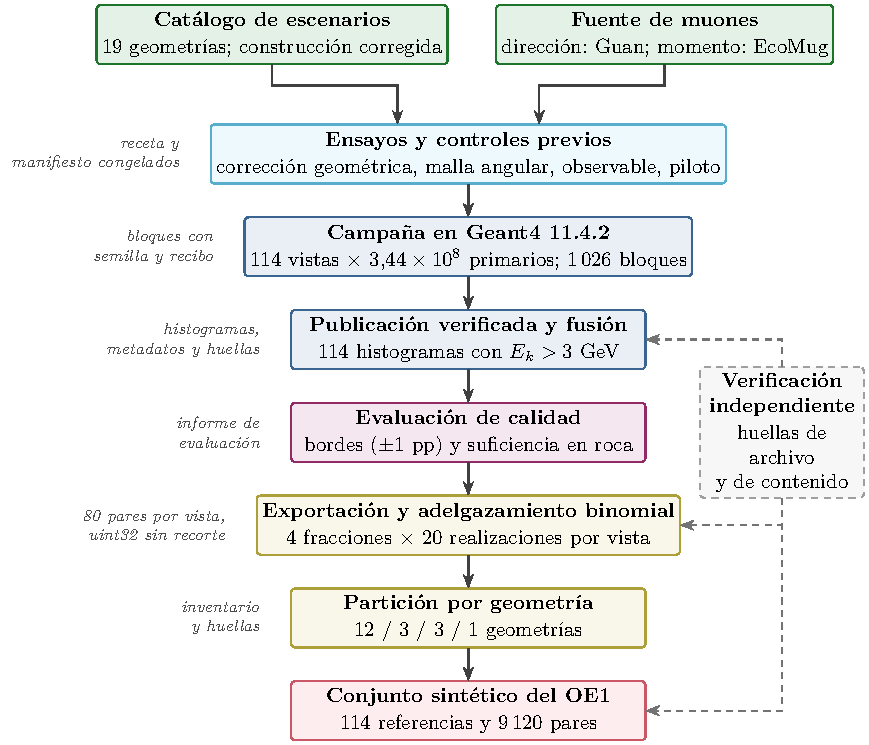
\includegraphics{fig3-1_flujo_oe1.pdf}
\caption[Cadena de generación y verificación del conjunto de datos (OE1)]{Cadena de generación y verificación del conjunto de datos sintéticos del OE1: insumos, ensayos y controles que fijaron la receta, campaña de Geant4 por bloques, publicación verificada y fusión, evaluación de calidad, exportación y adelgazamiento binomial, y partición por geometría. Las anotaciones de la izquierda indican los productos que enlazan cada etapa con la siguiente; la verificación independiente comprueba las huellas de archivo y de contenido. Fuente: elaboración propia a partir del repositorio de referencia.}
\label{fig:flujo}
\end{figure}

El desarrollo y la evaluación del modelo continuaron esa cadena a partir del conjunto particionado, como resume la \cref{fig:flujo-oe2}. Los pares de entrenamiento y validación, junto con la implementación corregida, alimentaron el piloto, cuyos pesos sirvieron de punto de partida a los ajustes por continuación y al ensayo de borde; durante todas esas etapas, el contrato de datos mantuvo cerradas las particiones de prueba y de generalización. Los pesos elegidos se congelaron por su huella en el contrato de la evaluación final, que se ejecutó después de registrar la procedencia de las particiones reservadas. Sus métricas se recalcularon de forma independiente, la selección de los controles de contraste recibió una corrección numérica y, por último, las mismas métricas se calcularon para la entrada sin red con cuatro fracciones de conteo. Cada etapa conservó, con sus productos, las configuraciones, los registros y las huellas que la enlazan con la anterior.

\begin{figure}[htbp]
\centering
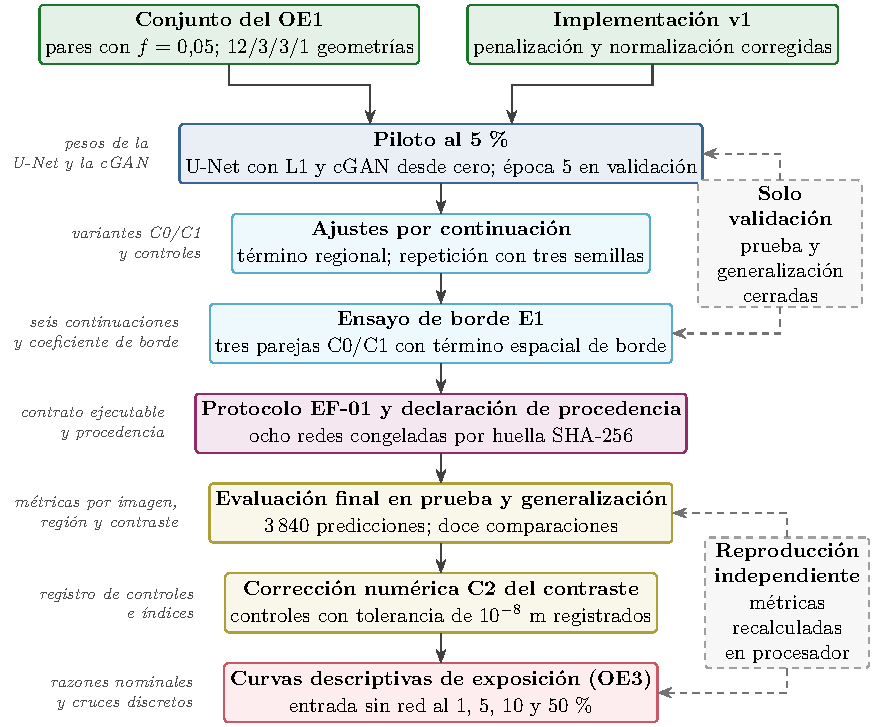
\includegraphics{fig3-6_flujo_oe2.pdf}
\caption[Desarrollo y evaluación del modelo (OE2) y análisis de exposición (OE3)]{Desarrollo y evaluación del modelo del OE2 y análisis descriptivo de exposición del OE3: insumos, ensayos decididos con validación, congelación de las redes y evaluación final, corrección numérica del contraste y curvas de exposición. Las anotaciones de la izquierda indican los productos que enlazan cada etapa con la siguiente; los recuadros discontinuos señalan la restricción de acceso a las particiones y la reproducción independiente de las métricas. Fuente: elaboración propia a partir del repositorio de referencia.}
\label{fig:flujo-oe2}
\end{figure}

% =============================================================================
\section{Generación y preparación del conjunto de datos sintéticos}
\label{sec:met-datos}

\subsection{Definición de los escenarios volcánicos y las anomalías}
\label{subsec:met-geometrias}

Cada escenario representó el edificio volcánico como un cono recto de radio basal $R$ y altura $H$, compuesto por roca homogénea de densidad 2,65~g\,cm$^{-3}$, en cuyo interior se insertaron anomalías de tres tipos: conductos de menor densidad, cavidades casi vacías y cuerpos más densos que la roca. Esta representación idealiza tres estructuras de interés en la exploración volcánica y mantiene, al mismo tiempo, espesores de roca de cientos de metros a algo más de un kilómetro a lo largo de las líneas de visión, el intervalo en el que la muografía por transmisión es factible con detectores de pocos metros cuadrados \parencite{lesparre2010,lechmann2021}. Las simplificaciones son deliberadas y explícitas: simetría cónica, roca de densidad única, anomalías de forma geométrica elemental con densidad uniforme y ausencia de topografía circundante. El alcance de la representatividad que se deriva de ellas se discute al final de esta sección.

El catálogo se generó de forma determinista. Cada geometría recibió una receta que fija su partición y su combinación de anomalías, y sus parámetros se muestrearon de distribuciones uniformes con un generador pseudoaleatorio independiente por geometría, derivado de una semilla común de valor 20260805 \parencite{harris2020}; así, el catálogo completo puede regenerarse exactamente. El diseño exigió que cada tipo de anomalía apareciera solo y en combinación con los demás, e incluyó una geometría de control sin anomalías y una geometría de generalización reservada fuera de toda partición de ajuste. La \cref{tab:rangos} presenta la parametrización del muestreo: el conducto es un cilindro vertical que parte de la base del edificio, la cavidad es una esfera y el cuerpo denso es un elipsoide de semiejes alineados con los ejes coordenados. En cavidades y cuerpos densos, el centro se desplazó del eje una fracción aleatoria del margen disponible, $\max\!\big(R(1-z_c/H)-r_h-20;\;30\big)$~m, donde $z_c$ es la altura del centro y $r_h$ el radio de la cavidad o el mayor semieje horizontal del cuerpo denso; el ángulo azimutal del centro fue uniforme en $[0;\,2\pi)$. Las longitudes se redondearon a 0,1~m y las densidades a tres decimales.

\begin{table}[htbp]
\centering
\caption[Parametrización del muestreo de los escenarios volcánicos]{Parametrización del muestreo de los escenarios volcánicos. $\mathcal{U}(a;\,b)$ denota una distribución uniforme en $[a;\,b]$; $H$ es la altura del edificio, $R$ su radio basal, $z_0$ y $z_1$ las alturas inferior y superior del conducto, $c_x$ y $c_y$ las coordenadas horizontales de su eje y $z_c$ la altura del centro de la anomalía. Fuente: elaboración propia a partir del generador del catálogo del repositorio de referencia.}
\label{tab:rangos}
\small
\begin{tabularx}{\linewidth}{@{}lX@{}}
\toprule
Elemento & Parámetros \\
\midrule
Edificio (cono) & $R\sim\mathcal{U}(500;\,700)$~m; $H\sim\mathcal{U}(350;\,450)$~m; densidad de la roca 2,65~g\,cm$^{-3}$ (fija) \\
Conducto (cilindro) & radio $\mathcal{U}(15;\,40)$~m; densidad $\mathcal{U}(1{,}8;\,2{,}2)$~g\,cm$^{-3}$; $c_x,c_y\sim\mathcal{U}(-40;\,40)$~m; $z_0=0$; $z_1=\mathcal{U}(0{,}75;\,0{,}95)\,H$ \\
Cavidad (esfera) & radio $\mathcal{U}(20;\,50)$~m; densidad $\mathcal{U}(0{,}0;\,0{,}5)$~g\,cm$^{-3}$; $z_c=\mathcal{U}(0{,}25;\,0{,}55)\,H$; desplazamiento radial $\mathcal{U}(0{,}1;\,0{,}6)$ del margen disponible \\
Cuerpo denso (elipsoide) & semiejes $a_x,a_y\sim\mathcal{U}(40;\,90)$~m, $a_z\sim\mathcal{U}(30;\,70)$~m; densidad $\mathcal{U}(3{,}0;\,3{,}3)$~g\,cm$^{-3}$; $z_c=\mathcal{U}(0{,}15;\,0{,}45)\,H$; desplazamiento radial $\mathcal{U}(0{,}1;\,0{,}5)$ del margen disponible \\
\bottomrule
\end{tabularx}
\end{table}

El resultado de ese muestreo es el catálogo de diecinueve escenarios que recoge la \cref{tab:catalogo}: doce destinados al entrenamiento, tres a la validación, tres a la prueba y uno a la evaluación de generalización. La tabla enumera, para cada geometría, las dimensiones del edificio y la densidad y el tamaño de cada anomalía en el orden en que se declararon, orden que resulta relevante cuando dos anomalías se superponen.

\begin{table}[htbp]
\centering
\caption[Catálogo de escenarios volcánicos sintéticos]{Catálogo de escenarios volcánicos sintéticos. C: conducto (densidad en g\,cm$^{-3}$; radio $r$ en m); V: cavidad (densidad; radio); D: cuerpo denso (densidad; semiejes $a_x/a_y/a_z$ en m). La densidad de la roca es 2,65~g\,cm$^{-3}$ en todos los casos; las anomalías se listan en el orden de declaración. Fuente: elaboración propia a partir del catálogo del repositorio de referencia.}
\label{tab:catalogo}
\footnotesize
\begin{tabularx}{\linewidth}{@{}llrrX@{}}
\toprule
Geometría & Partición & $R$ (m) & $H$ (m) & Anomalías \\
\midrule
geo-train-01 & entrenamiento & $656{,}2$ & $359{,}1$ & ninguna (control) \\
geo-train-02 & entrenamiento & $549{,}7$ & $409{,}8$ & C ($1{,}920$; $r=19{,}9$) \\
geo-train-03 & entrenamiento & $573{,}7$ & $356{,}2$ & V ($0{,}267$; $r=35{,}8$) \\
geo-train-04 & entrenamiento & $679{,}8$ & $387{,}2$ & D ($3{,}022$; $78{,}1/62{,}8/40{,}7$) \\
geo-train-05 & entrenamiento & $565{,}7$ & $386{,}0$ & C ($2{,}013$; $r=28{,}2$); V ($0{,}335$; $r=29{,}4$) \\
geo-train-06 & entrenamiento & $509{,}7$ & $416{,}3$ & C ($1{,}832$; $r=21{,}0$); D ($3{,}285$; $72{,}9/61{,}6/64{,}6$) \\
geo-train-07 & entrenamiento & $678{,}7$ & $429{,}2$ & V ($0{,}169$; $r=48{,}0$); D ($3{,}015$; $70{,}3/65{,}8/46{,}4$) \\
geo-train-08 & entrenamiento & $588{,}2$ & $413{,}4$ & C ($1{,}991$; $r=35{,}4$); V ($0{,}468$; $r=20{,}2$); D ($3{,}256$; $43{,}2/62{,}2/57{,}2$) \\
geo-train-09 & entrenamiento & $549{,}4$ & $373{,}2$ & C ($1{,}884$; $r=18{,}4$) \\
geo-train-10 & entrenamiento & $648{,}7$ & $449{,}6$ & V ($0{,}464$; $r=27{,}9$); V ($0{,}068$; $r=45{,}7$) \\
geo-train-11 & entrenamiento & $623{,}0$ & $419{,}8$ & C ($1{,}972$; $r=22{,}7$); V ($0{,}327$; $r=42{,}5$); V ($0{,}157$; $r=48{,}9$) \\
geo-train-12 & entrenamiento & $534{,}5$ & $411{,}9$ & D ($3{,}159$; $57{,}5/57{,}4/39{,}5$) \\
geo-val-01 & validación & $698{,}7$ & $427{,}6$ & C ($2{,}071$; $r=25{,}3$) \\
geo-val-02 & validación & $664{,}0$ & $367{,}3$ & V ($0{,}208$; $r=38{,}8$) \\
geo-val-03 & validación & $610{,}9$ & $425{,}4$ & C ($1{,}850$; $r=22{,}5$); D ($3{,}014$; $65{,}5/68{,}5/34{,}5$) \\
geo-test-01 & prueba & $671{,}1$ & $428{,}0$ & C ($2{,}151$; $r=30{,}3$); V ($0{,}454$; $r=36{,}5$) \\
geo-test-02 & prueba & $642{,}2$ & $415{,}9$ & D ($3{,}090$; $52{,}3/41{,}9/39{,}6$) \\
geo-test-03 & prueba & $518{,}5$ & $385{,}8$ & C ($1{,}914$; $r=30{,}2$); V ($0{,}222$; $r=24{,}1$); D ($3{,}244$; $74{,}2/55{,}3/64{,}9$) \\
geo-gen-01 & generalización & $619{,}2$ & $425{,}4$ & C ($1{,}831$; $r=26{,}1$); V ($0{,}242$; $r=40{,}9$); V ($0{,}048$; $r=42{,}4$) \\
\bottomrule
\end{tabularx}
\end{table}

La \cref{fig:catalogo} muestra un corte vertical de densidad de cada escenario, trazado por el plano que atraviesa la primera anomalía. Los cortes se calcularon con el campo de materiales del motor analítico que se describe en la sección~\ref{subsec:met-campana}, no con la construcción de Geant4, y permiten apreciar la variedad de tamaños, profundidades y combinaciones del catálogo.

\begin{figure}[htbp]
\centering
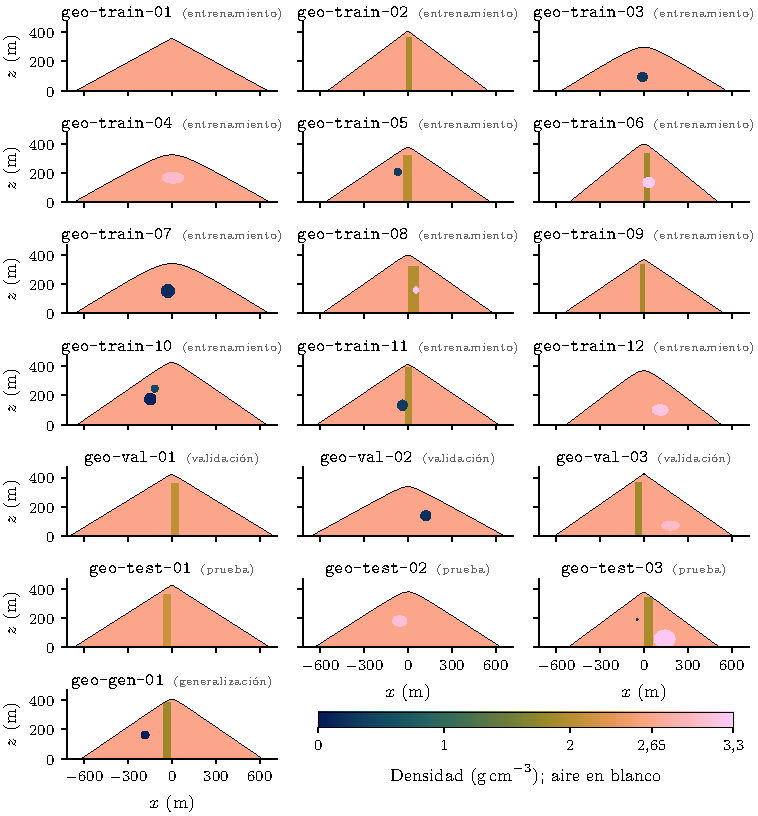
\includegraphics{fig3-2_catalogo_cortes.pdf}
\caption[Cortes verticales de densidad de los diecinueve escenarios]{Cortes verticales $x$--$z$ de densidad de los diecinueve escenarios del catálogo, por el plano $y$ que atraviesa la primera anomalía de cada geometría, calculados con el campo de materiales del motor analítico, a la misma escala horizontal y vertical. El aire se muestra en blanco. Fuente: elaboración propia a partir del catálogo del repositorio de referencia.}
\label{fig:catalogo}
\end{figure}

En la aplicación de transporte, basada en Geant4 \parencite{agostinelli2003,allison2016}, el edificio se construyó como un cono truncado con radio de vértice de 0,1~m, apoyado sobre el plano $z=0$ dentro de un volumen de aire. La roca se modeló como SiO$_2$ con la densidad del escenario, y cualquier densidad inferior a 0,05~g\,cm$^{-3}$ se sustituyó por aire, regla que en el catálogo afecta únicamente a la segunda cavidad de geo-gen-01. Cada anomalía se representó con su sólido elemental, del mismo material con su densidad propia, y se colocó como volumen hijo del edificio. En el conjunto inicial, las anomalías se colocaron completas, sin recortarlas al edificio ni restarlas entre sí, mientras que el motor analítico recorta cada anomalía al edificio y asigna a una región compartida la densidad de la última anomalía declarada; por esa diferencia, un mismo escenario no producía necesariamente el mismo campo de materiales en ambos motores cuando dos anomalías se superponían o una de ellas sobresalía del edificio. En la campaña definitiva, todas las geometrías se construyeron con la regla de corrección que se describe en la sección~\ref{subsec:met-verificacion}, la cual reproduce la convención del motor analítico.

La contención y el solapamiento de volúmenes se controlaron en dos niveles. Durante la construcción, Geant4 verificó cada colocación y emitió advertencias de superposición en el registro de la ejecución, sin detenerla. Sobre el catálogo se aplicó, además, una auditoría analítica independiente de la simulación. Para cada par de anomalías, la auditoría descartó la intersección solo mediante pruebas suficientes, como cajas envolventes disjuntas o distancias exactas entre esferas y cilindros; en los demás casos buscó puntos estrictamente interiores a ambos sólidos en una malla de $33\times33\times33$ puntos sobre la región común de sus cajas envolventes, y declaró el par intersectado solo al encontrar un testigo interior, dejando como no resuelta una búsqueda sin testigo. La contención de un conducto en el edificio se evaluó comparando su máximo radio ocupado, $\sqrt{c_x^2+c_y^2}+r$, con el radio del cono a la altura de su extremo superior, dado por la \cref{eq:radio-cono},
\begin{equation}
R(z)=R-(R-0{,}1)\,\frac{z}{H},
\label{eq:radio-cono}
\end{equation}
donde $R(z)$ es el radio del cono construido en Geant4 a la altura $z$, en metros, y 0,1~m su radio de vértice; para esferas y elipsoides se emplearon cotas suficientes y sus extremos verticales. Ninguno de los dos controles reproduce la navegación de las partículas, de modo que la ausencia de defectos en ellos no certifica por sí sola la geometría efectivamente transportada. Las superposiciones detectadas en el conjunto inicial motivaron la corrección y los ensayos descritos en la sección~\ref{subsec:met-verificacion}.

\paragraph{Representatividad dentro del alcance adoptado.}
% PENDIENTE (valoración de la dirección, criterio A-02): este apartado integra el
% borrador de representatividad de la rama de entrega (REPRESENTATIVIDAD_A02.md).
Bajo el alcance idealizado que adoptó la dirección, la representatividad del conjunto se entendió como la cobertura de una familia de edificios cónicos con heterogeneidades internas del tipo que la muografía volcánica asocia con conductos, cavidades y cuerpos densos \parencite{tanaka2007asama,olah2018sakurajima,tanaka2023muography}, observados en geometría de transmisión. No se pretendió que las geometrías reprodujeran un volcán concreto ni que las imágenes equivalieran a las de un instrumento real. Dentro de esa familia, el catálogo cubre edificios de 509,7 a 698,7~m de radio basal y de 356,2 a 449,6~m de altura; once conductos, en once geometrías, con densidades de 1,831 a 2,151~g\,cm$^{-3}$ y radios de 18,4 a 35,4~m; trece cavidades, en diez geometrías, con densidades de 0,048 a 0,468~g\,cm$^{-3}$ y radios de 20,2 a 48,9~m, y ocho cuerpos densos, en ocho geometrías, con densidades de 3,014 a 3,285~g\,cm$^{-3}$ y semiejes de 34,5 a 78,1~m. Las anomalías presentan contrastes de ambos signos respecto de la roca y aparecen solas y combinadas, incluidas dos geometrías con los tres tipos. La geometría de generalización repite la combinación de geo-train-11, con otros tamaños y posiciones, de modo que evalúa la generalización a nuevas configuraciones de anomalías conocidas y no a un tipo nuevo de anomalía.

En el cono homogéneo de cada geometría, el percentil 90 del espesor másico nominal de los rayos que cruzan roca va de $2{,}13\times10^{5}$ a $2{,}96\times10^{5}$~g\,cm$^{-2}$, y entre el 70,7 y el 87,1\,\% de las celdas de $4\times4$ píxeles con roca superan $10^{5}$~g\,cm$^{-2}$; las imágenes abarcan, por tanto, desde el cielo abierto hasta opacidades altas. El plan de trabajo preveía perfiles inspirados en topografías reales, como las de los volcanes Asama o Sakurajima, adaptados a geometrías simplificadas; el catálogo empleó conos, y esa simplificación se declara como una limitación del conjunto. La fuente y el transporte, descritos en las dos subsecciones siguientes, son únicos y trazables para las 114 vistas, y la tarea de los objetivos posteriores depende de la relación entre conteos de distinta estadística bajo esa definición común, no de una escala absoluta de flujo. Esa justificación respalda la representatividad dentro de la familia idealizada; no respalda la reproducción de un volcán concreto, un flujo calibrado ni la equivalencia con un detector. La valoración académica de este criterio corresponde a la dirección del proyecto.

\subsection{Configuración de la fuente de muones}
\label{subsec:met-fuente}

La fuente de muones debía cumplir dos requisitos: reproducir la distribución direccional del flujo con la misma convención que el motor analítico, para que ambas simulaciones fueran comparables, y conservar la física de un generador de muones cósmicos establecido. Para satisfacerlos se combinaron dos modelos. La dependencia direccional y la normalización se tomaron de la parametrización del flujo a nivel del mar de \textcite{guan2015muonflux}, que modifica la fórmula de Gaisser \parencite{gaisser2016} para energías bajas y ángulos cenitales grandes. El espectro de momento y la razón de carga se tomaron del generador EcoMug \parencite{pagano2021}.

EcoMug se empleó en una generación directa, independiente de Geant4, que produjo una muestra de $10^7$ muones desde un plano horizontal de cielo, con momento entre 0,5 y 10\,000~GeV/$c$ y semilla 20260805. A partir de esa muestra y de la parametrización de Guan se construyeron tres tablas que la aplicación de transporte consulta durante la simulación, sin invocar EcoMug en tiempo de ejecución. La primera asigna a cada una de las 256 filas angulares de elevación un peso proporcional al número esperado de muones de cielo abierto; la segunda almacena, para 16 bandas de elevación entre 2° y 47°, los cuantiles de la distribución del momento; y la tercera registra la razón de carga medida en la muestra. En la campaña definitiva, la generación se extendió 5° fuera de la ventana de observación, con el fin de compensar la migración angular de los muones desde el exterior de la ventana: el acimut se generó de manera uniforme en $\pm35^{\circ}$, los pesos de las ocho filas más próximas a cada borde de elevación se extrapolaron linealmente fuera del intervalo tabulado, con los pesos negativos anulados, y fuera del intervalo de las bandas de momento se empleó la banda extrema más cercana. La \cref{tab:generador} resume esa configuración.

\begin{table}[htbp]
\centering
\caption[Configuración de la fuente de muones]{Configuración de la fuente de muones de la campaña definitiva: muestra de EcoMug, tablas derivadas y extensión de la generación. Fuente: elaboración propia a partir de la receta operativa y de las tablas del generador del repositorio de referencia.}
\label{tab:generador}
\small
\begin{tabularx}{\linewidth}{@{}>{\raggedright\arraybackslash}p{5.0cm}>{\raggedright\arraybackslash}X@{}}
\toprule
Elemento & Valor registrado \\
\midrule
Versión de EcoMug & 2.2 (cabecera incluida en el código) \\
Muestra de EcoMug & $10^7$ muones; momento 0,5--10\,000~GeV/$c$; semilla 20260805 \\
Pesos por fila de elevación & 256 filas entre 2° y 47°, proporcionales al conteo de cielo abierto; ocho filas de borde extrapoladas linealmente fuera del intervalo \\
Distribución del momento & 16 bandas de elevación entre 2° y 47°; 257 cuantiles por banda; interpolación lineal; banda extrema fuera del intervalo \\
Razón de carga $\rho_{\pm}=\mu^+/\mu^-$ & 1,2794 \\
Ventana de generación & acimut relativo $\pm35^{\circ}$ (margen de 5° sobre la ventana de conteo) \\
Probabilidad de dirección nominal en la ventana, $p_{\mathrm{nom}}$ & 0,6841465610 \\
Escala convencional, $S_0$ & $36\,034\,069{,}91$ muones por 30 días convencionales \\
\bottomrule
\end{tabularx}
\end{table}

Las magnitudes que definen el muestreo y su normalización se agrupan en la \cref{eq:fuente}. El conteo esperado de cielo abierto en el píxel $(i,j)$, de la fila de elevación $i$ y la columna de acimut $j$, sigue la convención de aceptancia del protocolo de simulación (\cref{eq:fuente-lambda}); su suma sobre las columnas da el peso de cada fila, $\lambda_i$, y la suma de los pesos de todas las filas da la escala $S_0$ (\cref{eq:fuente-s0}). La fila de una dirección se elige con la probabilidad $w_i$ de la \cref{eq:fuente-w}, la carga positiva con la probabilidad de la \cref{eq:fuente-carga}, y la exposición convencional de una vista se obtiene de su número de direcciones nominales en la ventana según la \cref{eq:fuente-t}:
\begin{subequations}\label{eq:fuente}
\begin{align}
\lambda_{\mathrm{open},ij} &= \Phi_{\mathrm{int}}\,A\,\Delta\Omega_{ij}\,t, \qquad \lambda_i=\sum_{j=1}^{256}\lambda_{\mathrm{open},ij}, \label{eq:fuente-lambda}\\
S_0 &= \sum_{i=1}^{256}\lambda_i, \label{eq:fuente-s0}\\
w_i &= \frac{\lambda_i}{S_0}, \label{eq:fuente-w}\\
P(\mu^+) &= \frac{\rho_{\pm}}{1+\rho_{\pm}}, \label{eq:fuente-carga}\\
T_v &= 30\,\frac{N_{\mathrm{nom},v}}{S_0}. \label{eq:fuente-t}
\end{align}
\end{subequations}
En estas expresiones, $\Phi_{\mathrm{int}}$ es el flujo integral de muones de cielo abierto en la dirección del píxel, por encima de la energía mínima de 0,798~GeV, que en la convención heredada corresponde al frenado continuo en 367,5~g\,cm$^{-2}$ de aire, en cm$^{-2}$\,s$^{-1}$\,sr$^{-1}$; $A=1{,}44\times10^{4}$~cm$^{2}$ es el área de detección, tomada normal a cada dirección; $\Delta\Omega_{ij}=\Delta\alpha\,\Delta e\,\cos e_i$ es el ángulo sólido del píxel, en sr; $t$ es la duración de 30 días expresada en segundos; $\rho_{\pm}$ es la razón de carga de la \cref{tab:generador}; $N_{\mathrm{nom},v}$ es el número de primarios de la vista $v$ cuya dirección nominal cae dentro de la ventana de conteo, que se registró exactamente en cada bloque, y $T_v$ es la exposición convencional de la vista, en días convencionales. A diferencia del conjunto inicial, en el que el número de eventos de una simulación se sorteaba según una distribución de Poisson de media proporcional a la exposición, en la campaña definitiva cada vista recibió un número fijo de primarios, $N_v=3{,}44\times10^{8}$, de los cuales aproximadamente la fracción $p_{\mathrm{nom}}$ tiene dirección nominal en la ventana. La exposición $T_v$ es, por tanto, una etiqueta derivada de los supuestos del modelo de flujo y del área de detección, y no la duración de una medición de un detector real.

El algoritmo~\ref{alg:primario} describe cómo se generó cada muon a partir de esas tablas. La elevación se obtiene de la fila elegida más una perturbación uniforme de medio paso, el acimut es uniforme en la ventana de generación y el momento se obtiene invirtiendo la distribución acumulada de la banda correspondiente. La energía cinética se calcula como $E_k=\sqrt{p^2+m_\mu^2}-m_\mu$, en GeV, con $m_\mu=0{,}1056583745$~GeV/$c^2$ y $c=1$. El punto de inyección se sitúa sobre la trayectoria nominal que termina en el panel detector, según se explica en la sección~\ref{subsec:met-transporte}. Esta combinación reproduce la aceptancia direccional del motor analítico, de modo que las diferencias entre ambos motores reflejan la física del transporte, mientras que el espectro conserva la física del generador. El espectro de EcoMug es más blando que el de Guan, con distancias de Kolmogórov--Smirnov entre 0,063 y 0,119 según la banda de elevación; esa diferencia, junto con la masa de probabilidad que procede de las filas extrapoladas, forma parte de las hipótesis comunes del conjunto y no de un flujo calibrado.

\begin{algorithm}[htbp]
\caption{Generación dirigida de un muon primario a partir de las tablas del generador}
\label{alg:primario}
\begin{algorithmic}[1]
\Require pesos de fila $\{w_i\}$, incluidas las filas extrapoladas; cuantiles de momento por banda de elevación; razón de carga $\rho_{\pm}$; posición y orientación del panel detector; geometría del edificio; generador pseudoaleatorio inicializado con la semilla del bloque
\Ensure dirección, momento, carga y punto de inyección de un muon primario
\State elegir la fila de elevación $i$ con probabilidad $w_i$ mediante la distribución acumulada de los pesos
\State $e \gets$ centro de la fila $i$ más una perturbación uniforme en $\pm$ medio paso de fila
\State $\alpha \gets$ acimut relativo uniforme en $[-35^{\circ};\,35^{\circ}]$
\State $p \gets$ inversión de la distribución acumulada del momento en la banda de $e$, con interpolación lineal entre cuantiles
\State asignar carga positiva con probabilidad $\rho_{\pm}/(1+\rho_{\pm})$ y carga negativa en otro caso
\State $E_k \gets \sqrt{p^2+m_\mu^2}-m_\mu$
\State $\mathbf{x}_{\mathrm{imp}} \gets$ punto uniforme sobre la superficie del panel detector
\State muestrear la recta que parte de $\mathbf{x}_{\mathrm{imp}}$ hacia el cielo en la dirección $(e,\alpha)$ cada 0,5~m, hasta 4~km
\If{algún punto muestreado cae dentro del cono}
  \State $\mathbf{x}_0 \gets$ último punto interior encontrado, desplazado 1~m hacia el cielo
\Else
  \State $\mathbf{x}_0 \gets$ punto situado 1~m antes del panel sobre la misma recta
\EndIf
\State \Return $(\mathbf{x}_0,\ e,\ \alpha,\ E_k,\ \text{carga})$
\end{algorithmic}
\end{algorithm}

\subsection{Transporte de partículas y representación del detector en Geant4}
\label{subsec:met-transporte}

El transporte se simuló con una aplicación desarrollada sobre Geant4 11.4.2, con la lista de física \texttt{FTFP\_BERT}. Como la variable de interés es el número de muones primarios que atraviesan el edificio, toda partícula secundaria se eliminó en el momento de su creación y solo se transportó el muon primario. Esta decisión reduce el costo computacional sin alterar la transmisión de primarios, aunque excluye del modelo los fondos producidos por secundarios. La ejecución se hizo en modo multihilo, con 64 hilos por bloque, y la semilla de cada bloque inicializó el generador de Geant4. La \cref{tab:geant4} resume la configuración del transporte y del registro.

\begin{table}[htbp]
\centering
\caption[Configuración del transporte y del registro en Geant4]{Configuración del transporte y del registro en Geant4 en la campaña definitiva. Fuente: elaboración propia a partir de la receta operativa y de los metadatos de la campaña del repositorio de referencia.}
\label{tab:geant4}
\small
\begin{tabularx}{\linewidth}{@{}lX@{}}
\toprule
Elemento & Configuración \\
\midrule
Geant4 & versión 11.4.2, modo multihilo; 64 hilos por bloque \\
Física & \texttt{FTFP\_BERT}; solo primarios, secundarios eliminados al crearse \\
Edificio y anomalías & cono de radio de vértice 0,1~m; roca SiO$_2$ a la densidad del escenario; anomalías construidas con la regla de corrección B1 \\
Panel detector nominal & $1{,}2\times1{,}2$~m; a 1\,000~m del eje y 1,5~m de altura; vista $v$ en el acimut $60^{\circ}\,v$ \\
Punto de inyección & 1~m antes de la entrada en la roca sobre la trayectoria nominal (algoritmo~\ref{alg:primario}) \\
Plano de conteo & cuadrado de $600\times600$~m centrado en el panel \\
Registro & energía cinética al cruzar el plano de conteo superior a 3~GeV \\
Malla angular & $256\times256$; acimut relativo en 256 intervalos iguales de 0,234375° entre $-30^{\circ}$ y $30^{\circ}$; elevación en 256 centros entre 2° y 47° \\
Primarios por vista & $3{,}44\times10^{8}$, en nueve bloques \\
\bottomrule
\end{tabularx}
\end{table}

La simulación distinguió entre el detector físico y la superficie en la que se registran los muones, una distinción que la \cref{fig:geometria-observacion} ilustra. El panel detector nominal es un cuadrado de 1,2~m de lado, situado a 1\,000~m del eje del cono y a 1,5~m de altura, orientado hacia el eje; la vista $v$ lo ubica en el acimut $60^{\circ}\,v$. Para no desperdiciar tiempo de cómputo en muones que nunca alcanzarían el detector, el muestreo se dirigió: cada muon se generó sobre una trayectoria nominal que termina en un punto uniforme del panel. En el conjunto inicial, el punto de partida se situaba a una distancia fija más allá del borde lejano del edificio, de modo que el muon atravesaba cientos de metros de aire antes de llegar a la roca. Como el espectro tabulado corresponde al nivel del mar, ese recorrido descontaba dos veces la atenuación en el aire; por ello, en la campaña definitiva el muon se inyectó 1~m antes de su entrada en la roca, siguiendo el algoritmo~\ref{alg:primario}, y 1~m antes del panel cuando la trayectoria no cruza roca.

\begin{figure}[htbp]
\centering
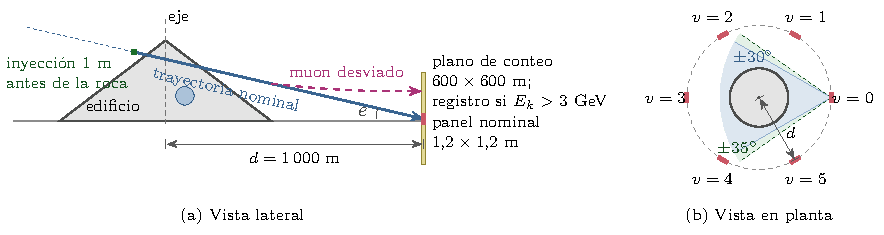
\includegraphics{fig3-3_geometria_observacion.pdf}
\caption[Geometría de observación de la simulación]{Geometría de observación de la campaña definitiva. (a)~Vista lateral: edificio cónico, panel detector nominal de $1{,}2\times1{,}2$~m a la distancia $d$ del eje, plano de conteo de $600\times600$~m centrado en el panel, trayectoria nominal con el punto de inyección situado 1~m antes de la entrada en la roca y trayectoria de un muon desviado por dispersión múltiple. (b)~Vista en planta: seis posiciones del detector, separadas 60°, ventana de conteo de $\pm30^{\circ}$ y ventana de generación de $\pm35^{\circ}$ de la vista~0. Esquema sin escala. Fuente: elaboración propia a partir de la receta operativa.}
\label{fig:geometria-observacion}
\end{figure}

El registro, en cambio, se hizo sobre un plano de conteo mucho mayor que el panel: un cuadrado de $600\times600$~m centrado en él. Cuando el muon primario alcanza ese plano con energía cinética superior a 3~GeV, se calculan la elevación y el acimut de su dirección de llegada y se le asigna el píxel correspondiente de la malla angular. La razón de esta separación es la dispersión coulombiana múltiple \parencite{lynch1991}: a lo largo de cientos de metros de roca y de aire, los muones de pocos GeV se desvían decenas de metros de su trayectoria nominal, de modo que una superficie de registro del tamaño del panel perdería una fracción de los muones generados sobre él que depende de su energía. El umbral de 3~GeV elimina, además, los muones blandos dispersados cuya contribución dependía del tamaño del plano. Debe subrayarse que la independencia del conteo respecto del tamaño del plano, que se comprobó en los ensayos de la sección~\ref{subsec:met-verificacion}, es una convergencia del muestreo para una fuente restringida al panel nominal: no demuestra que la imagen sea la de un detector físico de 1,2~m expuesto a una fuente espacialmente amplia.

La malla angular sustituyó a la convención histórica del conjunto inicial, que asignaba cada dirección al más cercano de 256 centros equiespaciados entre $-30^{\circ}$ y $30^{\circ}$, de modo que los dos intervalos extremos tenían la mitad del ancho de los interiores. En la convención adoptada, el acimut relativo se divide en 256 intervalos iguales delimitados por bordes explícitos, mientras que en elevación se conservaron los 256 centros entre 2° y 47° de la convención histórica. Cada histograma se registró en tres versiones complementarias: con el umbral de 3~GeV, que constituye la referencia; sin umbral, y por dirección nominal de generación, esta última usada para contar exactamente $N_{\mathrm{nom},v}$. Ningún evento recibió un peso estadístico: todos tuvieron peso unitario, la dependencia direccional quedó contenida en el muestreo de filas y la exposición convencional en la \cref{eq:fuente-t}.

\subsection{Verificación de la cadena de simulación}
\label{subsec:met-verificacion}

La verificación se organizó siguiendo los eslabones de la cadena: el generador de muones, las geometrías y su corrección, la malla angular, el observable y su normalización, el piloto con la receta de producción y, finalmente, la calidad de las referencias de la campaña. La \cref{tab:verificacion} resume cada comprobación con su procedimiento, su criterio y su estado. Dos precisiones delimitan su alcance. La primera es que la bitácora del conjunto inicial se reconstruyó después de su campaña a partir de registros primarios, de modo que los procedimientos anteriores a la revisión técnica se describen con esa trazabilidad retrospectiva. La segunda es que varias comprobaciones se diseñaron y ejecutaron sobre el motor analítico, y su validez no se transfiere automáticamente al transporte con Geant4. Los resultados de todas ellas se presentan en el capítulo~\ref{chap:resultados}.

\begin{table}[htbp]
\centering
\caption[Comprobaciones de la cadena de simulación]{Comprobaciones de la cadena de simulación: procedimiento, criterio y estado. Los resultados se presentan en el capítulo~\ref{chap:resultados}. Fuente: elaboración propia a partir del repositorio de referencia.}
\label{tab:verificacion}
\small
\begin{tabularx}{\linewidth}{@{}>{\raggedright\arraybackslash}p{2.6cm}>{\raggedright\arraybackslash}X>{\raggedright\arraybackslash}p{3.4cm}>{\raggedright\arraybackslash}p{1.8cm}@{}}
\toprule
Eslabón & Procedimiento & Criterio & Estado \\
\midrule
Generador & muestreador y tablas frente a la parametrización de Guan & residuo relativo máximo $<10\,\%$; reproducción de $S_0$ & ejecutado \\
Generador & muestra de EcoMug frente a la parametrización de Guan & sin criterio; diferencia declarada como hipótesis & ejecutado \\
Geometrías & auditoría analítica y control geométrico de la regla B1 & \cref{tab:control-t} & ejecutado \\
Corrección & piloto A/B en geo-train-06 & partición de la \cref{eq:piloto} & ejecutado \\
Corrección & segundo ensayo con primarios compartidos y complemento dirigido & protocolo de la dirección; resultado inconcluso admitido & ejecutado \\
Malla angular & integración en el supercomputador con 1\,000 primarios & metadatos, histograma, registro y código de salida & ejecutado \\
Observable & planos de conteo, aire previo, bordes y asíntota & fijados antes de ejecutar & ejecutado \\
Observable & equivalencia con un panel físico & intervalo simultáneo en $[0{,}95;\,1{,}05]$ & no ejecutado \\
Piloto & seis vistas de geo-train-06 con la receta de producción & bordes con $\alpha=0{,}05/6$ & ejecutado \\
Campaña & integridad, bordes y suficiencia en roca & \cref{eq:bordes} y~\cref{eq:roca} & ejecutado \\
Reproducción & evaluación desde los píxeles y regeneración de pares & huellas de archivo y de contenido & ejecutado \\
\bottomrule
\end{tabularx}
\end{table}

\paragraph{Generador de muones.}
El muestreador del motor analítico se contrastó con la parametrización de \textcite{guan2015muonflux} mediante una muestra de $10^7$ muones. Se compararon el espectro de energía, en 40 intervalos logarítmicos entre 0,5 y 100~GeV, y la distribución del ángulo cenital $\zeta$, en 35 intervalos de $\cos\zeta$ entre 0° y 70°, y la validación se consideró superada solo si el residuo relativo máximo fue inferior al 10\,\% en ambas distribuciones. La muestra de EcoMug se comparó con la misma parametrización incorporando el factor de aceptancia $\cos\zeta$, necesario porque EcoMug genera el flujo que atraviesa una superficie horizontal; esta segunda comparación no tuvo un criterio de aprobación, porque EcoMug implementa su propia parametrización y una diferencia moderada entre modelos es esperable. Para la receta definitiva se recalculó, además, la escala $S_0$ directamente desde la parametrización de Guan y se comprobó, con una prueba de bondad de ajuste $\chi^2$ de 255 grados de libertad, que el generador reproducía la distribución de las direcciones por filas de elevación.

\paragraph{Transporte y normalización de cielo abierto en el motor analítico.}
Sobre el motor analítico se aplicaron cuatro pruebas físicas: la transmisión a través del edificio homogéneo frente a un cálculo teórico independiente, con error relativo máximo inferior a 0,15; la sensibilidad al contraste de una cavidad conocida de 40~m de radio y densidad nula, cuyo espesor másico y transmisión debían coincidir con los teóricos con el mismo error; la dispersión de Poisson de los conteos sobre 400 réplicas, con índice de dispersión medio a menos de 0,05 de la unidad y menos del 10\,\% de los píxeles fuera de la banda bilateral del 95\,\%; y la exactitud de la tabla de interpolación del flujo frente a la integración directa, con error relativo inferior a 0,01.

\paragraph{Corrección de la geometría geo-train-06.}
La auditoría del catálogo mostró que en seis escenarios las anomalías se superponían entre sí o sobresalían del edificio, y que Geant4 había emitido las advertencias correspondientes durante la campaña del conjunto inicial. Como en una región compartida por dos volúmenes hermanos Geant4 no define qué material se atraviesa, se diseñó una corrección y se ensayó primero en geo-train-06, donde un conducto y un cuerpo denso se intersectan. El diagnóstico previo estimó la intersección con $4\times10^6$ muestras uniformes en la caja envolvente común de ambas anomalías y verificó la contención del cuerpo denso sobre una parametrización de su superficie con paso angular de 0,25°. La corrección adoptada, denominada B1, define la región material que corresponde a cada anomalía mediante la \cref{eq:b1},
\begin{equation}
\mathcal{R}_i=\left(A_i\cap\mathcal{K}\right)\setminus\bigcup_{j>i}A_j ,
\label{eq:b1}
\end{equation}
donde $A_i$ es el sólido de la anomalía de índice $i$ en el orden de declaración, $\mathcal{K}$ es el cono del edificio y $\mathcal{R}_i$ es la región que recibe finalmente la densidad de la anomalía $i$. Cada anomalía se recorta al edificio y cede a las anomalías declaradas después la región que comparte con ellas. La regla coincide con la que ya aplicaba el motor analítico, de modo que ambos motores pasan a representar el mismo campo de materiales, y no modifica ningún parámetro publicado del catálogo. El algoritmo~\ref{alg:b1} muestra su implementación con sólidos booleanos de Geant4. El recorte al edificio se realizó contra un cono auxiliar interior al edificio por un margen de 1~mm, para evitar superficies coincidentes con el volumen madre; por ese margen, la correspondencia con el campo analítico no es exacta en las fronteras. Se consideraron y descartaron dos alternativas: dar prioridad al conducto, que introducía una divergencia nueva con el motor analítico, y desplazar el cuerpo denso, que alteraba el escenario físico publicado.

\begin{algorithm}[htbp]
\caption{Construcción de los volúmenes de las anomalías con la regla B1}
\label{alg:b1}
\begin{algorithmic}[1]
\Require sólidos de las anomalías $A_1,\dots,A_m$ en el orden de declaración; cono del edificio $\mathcal{K}$; cono auxiliar $\mathcal{K}^{-}$, interior a $\mathcal{K}$ por 1~mm
\Ensure volúmenes colocados que realizan las regiones $\mathcal{R}_1,\dots,\mathcal{R}_m$ de la \cref{eq:b1}
\For{$i \gets 1$ \textbf{hasta} $m$}
  \State $S \gets A_i$
  \If{una prueba suficiente no certifica que $A_i$ está contenida en $\mathcal{K}$}
    \State $S \gets S \cap \mathcal{K}^{-}$ \Comment{intersección booleana}
  \EndIf
  \For{$j \gets i+1$ \textbf{hasta} $m$}
    \If{las cajas envolventes de $A_i$ y $A_j$ se superponen}
      \State $S \gets S \setminus A_j$ \Comment{sustracción booleana}
    \EndIf
  \EndFor
  \If{$S$ no es vacío}
    \State colocar $S$ como volumen hijo de $\mathcal{K}$ con la densidad de la anomalía $i$
  \Else
    \State registrar en el diagnóstico que la anomalía $i$ no se coloca
  \EndIf
\EndFor
\end{algorithmic}
\end{algorithm}

La corrección se evaluó comparando dos ejecutables compilados desde la misma base de código: la variante~A, que conserva la geometría original como referencia de diagnóstico, y la variante~B, que incorpora la regla B1. Primero se ejecutó un control geométrico en cuatro tareas, cuyo diseño y criterios resume la \cref{tab:control-t}. La primera tarea buscó superposiciones en las 19 geometrías, las 6 vistas y ambas variantes; las siguientes contrastaron la construcción de geo-train-06 con el motor analítico mediante sondeos puntuales, volúmenes y cortes, y la última comprobó que una simulación ordinaria de la variante~B terminara sin advertencias geométricas. Los volúmenes de las cuatro intersecciones del catálogo se contrastaron, además, en la revisión de la dirección, mediante una integración numérica independiente por cuadratura adaptativa. Ninguno de estos controles mide el efecto de la corrección sobre los conteos, que es el objeto de los ensayos siguientes.

\begin{table}[htbp]
\centering
\caption[Diseño del control geométrico de la corrección B1]{Diseño del control geométrico de la corrección B1. A: variante con la geometría original; B: variante con la regla B1 (\cref{eq:b1}). Fuente: elaboración propia a partir de la entrega del ensayo de corrección.}
\label{tab:control-t}
\small
\begin{tabularx}{\linewidth}{@{}lXX@{}}
\toprule
Tarea & Procedimiento & Criterio \\
\midrule
T1 & búsqueda de superposiciones con $10^5$ puntos por volumen y tolerancia nula en 19 geometrías, 6 vistas y 2 variantes (228 ejecuciones) & B sin superposiciones; A con superposiciones solo en las geometrías señaladas por la auditoría \\
T2 & en geo-train-06, vista~0: sondeos puntuales del navegador, volúmenes de las anomalías con $10^7$ muestras y dos cortes frente al motor analítico & sondeos coincidentes; volúmenes dentro de tres errores estándar combinados; discrepancias de corte explicadas como borde o como clase aire \\
T3 & mapas de material y de discrepancia en los dos cortes & inspección visual \\
T4 & simulación ordinaria de geo-train-06, vista~0, con $10^4$ eventos & B completa, sin advertencias geométricas, con histograma no vacío y totales coherentes; A como referencia \\
\bottomrule
\end{tabularx}
\end{table}

\paragraph{Ensayo piloto de la corrección.}
El ensayo piloto comparó las variantes A y B sobre la vista~0 de geo-train-06, con $10^6$ eventos por simulación, tres semillas y las mismas tablas, física y recursos en ambas variantes. Antes de enviar las simulaciones se registraron en un prerregistro cinco regiones de interés derivadas exclusivamente de la geometría, por trazado de rayos sobre la rejilla angular y nunca a partir de las imágenes medidas: la intersección entre las anomalías, el conducto exclusivo, el cuerpo denso exclusivo, la roca sin anomalías y el cielo, estas dos últimas como controles. El mismo prerregistro acotó el efecto máximo esperado, $\Delta_{\max}$, como la diferencia de conteos entre suponer que el cuerpo denso ocupa la intersección y suponer que la ocupa el conducto, y anticipó que, con ese número de eventos, la región de intersección no tendría potencia suficiente para distinguir las variantes. Para cada región y semilla $s$ se definieron la diferencia emparejada, su media y su error estándar, y los resultados posibles se particionaron de antemano en cuatro casos según la \cref{eq:piloto}:
\begin{subequations}\label{eq:piloto}
\begin{align}
d_s &= C_{B,s}-C_{A,s}, \qquad \bar d=\frac{1}{3}\sum_{s=1}^{3}d_s, \qquad \mathrm{EE}=\frac{\mathrm{SD}(d_s)}{\sqrt{3}}, \label{eq:piloto-dif}\\
\mathrm{EE}_{\mathrm{prev}} &= \sqrt{2N_{\mathrm{B1}}/3}, \label{eq:piloto-ee}\\
\text{resultado} &=
\begin{cases}
\text{inconcluso}, & \mathrm{EE}_{\mathrm{prev}}>|\Delta_{\max}|,\\
\text{nulo}, & |\bar d|\le 2\,\mathrm{EE}_{\mathrm{prev}},\\
\text{efecto presente}, & |\bar d|>2\,\mathrm{EE}_{\mathrm{prev}}\ \text{y compatible con}\ \Delta_{\max},\\
\text{discordante}, & |\bar d|>2\,\mathrm{EE}_{\mathrm{prev}}\ \text{e incompatible con}\ \Delta_{\max}.
\end{cases} \label{eq:piloto-decision}
\end{align}
\end{subequations}
En estas expresiones, $C_{V,s}$ es el conteo total dentro de la región para la variante $V$ y la semilla $s$; $\mathrm{SD}(d_s)$ es la desviación estándar de las tres diferencias; $\mathrm{EE}$ es el error estándar observado, y $\mathrm{EE}_{\mathrm{prev}}$ es el error estándar previsto a partir del conteo esperado por simulación bajo la regla B1, $N_{\mathrm{B1}}$. Los tres últimos casos de la \cref{eq:piloto-decision} solo se aplican cuando $\mathrm{EE}_{\mathrm{prev}}\le|\Delta_{\max}|$: un resultado inconcluso indica que la estadística planeada no tenía, de partida, capacidad para separar el valor nulo de $\Delta_{\max}$, y no debe interpretarse como evidencia de que las variantes sean equivalentes; un resultado nulo, en cambio, se obtiene con potencia adecuada; una diferencia es compatible con $\Delta_{\max}$ cuando tiene su mismo signo y no lo supera ampliamente en magnitud; y un resultado discordante exige investigar el procedimiento antes de cualquier conclusión. El umbral de dos errores estándar es una regla heurística y no un intervalo de Student, pues con tres semillas el valor crítico exacto sería $t_{0{,}975;\,2}\approx4{,}303$. Las regiones de control debían mostrar diferencias compatibles con cero, lo que permite descartar diferencias espurias del procedimiento.

\paragraph{Segundo ensayo con correspondencia de primarios.}
Usar semillas iguales no garantiza que las variantes transporten los mismos muones, porque cambiar la geometría altera la secuencia de números aleatorios. Por ello, la dirección del proyecto definió un segundo ensayo en el que ambas variantes leen una misma lista de muones primarios generada de antemano y registran, para cada primario, si fue detectado, en qué píxel y si atravesó la región original de la intersección. Su primera etapa comprendió las geometrías geo-train-06 y geo-train-01, esta última sin anomalías como control, en su vista~0, con tres réplicas de la comparación A/B y una repetición técnica A/A, en 13 simulaciones de $10^5$ primarios con trazabilidad individual. Un complemento dirigido, con doce trayectorias que atraviesan la región compartida y tres semillas por variante, comprobó a qué material asigna cada variante esa región. La segunda etapa, regida por un protocolo revisado, fijó de antemano un tamaño de $2{,}4\times10^{7}$ pares principales de primarios, con 55 simulaciones y $4{,}87\times10^{7}$ transportes en total incluidos los controles; un margen operativo ligado al ruido de conteo de la región de interés; un intervalo de confianza conservador de al menos 95\,\% construido con límites binomiales exactos, y la admisión explícita de un resultado inconcluso, sin ampliación automática del tamaño.

\paragraph{Malla angular.}
La revisión del registro angular cuantificó la discretización de la convención histórica y motivó la adopción de la malla de intervalos iguales de la \cref{tab:geant4}. Su integración en la aplicación de transporte se comprobó en el supercomputador con una simulación de 1\,000 primarios, revisando los metadatos, el histograma, el registro de ejecución y el código de salida, antes de cualquier producción con la nueva malla.

\paragraph{Diagnóstico del observable y de la normalización.}
Para fijar el observable de la campaña se ejecutaron en el supercomputador cuatro controles cortos sobre la vista~0 de la geometría homogénea geo-train-01, cada uno con su pregunta, su comparación y su criterio de resultado establecidos antes de la ejecución. Un único plano de 1\,200~m registró a la vez cuadrados anidados de 1,2, 100, 300 y 600~m de lado con los mismos muones, de modo que la razón entre planos es una fracción binomial anidada. El primer control comparó, para varios umbrales de energía cinética y tres puntos de inyección, la razón de conteos entre los planos de 100 y 600~m por bandas de espesor másico de roca, con el criterio de una razón de al menos 0,98 en todas las bandas; el segundo midió la eficiencia de cielo abierto para decidir si el muon debía atravesar el aire previo; el tercero midió la desviación de las filas y columnas de borde frente al interior para varios márgenes angulares de generación; y el cuarto comparó los planos de 600 y 1\,200~m para comprobar la asíntota. Un quinto control, que habría comparado la imagen del estimador con la de un panel físico expuesto a una fuente espacialmente amplia, quedó diseñado con un criterio de equivalencia por intervalos simultáneos, pero no se ejecutó: su costo era elevado y el alcance adoptado no exige equivalencia instrumental.

\paragraph{Piloto de seis vistas.}
Con la receta de producción fijada, se ejecutó un piloto sobre las seis vistas de geo-train-06, con $2{,}11\times10^{8}$ primarios por vista en seis bloques. El piloto aplicó el criterio de bordes que se describe a continuación, con un error familiar del 5\,\% repartido entre sus seis vistas, y registró los mismos indicadores descriptivos de roca. Se evaluó una sola vez, con el número de primarios fijado, y sus resultados sirvieron para dimensionar el presupuesto de la campaña; sus histogramas no se sumaron a las referencias finales.

\paragraph{Criterios de calidad de la campaña.}
Las referencias de la campaña se evaluaron con tres criterios registrados antes del envío. El primero, de integridad, exigió exactamente 114 referencias compatibles, con el número de primarios, las semillas, la receta, las geometrías y las tablas del manifiesto, conteos enteros sin saturación y procedencia verificable; un error técnico impedía aceptar la vista. El segundo evaluó la respuesta en los bordes de la ventana frente a una referencia ideal de la fuente sin transporte. Para cada vista se definieron quince regiones de borde, formadas por las cinco columnas extremas de cada lado y las cinco filas superiores, restringidas al cielo entre 30° y 42° de elevación en el caso de las columnas, y una región interior con las columnas 20 a 235 en la misma banda de cielo. La respuesta de cada región se contrastó con la de la región interior según la \cref{eq:bordes}:
\begin{subequations}\label{eq:bordes}
\begin{align}
\hat p_r &= \frac{C_r}{N_v}, \label{eq:bordes-p}\\
\varepsilon_r &= \frac{\hat p_r-p^{\mathrm{ideal}}_r}{p^{\mathrm{nom}}_r}, \label{eq:bordes-e}\\
\Delta_r &= \varepsilon_r-\varepsilon_{\mathrm{int}}, \qquad \text{equivalente si}\ \left[\Delta_r^{-};\,\Delta_r^{+}\right]\subset\left[-0{,}01;\,0{,}01\right], \label{eq:bordes-d}
\end{align}
\end{subequations}
donde $C_r$ es el conteo de la región $r$ en la referencia; $N_v$ es el número de primarios de la vista; $\hat p_r$ es la probabilidad estimada de que un primario sea registrado en la región; $p^{\mathrm{ideal}}_r$ es la probabilidad de que la fuente ideal, sin transporte, produzca un primario con dirección en la región y energía cinética superior al umbral; $p^{\mathrm{nom}}_r$ es la probabilidad de que la dirección nominal de un primario caiga en la región; $\varepsilon_r$ es la respuesta relativa de la región y $\varepsilon_{\mathrm{int}}$ la de la región interior; y $\left[\Delta_r^{-};\,\Delta_r^{+}\right]$ es el intervalo del contraste. La resta de $p^{\mathrm{ideal}}_r$ ajusta el cambio del espectro con la elevación, y la tolerancia de 0,01 equivale a $\pm1$ punto porcentual de probabilidad de registro por inyección nominal. Cada probabilidad se trató como una proporción binomial de $N_v$ historias independientes, con a lo sumo una llegada registrada por primario, y se acotó con intervalos de \textcite{clopper1934}; con una corrección de Bonferroni \parencite{dunn1961}, el error familiar de 0,05 se repartió entre las 114 vistas y, dentro de cada vista, entre sus dieciséis probabilidades, y los extremos del contraste se obtuvieron restando los extremos de los intervalos, una cota simultánea conservadora que no supone independencia entre regiones.

El tercer criterio describió la suficiencia del conteo en la roca. Se predefinieron, sin observar los conteos, regiones de interés de $4\times4$ píxeles cuyo espesor másico nominal en el cono homogéneo, calculado por marcha de rayos de 2~m con el procedimiento del motor analítico de la sección~\ref{subsec:met-campana}, quedara entre $3\times10^{4}$ y $10^{5}$~g\,cm$^{-2}$. Esas máscaras ignoran las anomalías, que sí se transportan, y son comunes a las seis vistas de cada geometría por la simetría circular del cono homogéneo; contienen entre 150 y 244 regiones por geometría. Para cada vista se calculó el indicador de la \cref{eq:roca},
\begin{equation}
F_v=\frac{1}{M_v}\sum_{m=1}^{M_v}\mathbf{1}\!\left[C_{v,m}\geq100\right],
\label{eq:roca}
\end{equation}
donde $M_v$ es el número de regiones de roca de la vista, $C_{v,m}$ es la suma de los conteos de la referencia en la región $m$ y $\mathbf{1}[\cdot]$ es la función indicadora. La meta descriptiva, $F_v\geq0{,}90$, se acompañó de la mediana y el percentil 10 de los conteos por región. Cien cuentas representan aproximadamente un 10\,\% de ruido relativo de conteo en la región agregada, sin incluir la incertidumbre del modelo; el indicador no constituye una precisión por píxel, un criterio para toda la roca ni una garantía sobre las tasas verdaderas. El acuerdo previo con la dirección estableció que una vista por debajo de la meta se conservaría y se reportaría, sin aumentar el número de primarios, descartar imágenes ni modificar la regla después de conocer los resultados.

\subsection{Ejecución de la campaña y formación de imágenes}
\label{subsec:met-campana}

La campaña de transporte simuló las 114 vistas del catálogo en el supercomputador de la universidad (sección~\ref{subsec:met-entorno}), con un número fijo de $3{,}44\times10^{8}$ primarios por vista, para un total de $3{,}9216\times10^{10}$. Cada vista se dividió en nueve bloques, ocho de 38\,222\,223 primarios y uno de 38\,222\,216, de modo que la campaña comprendió 1\,026 bloques definidos en un manifiesto congelado antes del envío. Para que cualquier bloque pudiera repetirse de forma independiente, su semilla se derivó de manera determinista mediante la \cref{eq:semilla-campana},
\begin{equation}
s(g,v,b)=20261002\cdot10^{6}+6\cdot10^{5}+g\cdot10^{4}+v\cdot10^{2}+b ,
\label{eq:semilla-campana}
\end{equation}
donde $s$ es la semilla del bloque, $g\in\{0,\dots,18\}$ la posición de la geometría en el orden alfabético del catálogo, $v\in\{0,\dots,5\}$ la vista y $b\in\{0,\dots,8\}$ el índice del bloque. Las semillas son nuevas respecto de las del piloto, y ninguna se repite.

La ejecución se automatizó con un procedimiento idempotente, descrito en el algoritmo~\ref{alg:campana}, que tolera interrupciones y repeticiones sin corromper los resultados. En cada pasada, el procedimiento compara el manifiesto con los bloques ya publicados, omite los bloques con un trabajo en curso o con un intento previo sin conciliar y envía los bloques pendientes al gestor de trabajos. Cada trabajo simula su bloque en un directorio temporal y, al terminar, el bloque se publica solo después de verificar la copia y la huella SHA-256 \parencite{nist2015} de sus archivos frente al recibo, de modo que un bloque incompleto o alterado nunca llega al directorio de publicación. Un trabajo fallido se concilia con los registros del gestor antes de cualquier reintento, y ningún registro se borra para forzar un envío. La receta, el manifiesto y las herramientas se verificaron por sus huellas al inicio de cada trabajo, y la copia de trabajo no se modificó durante la campaña.

\begin{algorithm}[htbp]
\caption{Ejecución idempotente de la campaña por bloques}
\label{alg:campana}
\begin{algorithmic}[1]
\Require manifiesto congelado de bloques $\{(g,v,b,s,N_b)\}$; receta y herramientas con sus huellas; directorios temporal y de publicación
\Ensure un bloque publicado y verificado por cada fila del manifiesto
\Function{Pasada}{}
  \State verificar las huellas del manifiesto, la receta y las herramientas
  \State $\mathcal{F} \gets$ filas del manifiesto sin bloque publicado, excluidas las que tienen un trabajo en curso o un intento previo sin conciliar
  \For{cada fila $(g,v,b,s,N_b)$ de $\mathcal{F}$, dentro del cupo disponible}
    \State enviar un trabajo \Call{Simular}{$g,v,b,s,N_b$}
  \EndFor
\EndFunction
\Function{Simular}{$g,v,b,s,N_b$}
  \State transportar $N_b$ primarios de la vista $v$ de la geometría $g$ con semilla $s$ (\cref{eq:semilla-campana}) en un directorio temporal
  \State escribir los histogramas con y sin umbral, el de direcciones nominales, los metadatos y el recibo con sus huellas
  \If{la copia y las huellas se verifican frente al recibo}
    \State publicar el bloque mediante un renombrado atómico
  \Else
    \State conservar el intento y registrarlo para su conciliación
  \EndIf
\EndFunction
\end{algorithmic}
\end{algorithm}

Concluida la campaña, los bloques se fusionaron por vista con un contrato estricto: la fusión exige exactamente los nueve bloques de la vista, con las semillas, los primarios y las huellas de receta, geometría, ejecutable y tablas del manifiesto, y rechaza cualquier configuración incompatible. Como los conteos son aditivos, la fusión es una suma entera exacta de los tres histogramas de cada bloque. Para cada vista se registraron el histograma fusionado, los primarios transportados, el número de direcciones nominales en la ventana, los muones registrados con y sin umbral, la exposición convencional de la \cref{eq:fuente-t}, las semillas de los bloques y las huellas de entrada y de salida. Por último, cada histograma con umbral se exportó a un formato binario común, con un arreglo de conteos de enteros sin signo de 32 bits y los bordes y centros explícitos de la malla angular en acimut y en elevación, y se comprobó que la exportación conservara exactamente los conteos y las coordenadas del histograma.

Cada imagen resultante es un arreglo de $256\times256$ píxeles ordenado por elevación y acimut. La elevación cubre de 2° a 47° sobre la horizontal y el acimut relativo, de $-30^{\circ}$ a $30^{\circ}$ alrededor de la dirección de observación del detector hacia el eje del cono. El valor de un píxel es un conteo adimensional: el número de muones primarios, de los $3{,}44\times10^{8}$ generados para la vista, que alcanzaron el plano de conteo con energía cinética superior a 3~GeV y con dirección de llegada en esa celda angular.

Ese conteo debe distinguirse de dos magnitudes derivadas que la muografía por transmisión utiliza para interpretar las imágenes: la opacidad y la transmisión \parencite{lesparre2010}. En este trabajo ambas se calcularon con el motor analítico, que intervino en la cadena como antecedente de validación, en la construcción de las tablas del generador, en la selección de las regiones de roca y en las regiones de interés de los ensayos. El motor traza cada dirección a través del campo de densidades y obtiene sucesivamente la opacidad, la energía mínima que un muon necesita para atravesarla, la transmisión y el conteo esperado, según la \cref{eq:analitico}:
\begin{subequations}\label{eq:analitico}
\begin{align}
X &= \sum_{m}\rho(\mathbf{r}_m)\,\Delta\ell, \label{eq:opacidad}\\
E_{\min}(X) &= \frac{a}{b}\left(\mathrm{e}^{bX}-1\right), \label{eq:emin}\\
T &= \frac{\Phi_{\mathrm{int}}\!\left(E_{\min}(X),\zeta\right)}{\Phi_{\mathrm{int}}\!\left(E_{\min}(X_{\mathrm{aire}}),\zeta\right)}, \qquad \cos\zeta=\sin e, \label{eq:transmision}\\
\lambda &= \Phi_{\mathrm{int}}\!\left(E_{\min}(X),\zeta\right)A\,\Delta\Omega\,t, \qquad \Delta\Omega=\Delta\alpha\,\Delta e\,\cos e. \label{eq:lambda}
\end{align}
\end{subequations}
En la \cref{eq:opacidad}, $X$ es la opacidad o espesor másico, en g\,cm$^{-2}$; $\rho(\mathbf{r}_m)$ es la densidad, en g\,cm$^{-3}$, en el punto $\mathbf{r}_m$ de la marcha del rayo, y $\Delta\ell=2{,}0$~m es el paso de la marcha, expresado en centímetros en el cálculo; el trayecto incluye el aire hasta una longitud máxima de 3\,000~m. En la \cref{eq:emin}, $E_{\min}$ es la energía mínima en GeV según la aproximación de frenado continuo en roca estándar, con $a=2{,}17\times10^{-3}$~GeV\,cm$^{2}$\,g$^{-1}$ y $b=4{,}0\times10^{-6}$~cm$^{2}$\,g$^{-1}$ \parencite{groom2001,pdg2022}. En la \cref{eq:transmision}, $T$ es la transmisión, $\Phi_{\mathrm{int}}(E,\zeta)$ es el flujo integral de muones con energía superior a $E$ según \textcite{guan2015muonflux}, $\zeta$ el ángulo cenital, $e$ la elevación y $X_{\mathrm{aire}}$ la opacidad de la misma trayectoria solo en aire. En la \cref{eq:lambda}, $\lambda$ es el conteo esperado del píxel; $A=1{,}44\times10^{4}$~cm$^{2}$ es el área del detector; $\Delta\alpha$ y $\Delta e$ son los pasos angulares de la rejilla en acimut y elevación, en radianes, y $t$ es la exposición en segundos. El motor analítico supone una aceptancia plana, sin eficiencia angular ni fondo instrumental, y no modela la dispersión múltiple, las fluctuaciones de la pérdida de energía ni la respuesta del detector; esas ausencias motivaron el transporte con Geant4.

\subsection{Construcción de pares de baja y alta estadística}
\label{subsec:met-pares}

Para obtener imágenes de baja estadística sin repetir el transporte, las entradas se construyeron reduciendo los conteos de cada referencia. La referencia de alta estadística de la vista $v$ es su imagen exportada, $C^{\mathrm{ref}}_v$, que contiene el 100\,\% de los muones registrados. Cada entrada de baja estadística se obtuvo por adelgazamiento binomial de esos conteos, píxel a píxel, lo que equivale a conservar cada muon registrado de forma independiente con probabilidad $f$; es el submuestreo previsto en el plan de trabajo, empleado también en otros estudios de mejora de imágenes muográficas \parencite{odonnell2025particles}. La \cref{eq:pares} define la operación y sus dos primeros momentos condicionales:
\begin{subequations}\label{eq:pares}
\begin{align}
C^{\mathrm{low}}_{v,f,k}(q) &\sim \mathrm{Bin}\!\left(C^{\mathrm{ref}}_v(q),\,f\right), \label{eq:adelgazamiento}\\
\mathrm{E}\!\left[C^{\mathrm{low}}\mid C^{\mathrm{ref}}\right] &= f\,C^{\mathrm{ref}}, \label{eq:pares-media}\\
\mathrm{Var}\!\left[C^{\mathrm{low}}\mid C^{\mathrm{ref}}\right] &= f(1-f)\,C^{\mathrm{ref}}, \label{eq:pares-varianza}
\end{align}
\end{subequations}
donde $q$ indexa el píxel, $f\in\{0{,}50;\ 0{,}10;\ 0{,}05;\ 0{,}01\}$ es la fracción conservada y $k=1,\dots,20$ indexa la realización. Las entradas se almacenaron como enteros sin signo de 32 bits, sin recorte, sin suavizado y sin normalización por imagen, y se comprobó que ningún conteo reducido superara el de su referencia.

La elección del adelgazamiento binomial se justifica por una propiedad de los procesos de Poisson: si los muones registrados forman un proceso de Poisson de tasa constante, conservar cada uno de forma independiente con probabilidad $f$ produce otro proceso de Poisson con tasa $f$ veces menor \parencite{kingman1992}. Bajo ese supuesto, una entrada con fracción $f$ tiene la misma estadística que una exposición convencional $f\,T_v$ del mismo observable, con la ventaja de que se obtiene de los mismos muones ya transportados. El algoritmo~\ref{alg:pares} resume la construcción. Los generadores de las realizaciones se derivaron de forma determinista de una semilla maestra de valor 20260805 y de la geometría, la vista, la fracción y la realización. Cada vista produjo un archivo con su referencia, de dimensión $256\times256$; sus entradas, de dimensión $4\times20\times256\times256$; las fracciones y las coordenadas angulares, es decir, 80 pares por vista, 114 archivos y 9\,120 pares en total.

\begin{algorithm}[htbp]
\caption{Construcción de los pares de baja y alta estadística de una vista}
\label{alg:pares}
\begin{algorithmic}[1]
\Require referencia $C^{\mathrm{ref}}_v$ de la vista $v$ de la geometría $g$, con sus coordenadas; fracciones $\mathcal{F}=\{0{,}50;\,0{,}10;\,0{,}05;\,0{,}01\}$; número de realizaciones $K=20$; semilla maestra 20260805
\Ensure archivo de pares de la vista, con 80 entradas y su inventario de huellas
\For{cada fracción $f_i \in \mathcal{F}$}
  \For{$k \gets 1$ \textbf{hasta} $K$}
    \State derivar un generador independiente a partir de la semilla maestra y de $(g, v, i, k)$
    \State $C^{\mathrm{low}}_{v,f_i,k} \gets \mathrm{Bin}(C^{\mathrm{ref}}_v, f_i)$ píxel a píxel (\cref{eq:adelgazamiento})
    \State comprobar que $C^{\mathrm{low}}_{v,f_i,k}\le C^{\mathrm{ref}}_v$ en todos los píxeles
  \EndFor
\EndFor
\State guardar la referencia, las entradas, las fracciones y las coordenadas en el archivo de pares de la vista
\State registrar la huella del archivo y las huellas de contenido de sus arreglos
\end{algorithmic}
\end{algorithm}

La construcción introduce dependencias que deben tenerse en cuenta al interpretar los resultados. Los muones de cada entrada son un subconjunto de los de su referencia, de modo que entrada y referencia no son independientes, y las veinte realizaciones de una vista comparten la misma referencia finita; no son veinte simulaciones independientes de $f\,N_v$ primarios. La referencia, a su vez, no está libre de ruido: es una única realización estocástica del transporte de $3{,}44\times10^{8}$ primarios y conserva su propio ruido de conteo, cuya magnitud relativa en un píxel con $C^{\mathrm{ref}}$ muones es del orden de $1/\sqrt{C^{\mathrm{ref}}}$. No se dispuso de una referencia de mayor exposición con la cual acotar ese ruido. Además, la equivalencia entre la fracción $f$ y una exposición convencional $f\,T_v$ hereda los supuestos del flujo y del área de detección de la sección~\ref{subsec:met-fuente}.
% PENDIENTE (discutir con la dirección): cuantificación del ruido residual de la
% referencia en los píxeles de roca, más allá del indicador agregado de la ecuación
% de suficiencia en roca.

La \cref{fig:pares} ilustra el resultado para la vista~0 de geo-train-08: la referencia y las entradas con fracciones 0,50, 0,10, 0,05 y 0,01, representadas en una escala logarítmica común y sin renormalizar por la fracción. La degradación progresiva de la imagen al reducir la fracción muestra el problema que los modelos de los objetivos siguientes buscan corregir.

\begin{figure}[htbp]
\centering
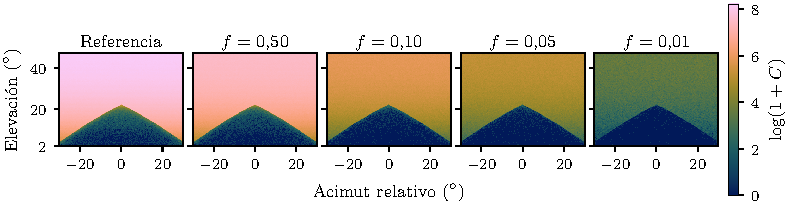
\includegraphics{fig3-4_ejemplo_pares.pdf}
\caption[Ejemplo de un par de baja y alta estadística]{Imágenes de la vista~0 de geo-train-08: referencia ($3{,}44\times10^{8}$ primarios) y primera realización de las entradas obtenidas por adelgazamiento binomial con fracciones 0,50, 0,10, 0,05 y 0,01, en la escala común $\log(1+C)$, donde $C$ es el conteo del píxel. Fuente: elaboración propia a partir del archivo de pares de la campaña de 114 vistas, cuyas huellas de contenido se verificaron antes de generar la figura.}
\label{fig:pares}
\end{figure}

El adelgazamiento binomial depende de la implementación del generador de números aleatorios de la biblioteca numérica, de modo que reconstruir los pares con otra versión puede producir realizaciones distintas; por ello, el procedimiento fija la versión 2.4.4 de NumPy. Además, la huella de un archivo comprimido depende de la versión de la biblioteca de compresión con que se escribió, aunque su contenido sea idéntico. Por esa razón, cada archivo de pares se identificó con dos huellas: la del archivo y la de su contenido, calculada para cada arreglo sobre su tipo de dato, su forma y sus bytes en orden contiguo, de modo que la comparación del contenido no depende de la compresión (sección~\ref{subsec:met-reproduccion}).

\subsection{Partición por geometría y reserva de datos}
\label{subsec:met-particiones}

El conjunto se particionó por geometrías completas: todas las vistas, fracciones y realizaciones de una geometría pertenecen a la misma partición. Si la partición se hubiera hecho por imágenes, las realizaciones de una misma vista, que comparten la referencia, habrían quedado repartidas entre entrenamiento y prueba, con una fuga de información que sobrestimaría el desempeño de los modelos \parencite{kaufman2012}. La asignación siguió el rol fijado para cada geometría en el catálogo (\cref{tab:catalogo}), y se verificó que existieran 114 archivos de pares, seis por geometría, que ninguna geometría apareciera en más de una partición, que la partición de generalización fuera exactamente geo-gen-01 y que las demás tuvieran doce, tres y tres geometrías. La \cref{tab:particion} resume la partición.

\begin{table}[htbp]
\centering
\caption[Partición del conjunto de datos]{Partición del conjunto de datos de la campaña de 114 vistas. Fuente: elaboración propia a partir del inventario del empaquetado del repositorio de referencia.}
\label{tab:particion}
\small
\begin{tabular}{@{}lrlrr@{}}
\toprule
Partición & Geometrías & Identificadores & Pares & Proporción \\
\midrule
Entrenamiento & 12 & geo-train-01 a geo-train-12 & 5\,760 & 63,2\,\% \\
Validación & 3 & geo-val-01 a geo-val-03 & 1\,440 & 15,8\,\% \\
Prueba & 3 & geo-test-01 a geo-test-03 & 1\,440 & 15,8\,\% \\
Generalización & 1 & geo-gen-01 & 480 & 5,3\,\% \\
\midrule
Total & 19 & & 9\,120 & 100,0\,\% \\
\bottomrule
\end{tabular}
\end{table}

Al asignar geometrías completas, las proporciones de la partición quedan determinadas por el número de geometrías de cada rol y no pueden ajustarse de forma continua. Con doce, tres y tres geometrías, la división entre entrenamiento, validación y prueba se aproxima a la proporción 70/15/15 prevista en el plan de trabajo, y la geometría de generalización se reservó adicionalmente fuera de ella. La independencia entre particiones no elimina, sin embargo, que todas compartan las hipótesis del generador y del transporte. En la capa de acceso a los datos empleada por los objetivos siguientes, las particiones de prueba y de generalización se protegieron con una salvaguarda que impide leerlas salvo mediante una autorización explícita, para que no pudieran consultarse de forma inadvertida durante el desarrollo de los modelos.

\subsection{Preprocesamiento, normalización y aumento de datos}
\label{subsec:met-preprocesamiento}

El preprocesamiento no forma parte del producto del OE1: los archivos de pares almacenan conteos crudos, y las transformaciones que se describen a continuación se aplican al cargarlos en los objetivos siguientes, en un único módulo del repositorio del proyecto. Se definieron dos convenciones de entrada, que comparten la escala logarítmica de la referencia de la vista y difieren en el tratamiento de la amplitud. Ambas se presentan en la \cref{eq:preproc}:
\begin{subequations}\label{eq:preproc}
\begin{align}
\kappa &= \log\!\left(1+\max_q C^{\mathrm{ref}}(q)\right), \qquad x^{\mathrm{ref}}=\frac{\log\!\left(1+C^{\mathrm{ref}}\right)}{\kappa}, \label{eq:preproc-escala}\\
x^{\mathrm{low}}_{\mathrm{shared}} &= \frac{\log\!\left(1+C^{\mathrm{low}}\right)}{\kappa}, \label{eq:shared}\\
x^{\mathrm{low}}_{\mathrm{ref\text{-}eq}} &= \frac{\log\!\left(1+C^{\mathrm{low}}/f\right)}{\kappa}, \label{eq:ref-equivalent}
\end{align}
\end{subequations}
donde $\log$ es el logaritmo natural, $\kappa$ es la escala común, $x^{\mathrm{ref}}$ es la referencia normalizada y $x^{\mathrm{low}}$ la entrada normalizada. En la convención compartida (\cref{eq:shared}), la entrada conserva una amplitud del orden de $f$ veces la de la referencia, y la amplificación queda a cargo del modelo. En la convención de referencia equivalente (\cref{eq:ref-equivalent}), los conteos se reescalan por el factor conocido $1/f$ antes del logaritmo; como la transformación es determinista, invertible y disponible en la inferencia, entrada y referencia comparten amplitud y difieren solo en el ruido. La escala $\kappa$ se calcula con la referencia, que no existe cuando solo se dispone de una adquisición corta; para ese caso se previó el estimador operativo $\log\!\left(1+\max_q C^{\mathrm{low}}(q)/f\right)$, que solo requiere la entrada. El uso del máximo de la referencia es, por lo tanto, un contrato de preprocesamiento que debe declararse al interpretar las métricas de imagen.

Se admitieron dos aumentos de datos compatibles con la física de la adquisición. El primero es el reflejo horizontal, aplicado con probabilidad 0,5 sobre el eje de acimut, válido por la simetría de la ventana angular respecto de la dirección de observación; el reflejo vertical se excluyó porque invertiría la dependencia del flujo con la elevación. El segundo es el resubmuestreo, que en cada acceso vuelve a extraer la entrada según la \cref{eq:adelgazamiento}; al aplicar el mismo proceso generativo, constituye un aumento exacto que no modifica la referencia, y se destinó únicamente a la partición de entrenamiento. Ambos aumentos emplean generadores pseudoaleatorios independientes y reproducibles. En el OE2, la implementación corregida sustituyó ambas convenciones por una normalización cuya escala se ajustó solo con la partición de entrenamiento, y no empleó aumentos de datos (sección~\ref{subsec:met-tarea}).

% =============================================================================
\section{Diseño e implementación del modelo de aprendizaje profundo}
\label{sec:met-modelo}

El segundo objetivo específico (OE2) consistió en diseñar e implementar una red generativa antagónica condicional que transformara imágenes muográficas de baja estadística en imágenes próximas a las de alta estadística. El punto de partida fue la implementación desarrollada por los estudiantes en una etapa anterior del proyecto, que ya contenía un generador U-Net, un crítico de parches y un entrenamiento de Wasserstein con penalización de gradiente. Antes de entrenar con el conjunto del OE1, la dirección del proyecto revisó ese código, identificó dos defectos que afectaban la formulación y derivó de él una versión corregida, denominada implementación~v1, que es la que entrenó todos los modelos evaluados en este trabajo. Las arquitecturas se conservaron sin cambios; se modificaron la penalización de gradiente, la normalización de los datos, el contrato de acceso a las particiones y el control del determinismo\footnote{Repositorio \texttt{muografia-documentada}, carpeta del segundo objetivo, rama principal en la revisión \texttt{08cdc0c}; la implementación~v1 conserva la procedencia de cada archivo respecto del código de los estudiantes en el repositorio \texttt{muography-dl-reconstruction}, revisión \texttt{b88fa57}.}. Las secciones siguientes describen la tarea, las dos redes, las funciones de pérdida y la secuencia de entrenamientos y ajustes que condujo a los modelos de la evaluación final.

\subsection{Definición de la tarea y de la entrada condicional}
\label{subsec:met-tarea}

La tarea se planteó como una traducción de imagen a imagen \parencite{isola2017}: a partir de una imagen de conteos de baja estadística de una vista, con fracción $f$, el modelo debe producir una estimación de la imagen de referencia de la misma vista, con la misma malla angular de $256\times256$ píxeles y un solo canal. La salida es una imagen de cuentas equivalentes a la exposición de referencia y no una estimación de densidad ni de opacidad. Se entrenó un modelo por fracción, sin condicionar la red explícitamente por $f$, y, por razones de presupuesto, solo se entrenaron modelos para $f=0{,}05$, de modo que cada vista de entrenamiento aportó veinte pares y cada geometría 120. Con la partición de la \cref{tab:particion}, ello supuso 1\,440 pares de entrenamiento y 360 de validación; las particiones de prueba y de generalización solo se abrieron en la evaluación final (sección~\ref{sec:met-evaluacion}).

La normalización histórica, descrita en la sección~\ref{subsec:met-preprocesamiento}, dividía el logaritmo de los conteos por el de la cuenta máxima de la referencia de cada vista. La revisión de la dirección observó que esa escala depende de la referencia, que no existe cuando solo se dispone de una adquisición corta, y que, en consecuencia, la entrada normalizada cambiaba si cambiaba la referencia. La implementación~v1 la sustituyó por la transformación acotada de la \cref{eq:norm-v1}, cuya escala se ajustó una sola vez con la partición de entrenamiento y se congeló para todas las vistas, fracciones y particiones:
\begin{subequations}\label{eq:norm-v1}
\begin{align}
T(c) &= \frac{\log(1+c)}{s+\log(1+c)}, \qquad s=\log\!\left(1+M_{\mathrm{ent}}\right)=8{,}2393, \label{eq:norm-t}\\
x &= T\!\left(C^{\mathrm{low}}/f\right), \qquad y = T\!\left(C^{\mathrm{ref}}\right), \label{eq:norm-xy}\\
T^{-1}(z) &= \exp\!\left(\frac{s\,z}{1-z}\right)-1, \qquad 0\le z<1, \label{eq:norm-inv}
\end{align}
\end{subequations}
donde $c$ es un conteo no negativo, $M_{\mathrm{ent}}=3\,786$ es la cuenta máxima de las referencias de las doce geometrías de entrenamiento, $x$ es la entrada del modelo, $y$ la referencia normalizada y $T^{-1}$ la transformación inversa, que devuelve cuentas equivalentes. La transformación es monótona, lleva cualquier conteo finito al intervalo $[0,1)$, compatible con la salida sigmoide del generador, y hace que la entrada dependa únicamente de $C^{\mathrm{low}}$, de $f$ y de la escala congelada. Como contrapartida, las métricas calculadas en esta representación no son comparables con las obtenidas con la normalización histórica. La escala quedó registrada en el manifiesto de datos y en cada punto de control de entrenamiento. En la implementación~v1 no se aplicaron aumentos de datos: el reflejo horizontal se desactivó y el resubmuestreo binomial durante el entrenamiento se excluyó, de modo que cada época recorrió los mismos 1\,440 pares.

\subsection{Arquitectura del generador U-Net}
\label{subsec:met-generador}

El generador sigue la arquitectura U-Net \parencite{ronneberger2015}, elegida en la etapa anterior del proyecto mediante ensayos sobre validación. La \cref{fig:arquitecturas} presenta su esquema en el panel~(a). Consta de un codificador de cinco niveles que reduce la resolución de 256 a 16 píxeles y duplica el número de canales hasta 512, y de un decodificador simétrico que recupera la resolución original. Cada nivel aplica un bloque doble formado por dos convoluciones de $3\times3$ con paso unitario, cada una seguida de normalización por instancia y de una activación LeakyReLU con pendiente negativa de 0,2. El submuestreo se realiza por agrupamiento máximo de $2\times2$ y el sobremuestreo mediante convoluciones transpuestas de $2\times2$ con paso 2. En cada nivel del decodificador, el mapa sobremuestreado se concatena con el del mismo nivel del codificador, de modo que la información de alta resolución espacial, en particular la de la silueta del edificio, no tiene que atravesar el cuello de la red. Una convolución final de $1\times1$ seguida de una función sigmoide produce la imagen normalizada $\hat y\in(0,1)$. La red no contiene capas de abandono y tiene 20\,543\,809 parámetros entrenables. La \cref{tab:arquitecturas} detalla los canales, la resolución y los parámetros de cada etapa.

\begin{figure}[htbp]
\centering
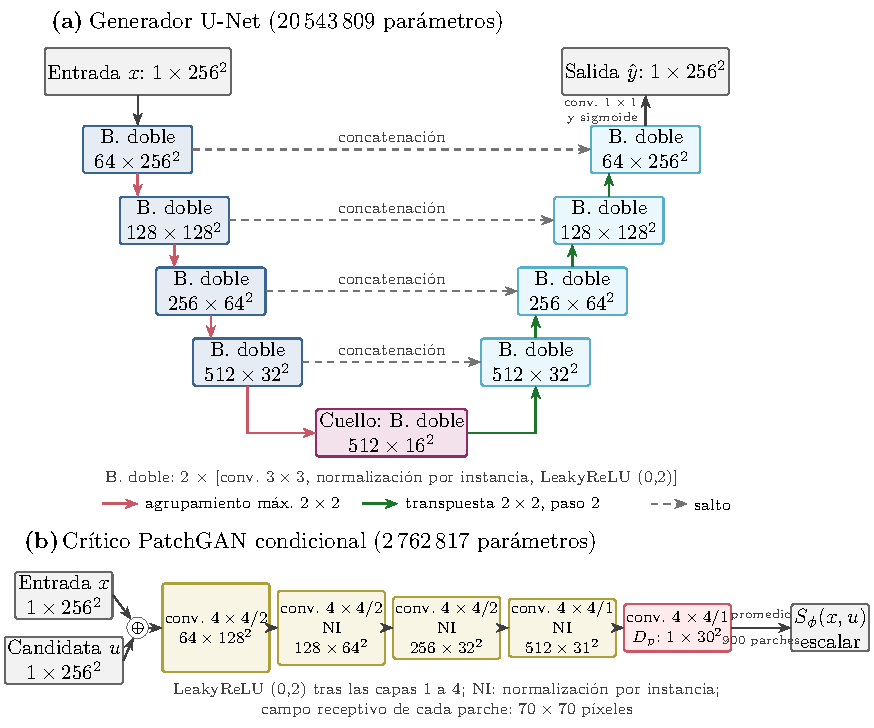
\includegraphics{fig3-5_arquitecturas.pdf}
\caption[Arquitectura del generador U-Net y del crítico PatchGAN]{Arquitectura de las redes del OE2. (a) Generador U-Net de cinco niveles: los bloques indican el número de canales y la resolución de cada nivel; las flechas horizontales discontinuas representan las conexiones de salto por concatenación. (b) Crítico PatchGAN condicional: recibe la entrada de baja estadística concatenada con la imagen candidata y produce un mapa de $30\times30$ puntuaciones, cada una con un campo receptivo de 70 píxeles, que se promedian en una puntuación escalar por muestra. Fuente: elaboración propia a partir de la implementación~v1 del repositorio de referencia.}
\label{fig:arquitecturas}
\end{figure}

\begin{table}[htbp]
\centering
\caption[Etapas del generador y capas del crítico]{Etapas del generador U-Net y capas del crítico PatchGAN de la implementación~v1. B.~doble: dos convoluciones de $3\times3$, cada una con normalización por instancia y LeakyReLU (0,2); NI: normalización por instancia; LReLU: LeakyReLU (0,2); Conv.~$4\times4$/$k$: convolución de $4\times4$ con paso $k$; Agrup.: agrupamiento máximo; Transp.: convolución transpuesta. Fuente: elaboración propia a partir de la implementación~v1 del repositorio de referencia.}
\label{tab:arquitecturas}
\small
\begin{tabular}{@{}llrrr@{}}
\toprule
Etapa & Operación & Canales & Resolución & Parámetros \\
\midrule
\multicolumn{5}{@{}l}{\emph{Generador U-Net}} \\
Codificador 1 & B.~doble & $1\to64$ & 256 & 37\,568 \\
Codificador 2 & Agrup.\ y B.~doble & $64\to128$ & 128 & 221\,440 \\
Codificador 3 & Agrup.\ y B.~doble & $128\to256$ & 64 & 885\,248 \\
Codificador 4 & Agrup.\ y B.~doble & $256\to512$ & 32 & 3\,539\,968 \\
Cuello & Agrup.\ y B.~doble & $512\to512$ & 16 & 4\,719\,616 \\
Decodificador 4 & Transp., salto y B.~doble & $512\to512$ & 32 & 8\,128\,000 \\
Decodificador 3 & Transp., salto y B.~doble & $512\to256$ & 64 & 2\,294\,528 \\
Decodificador 2 & Transp., salto y B.~doble & $256\to128$ & 128 & 573\,824 \\
Decodificador 1 & Transp., salto y B.~doble & $128\to64$ & 256 & 143\,552 \\
Salida & Conv.~$1\times1$ y sigmoide & $64\to1$ & 256 & 65 \\
\midrule
\multicolumn{4}{@{}l}{Total del generador} & 20\,543\,809 \\
\midrule
\multicolumn{5}{@{}l}{\emph{Crítico PatchGAN}} \\
Capa 1 & Conv.~$4\times4$/2, LReLU & $2\to64$ & 128 & 2\,112 \\
Capa 2 & Conv.~$4\times4$/2, NI, LReLU & $64\to128$ & 64 & 131\,072 \\
Capa 3 & Conv.~$4\times4$/2, NI, LReLU & $128\to256$ & 32 & 524\,288 \\
Capa 4 & Conv.~$4\times4$/1, NI, LReLU & $256\to512$ & 31 & 2\,097\,152 \\
Capa 5 & Conv.~$4\times4$/1 & $512\to1$ & 30 & 8\,193 \\
\midrule
\multicolumn{4}{@{}l}{Total del crítico} & 2\,762\,817 \\
\bottomrule
\end{tabular}
\end{table}

\subsection{Arquitectura del crítico PatchGAN}
\label{subsec:met-critico}

El crítico, representado en el panel~(b) de la \cref{fig:arquitecturas}, es un discriminador de parches del tipo PatchGAN \parencite{isola2017}, adaptado a la formulación de Wasserstein. Está condicionado por la entrada: recibe la imagen de baja estadística concatenada en el eje de canales con la imagen candidata, que puede ser la referencia o la salida del generador, y juzga, por tanto, si la candidata es coherente con esa entrada concreta y no solo si parece una imagen muográfica. Consta de cinco convoluciones de $4\times4$, las tres primeras con paso 2 y las dos últimas con paso unitario, con 64, 128, 256, 512 y un canal; las capas intermedias aplican normalización por instancia y todas, salvo la última, activación LeakyReLU con pendiente de 0,2. Como corresponde a un crítico de Wasserstein, la salida no pasa por una sigmoide y no está acotada. El resultado es un mapa de $P=30\times30=900$ puntuaciones $D_p$, cada una asociada a un campo receptivo de $70\times70$ píxeles, equivalente a unos $16{,}4^{\circ}$ de acimut. Ese tamaño se obtiene geométricamente de los núcleos y pasos de las capas; la elección del crítico de 70 píxeles procede de los ensayos de la etapa anterior sobre validación y no de un análisis específico con el conjunto del OE1. El crítico tiene 2\,762\,817 parámetros (\cref{tab:arquitecturas}).

\subsection{Funciones de pérdida y penalización de gradiente}
\label{subsec:met-perdidas}

El entrenamiento antagónico siguió la formulación de Wasserstein con penalización de gradiente (WGAN-GP) \parencite{arjovsky2017,gulrajani2017}, combinada con un término de reconstrucción L1 como en la traducción condicional de imágenes \parencite{mirza2014,isola2017}. Para que la puntuación que se optimiza y la que se regulariza fueran la misma, el mapa del crítico se redujo a una puntuación escalar por muestra mediante su promedio. Las pérdidas del crítico y del generador se presentan en la \cref{eq:wgan}:
\begin{subequations}\label{eq:wgan}
\begin{align}
S_\phi(x,u) &= \frac{1}{P}\sum_{p=1}^{P} D_{\phi,p}(x,u), \label{eq:wgan-score}\\
\mathcal{L}_D &= \frac{1}{B}\sum_{i=1}^{B}\Big[S_\phi\!\left(x_i,\hat y_i\right)-S_\phi\!\left(x_i,y_i\right)\Big]
 + \lambda_{\mathrm{GP}}\,\frac{1}{B}\sum_{i=1}^{B}\Big(\big\|\nabla_{\tilde y}S_\phi(x_i,\tilde y_i)\big\|_2-1\Big)^2, \label{eq:wgan-d}\\
\tilde y_i &= \alpha_i\,y_i+(1-\alpha_i)\,\hat y_i, \qquad \alpha_i\sim\mathcal{U}(0,1), \label{eq:wgan-interp}\\
\mathcal{L}_G &= -\lambda_{\mathrm{adv}}\,\frac{1}{B}\sum_{i=1}^{B}S_\phi\!\left(x_i,\hat y_i\right)+\lambda_{L1}\,\frac{1}{B\,P_y}\sum_{i=1}^{B}\big\|\hat y_i-y_i\big\|_1, \label{eq:wgan-g}
\end{align}
\end{subequations}
donde $D_{\phi,p}$ es la puntuación del parche $p$ del crítico con parámetros $\phi$, $u$ es la imagen candidata, $\hat y_i=G_\theta(x_i)$ es la salida del generador con parámetros $\theta$, $B=4$ es el tamaño del lote, $\tilde y_i$ es una interpolación aleatoria entre la referencia y la salida, $P_y=256\times256$ es el número de píxeles de la imagen, $\lambda_{\mathrm{GP}}=10$ es el peso de la penalización, $\lambda_{L1}=100$ el del término de reconstrucción y $\lambda_{\mathrm{adv}}$ el del término antagónico, igual a 1 en la cGAN. Todas las magnitudes son adimensionales, porque se calculan en el dominio normalizado de la \cref{eq:norm-v1}. La red U-Net de comparación usó el mismo generador con $\lambda_{\mathrm{adv}}=0$, es decir, solo con el término L1, sin crítico.

La revisión del código histórico encontró que la pérdida antagónica usaba el promedio del mapa, mientras que la penalización derivaba su suma. Como el gradiente de la suma es $P$ veces el del promedio, la penalización exigía en realidad que la norma del gradiente de la puntuación promedio fuera $1/P$, y no uno, lo que alteraba el objetivo de la regularización y no solo su escala. La implementación~v1 emplea la misma puntuación $S_\phi$ en la pérdida y en la penalización, como expresa la \cref{eq:wgan-d}, y doce casos analíticos con mapas de $1\times1$, $14\times14$ y $30\times30$ verificaron que la penalización vale cero cuando la norma es uno.

Los ajustes posteriores incorporaron dos términos adicionales, expresados en el espacio de cuentas mediante la inversa de la \cref{eq:norm-v1}. El primero, la pérdida regional de cuentas, penaliza la diferencia entre la cuenta media predicha y la de referencia en las regiones geométricas definidas en la sección~\ref{subsec:met-anomalias}: cielo, roca sin anomalía, borde del cono y anomalías. El segundo, la pérdida espacial de borde, penaliza el error absoluto de cuentas, píxel a píxel, en la franja del borde. Ambos se definen en la \cref{eq:perdidas-cuentas}:
\begin{subequations}\label{eq:perdidas-cuentas}
\begin{align}
\ell_R &= \left|\log\!\left(1+\overline{\hat C}_R\right)-\log\!\left(1+\overline{C^{\mathrm{ref}}}_R\right)\right|, \qquad
\mathcal{L}_{\mathrm{reg}} = \frac{1}{B}\sum_{b=1}^{B}\frac{1}{|\mathcal{F}_b|}\sum_{F\in\mathcal{F}_b}\frac{1}{|F|}\sum_{R\in F}\ell_R, \label{eq:perdida-reg}\\
\mathcal{L}_{\mathrm{borde}} &= \frac{1}{B}\sum_{b=1}^{B}\frac{\sum_{q\in E_b}\left|\hat C_b(q)-C^{\mathrm{ref}}_b(q)\right|}{\sum_{q\in E_b}C^{\mathrm{ref}}_b(q)}, \label{eq:perdida-borde}\\
\mathcal{L}_G^{\mathrm{aj}} &= \mathcal{L}_G+\lambda_{\mathrm{reg}}\,\mathcal{L}_{\mathrm{reg}}+\lambda_{\mathrm{b}}\,\mathcal{L}_{\mathrm{borde}}, \label{eq:perdida-total}
\end{align}
\end{subequations}
donde $\overline{\hat C}_R$ y $\overline{C^{\mathrm{ref}}}_R$ son las cuentas medias predichas y de referencia en la región $R$, $\hat C=T^{-1}(\hat y)$, $\mathcal{F}_b$ es el conjunto de familias de regiones con soporte de al menos veinte píxeles en la imagen $b$, $E_b$ es la región de borde de esa imagen, $\lambda_{\mathrm{reg}}$ es el peso del término regional y $\lambda_{\mathrm{b}}$ el del término de borde. Las cuatro familias pesan lo mismo y, dentro de la familia de anomalías, cada anomalía pesa lo mismo. El término regional se calculó en doble precisión mediante una identidad logarítmica que evita formar exponenciales grandes. Las máscaras intervienen solo durante el entrenamiento: el generador no las recibe y, en la inferencia, procesa únicamente la imagen de baja estadística.

El peso $\lambda_{\mathrm{reg}}=1$ se adoptó como primera hipótesis acotada, sin calibrarlo con validación. El peso del término de borde se fijó antes de su ensayo, con una regla de presupuesto de gradientes evaluada sobre doce lotes de entrenamiento, uno por geometría, con las redes iniciales congeladas y sin consultar la validación. La regla, recogida en la \cref{eq:lambda-borde}, limita la contribución del término de borde al 10\,\% de la norma del gradiente del generador en la mediana de los lotes y al 25\,\% en el peor lote:
\begin{equation}\label{eq:lambda-borde}
r_j=\frac{\left\|\nabla_\theta\mathcal{L}_{\mathrm{borde},j}\right\|_2}{\left\|\nabla_\theta\mathcal{L}^{\mathrm{C0}}_{G,j}\right\|_2}, \qquad
\lambda_{\mathrm{b}}=\frac{1}{1000}\left\lfloor 1000\,\min\!\left(1;\ \frac{0{,}10}{\operatorname{med}_j r_j};\ \frac{0{,}25}{\max_j r_j}\right)\right\rfloor,
\end{equation}
donde $r_j$ es el cociente de normas en el lote $j$ y $\mathcal{L}^{\mathrm{C0}}_{G,j}$ es la pérdida del generador sin término de borde. Con una mediana de 0,1588 y un máximo de 0,2413, la regla dio $\lambda_{\mathrm{b}}=0{,}629$. Se trata de un presupuesto de ingeniería que equilibra los términos, no de una tolerancia física.

\subsection{Entrenamiento, ajuste y selección de modelos}
\label{subsec:met-entrenamiento}

Todos los entrenamientos emplearon el optimizador Adam \parencite{kingma2015} con $\beta_1=0$ y $\beta_2=0{,}9$, valores recomendados para WGAN-GP \parencite{gulrajani2017}, tamaño de lote de 4 y cinco actualizaciones del crítico por cada actualización del generador. En cada iteración, el crítico se entrenó cinco veces con una misma salida del generador desacoplada de su grafo, y después el generador se actualizó con una salida nueva. Cada época recorrió los 1\,440 pares de entrenamiento en 360 lotes, en un orden aleatorio derivado de la semilla del ensayo y del número de época, y terminó con la evaluación completa de los 360 pares de validación. No se usaron precisión mixta ni recorte de gradientes. Para que una ejecución pudiera repetirse e interrumpirse sin alterar su resultado, se activaron los algoritmos deterministas de la biblioteca, se fijaron las semillas de todos los generadores pseudoaleatorios y cada punto de control guardó los pesos, los estados de los optimizadores y los de los generadores aleatorios.

El desarrollo del modelo se organizó como una secuencia de ensayos acotados, en la que cada uno respondió a una pregunta concreta planteada por el resultado del anterior y se diseñó antes de ejecutarse. La \cref{tab:ensayos} resume esa secuencia. El primer ensayo, un piloto al 5\,\%, entrenó desde cero la cGAN y la U-Net con idéntico generador, optimizador, semilla, normalización y presupuesto de épocas, de modo que la única diferencia fuera la componente antagónica; su pregunta era si la implementación corregida se entrenaba de forma estable y si esa componente aportaba alguna mejora. Se usó una tasa de aprendizaje de $10^{-4}$, un máximo de treinta épocas y una parada temprana después de ocho validaciones sin una mejora del SSIM de al menos 0,001; el punto de control seleccionado fue el de mayor SSIM medio en validación. Antes del piloto, una etapa técnica de dos épocas con ocho pares verificó en la GPU que el entrenamiento se reanudara tras una interrupción deliberada sin duplicar épocas y que produjera pérdidas, gradientes y métricas finitas; no se exigió en ella ninguna mejora de calidad.

\begin{table}[htbp]
\centering
\caption[Secuencia de ensayos de desarrollo del OE2]{Secuencia de ensayos de desarrollo del OE2. Todos emplearon $f=0{,}05$ y se decidieron con la partición de validación. Las continuaciones partieron de los puntos de control de la época~5 del piloto, con optimizadores nuevos, tasa de aprendizaje de $10^{-5}$ y cinco épocas adicionales. Fuente: elaboración propia a partir de los diseños y configuraciones del repositorio de referencia.}
\label{tab:ensayos}
\small
\begin{tabularx}{\linewidth}{@{}>{\raggedright\arraybackslash}p{2.3cm}>{\raggedright\arraybackslash}X>{\raggedright\arraybackslash}p{3.6cm}>{\raggedright\arraybackslash}p{2.3cm}@{}}
\toprule
Ensayo & Pregunta y variantes & Punto de partida y semillas & Criterio \\
\midrule
Piloto & ¿Se entrena la implementación corregida y aporta la componente antagónica? U-Net con L1 frente a cGAN & Desde cero; 2026100301 & Decisión descriptiva del protocolo \\
Ajuste de la U-Net & ¿Reduce el término regional el sesgo de cuentas? A: L1; B: L1 $+\ \mathcal{L}_{\mathrm{reg}}$ & U-Net del piloto; 2026100302 & Ocho controles \\
Continuación de la cGAN & Ídem en la cGAN. C0: sin $\mathcal{L}_{\mathrm{reg}}$; C1: con $\mathcal{L}_{\mathrm{reg}}$ & cGAN del piloto; 2026100303 & Ocho controles \\
Repetición R1--R3 & ¿Se mantiene la ventaja de C1 al cambiar la semilla? & cGAN del piloto; 2026100401 a 2026100403 & Ocho controles en las tres parejas \\
Ensayo de borde E1 & ¿Reduce el término espacial el error de borde sin perder lo demás? C0: con $\mathcal{L}_{\mathrm{reg}}$; C1: C0 $+\ 0{,}629\,\mathcal{L}_{\mathrm{borde}}$ & cGAN del piloto; 2026100411 a 2026100413 & Nueve controles en las tres parejas \\
\bottomrule
\end{tabularx}
\end{table}

Los ensayos siguientes ajustaron los modelos del piloto mediante continuaciones: partieron de sus pesos de la época~5, con optimizadores nuevos, una tasa de aprendizaje de $10^{-5}$ y exactamente cinco épocas adicionales, sin parada temprana, conservando siempre la quinta. Cada ensayo comparó dos variantes que solo diferían en un término de la pérdida, con la misma semilla y el mismo orden de muestras, de modo que la diferencia entre ellas pudiera atribuirse a ese término. El ajuste de la U-Net y la continuación de la cGAN añadieron la pérdida regional de la \cref{eq:perdida-reg}; la repetición R1--R3 repitió la segunda con tres semillas nuevas, para comprobar si su resultado dependía de la semilla, y el ensayo de borde E1 tomó como control la variante con pérdida regional y le añadió la pérdida espacial de la \cref{eq:perdida-borde}. Las repeticiones miden la estabilidad condicionada a un mismo punto de partida y no la variabilidad de entrenamientos independientes desde cero.

La decisión de cada ensayo se tomó con reglas fijadas en su diseño. En el ajuste, la continuación y la repetición, la variante con el término nuevo debía cumplir, frente a su control y sin redondeo, ocho controles: un indicador regional $Q$ estrictamente menor, ningún $Q$ por geometría mayor, errores de cielo y de borde no mayores, el mismo soporte de contraste, un error de contraste no mayor y un SSIM y un PSNR no menores. El ensayo de borde añadió un noveno control, que exigía un error espacial de borde estrictamente menor. Si se cumplían todos, el resultado se clasificaba como mejora concordante descriptiva; si $Q$ se reducía pero fallaba algún otro control, como compromiso; y, en otro caso, como ausencia de mejora del indicador principal. En la repetición y en el ensayo de borde, la concordancia exigía que las tres parejas cumplieran todos los controles. Ningún resultado de estos ensayos otorgaba aceptación física.

Durante la continuación de la cGAN se detectó que, en la GPU, un entrenamiento reanudado desde un punto de control no reproducía bit a bit al continuo a partir de la segunda época, aunque sí en procesador. El diagnóstico localizó la primera diferencia en los gradientes del crítico y mostró que los gradientes de la pérdida de Wasserstein y de la penalización eran exactos por separado, mientras que su suma dentro de una misma retropropagación difería en el orden de $4\times10^{-7}$. La corrección, adoptada en todas las continuaciones posteriores y descrita en el algoritmo~\ref{alg:critico}, calcula ambos gradientes por separado, los suma y aplica un único paso del optimizador, sin modificar la pérdida ni introducir tolerancias. Con ella, la reanudación reprodujo exactamente los pesos, los estados de los optimizadores y de los generadores aleatorios, los registros y las predicciones. Como el cambio de controlador de la GPU entre el diagnóstico y la aceptación no permitió aislar su efecto causal, la conclusión se limita al entorno y a la batería de pruebas empleados. El piloto se había entrenado antes de esta corrección, con la retropropagación conjunta.

\begin{algorithm}[htbp]
\caption{Iteración de entrenamiento de la cGAN con gradientes del crítico separados}
\label{alg:critico}
\begin{algorithmic}[1]
\Require lote $\{(x_i,y_i)\}_{i=1}^{B}$; generador $G_\theta$; crítico $D_\phi$; pesos $\lambda_{\mathrm{GP}}$, $\lambda_{\mathrm{adv}}$, $\lambda_{L1}$, $\lambda_{\mathrm{reg}}$, $\lambda_{\mathrm{b}}$; máscaras regionales del lote; número de pasos del crítico $n_D=5$
\Ensure parámetros actualizados $\theta$ y $\phi$
\State $\hat y_i \gets G_\theta(x_i)$ sin propagar gradientes hacia $\theta$ \Comment{salida reutilizada por el crítico}
\For{$n \gets 1$ \textbf{hasta} $n_D$}
  \State extraer $\alpha_i\sim\mathcal{U}(0,1)$ y formar $\tilde y_i$ (\cref{eq:wgan-interp})
  \State $L_W \gets \frac{1}{B}\sum_i\left[S_\phi(x_i,\hat y_i)-S_\phi(x_i,y_i)\right]$; \ $L_P \gets \lambda_{\mathrm{GP}}\,\frac{1}{B}\sum_i\left(\|\nabla_{\tilde y}S_\phi(x_i,\tilde y_i)\|_2-1\right)^2$
  \State $g_W \gets \nabla_\phi L_W$; \ después $g_P \gets \nabla_\phi L_P$ \Comment{dos retropropagaciones separadas}
  \If{alguna pérdida o gradiente no es finito} detener el entrenamiento \EndIf
  \State asignar $g_W+g_P$ como gradiente de $\phi$ y aplicar un paso de Adam
\EndFor
\State congelar $\phi$; \ $\hat y_i \gets G_\theta(x_i)$; \ $\hat C_i \gets T^{-1}(\hat y_i)$
\State calcular $\mathcal{L}_G^{\mathrm{aj}}$ con las \cref{eq:wgan-g,eq:perdida-total} y aplicar un paso de Adam sobre $\theta$
\end{algorithmic}
\end{algorithm}

Cada continuación en GPU fue precedida por una etapa técnica de aceptación, en la que una ejecución continua y otra interrumpida y reanudada debían producir resultados idénticos, y por pruebas en procesador de las pérdidas, del orden de los gradientes y de la conservación de los puntos de control. Los pesos de todas las ejecuciones quedaron identificados por su huella SHA-256 y los ocho que intervinieron en la evaluación final se fijaron en su contrato antes de la inferencia (sección~\ref{subsec:met-protocolo}).

\subsection{Métodos de referencia y estudios de ablación}
\label{subsec:met-comparadores}

Se emplearon dos comparadores. El primero es la entrada sin red, escalada a cuentas equivalentes mediante $C^{\mathrm{low}}/f$ y normalizada con la \cref{eq:norm-xy}; es el resultado que se obtendría sin procesamiento alguno y, por construcción, conserva en esperanza las cuentas de la referencia (\cref{eq:pares-media}), aunque con todo su ruido. El segundo es la U-Net entrenada solo con el término L1, que comparte con la cGAN el generador, la normalización, la semilla, el optimizador y el presupuesto de épocas, y permite atribuir al término antagónico la diferencia entre ambas. En la etapa anterior del proyecto se había empleado también un filtro clásico; como no se reimplementó con la normalización~v1 ni sobre el conjunto del OE1, no formó parte de las comparaciones de este trabajo. Los ensayos de ajuste funcionaron como estudios de ablación de un solo factor: en cada pareja, las dos variantes compartieron el punto de partida, la semilla, el orden de muestras y todos los hiperparámetros, y solo difirieron en la presencia del término regional o del término de borde.

% =============================================================================
\section{Protocolo de evaluación y estimación de la reducción de adquisición}
\label{sec:met-evaluacion}

\subsection{Diseño de la evaluación y criterios de aceptación}
\label{subsec:met-protocolo}

Los ensayos de desarrollo descritos en la sección~\ref{subsec:met-entrenamiento} se decidieron exclusivamente con la partición de validación. Una vez concluidos, la evaluación de los modelos sobre las particiones reservadas se fijó en un protocolo escrito, denominado EF-01, registrado el 4 de octubre de 2026 antes de calcular cualquier métrica de desempeño sobre esas particiones. El protocolo formuló tres preguntas: cuánto recupera la cGAN respecto de la entrada de baja estadística, cómo se compara con la U-Net entrenada con pérdida L1 y qué efecto conservan, fuera de validación, los ajustes de conservación regional y de borde. Su alcance se limitó a la fracción $f=0{,}05$, la única con modelos entrenados, y a la referencia idealizada de alta estadística del OE1; la salida evaluada es una imagen de cuentas equivalentes y no una estimación de densidad.

Se compararon nueve métodos sobre exactamente los mismos pares: la entrada sin red, escalada a cuentas equivalentes mediante $C^{\mathrm{low}}/f$, y ocho redes congeladas, cuyos pesos quedaron identificados por su huella SHA-256 en un contrato ejecutable antes de la inferencia. La \cref{tab:metodos-ef01} presenta esos métodos y su papel en la comparación. Las seis continuaciones del ensayo de borde se incluyeron completas, como análisis secundario, y no como una búsqueda de la mejor semilla; las tres parejas comparten la inicialización de la cGAN original y, por lo tanto, no estiman la variabilidad de entrenamientos independientes desde cero. El protocolo prohibió cambiar de época o de modelo según los resultados reservados y promover automáticamente el mejor valor de una tabla.

\begin{table}[htbp]
\centering
\caption[Métodos comparados en la evaluación final]{Métodos comparados en la evaluación final EF-01 con fracción $f=0{,}05$. Todas las redes se congelaron antes de la inferencia sobre las particiones reservadas. Fuente: elaboración propia a partir del protocolo EF-01 del repositorio de referencia.}
\label{tab:metodos-ef01}
\small
\begin{tabularx}{\linewidth}{@{}>{\raggedright\arraybackslash}p{3.0cm}>{\raggedright\arraybackslash}X>{\raggedright\arraybackslash}p{3.4cm}@{}}
\toprule
Método & Origen & Papel \\
\midrule
Entrada sin red & Conteos de baja estadística escalados por $1/f$ & Comparador sin procesamiento \\
U-Net original & Piloto; generador entrenado solo con pérdida L1; época 5, elegida en validación & Red de referencia \\
cGAN original & Piloto; cWGAN-GP con término L1; época 5, elegida en validación & Modelo principal \\
B1, B2, B3 -- C0 & Cinco épocas adicionales desde la cGAN original con pérdida regional de cuentas; quinta época & Análisis secundario \\
B1, B2, B3 -- C1 & Igual que C0, con el término espacial de borde añadido; quinta época & Análisis secundario \\
\bottomrule
\end{tabularx}
\end{table}

Las particiones de prueba y de generalización se evaluaron por separado. La prueba comprende tres geometrías, dieciocho vistas y 360 imágenes de entrada; la generalización, la geometría geo-gen-01, con seis vistas y 120 imágenes. Las ocho redes produjeron 3\,840 predicciones, que se compararon con las 480 entradas sin red; ninguna de ellas es una simulación nueva, pues todas proceden de los pares del OE1 con fracción 0,05.

Se fijaron de antemano seis comparaciones por partición, doce en total: la cGAN original frente a la entrada, la U-Net frente a la entrada, la cGAN original frente a la U-Net y, dentro de cada pareja B1, B2 y B3, la variante C1 frente a C0. Para cada comparación, geometría y métrica se calculó la diferencia entre el candidato y el comparador, y se registró si el candidato no empeoraba. La clasificación de la comparación sigue la \cref{eq:clasificacion}:
\begin{subequations}\label{eq:clasificacion}
\begin{align}
\delta_{g,m} &= M_{g,m}^{\mathrm{cand}} - M_{g,m}^{\mathrm{comp}}, \qquad
\nu_{g,m} = \begin{cases} 1 & \text{si } \sigma_m\,\delta_{g,m}\ge 0,\\ 0 & \text{en otro caso,}\end{cases} \label{eq:clasificacion-delta}\\
\text{clase} &= \begin{cases}
\text{sin deterioro en las métricas listadas} & \text{si } \nu_{g,m}=1 \ \ \forall\, g,m,\\
\text{compromiso o deterioro} & \text{si } \exists\, g,m:\ \nu_{g,m}=0,
\end{cases} \label{eq:clasificacion-clase}
\end{align}
\end{subequations}
donde $M_{g,m}$ es el valor de la métrica $m$ en la geometría $g$, promediado sobre sus imágenes, y $\sigma_m=+1$ para las métricas en las que un valor mayor es mejor (SSIM y PSNR) y $\sigma_m=-1$ para las de error (el indicador regional, los errores de cielo y de borde y el error de contraste), definidas en las secciones~\ref{subsec:met-calidad} y~\ref{subsec:met-anomalias}. Si alguna métrica no podía calcularse, la comparación se clasificaba como incompleta. La clasificación es descriptiva: la ausencia de deterioro no implica equivalencia ni superioridad estadística.

El plan de trabajo formuló el OE2 en términos de imágenes de calidad comparable a las de alta estadística. Sin embargo, ni el plan ni los protocolos previos fijaron un margen de equivalencia física justificado para las métricas de imagen ni para la conservación de cuentas, y el protocolo EF-01 excluyó expresamente la posibilidad de fijar ese umbral después de conocer los resultados. En consecuencia, la evaluación cuantifica concordancias y limitaciones, y una mejora frente a la entrada o frente a la U-Net no se interpreta, por sí sola, como equivalencia con la referencia.

Antes de iniciar la inferencia se registró una declaración de procedencia de las particiones reservadas. Los ocho modelos no se entrenaron, validaron ni seleccionaron con datos de prueba o de generalización: sus contratos de datos solo admitían archivos de entrenamiento y validación, y el lector de datos rechazaba las demás particiones (sección~\ref{subsec:met-particiones}). No obstante, las mismas cuatro escenas se habían simulado y evaluado en septiembre de 2026 con la versión inicial del conjunto y con modelos de la misma arquitectura, y esos resultados fueron conocidos por los autores y por la dirección. Como no puede descartarse que ese conocimiento influyera en decisiones posteriores, la evaluación EF-01 se presenta como una \emph{evaluación descriptiva sobre datos potencialmente expuestos} y no como una confirmación independiente. Este rótulo se conserva en todos los resultados del capítulo~\ref{chap:resultados}.

Conviene distinguir, por último, tres clases de decisiones. Los compromisos del plan de trabajo fijaron la arquitectura condicional, las particiones y las métricas generales. Las decisiones experimentales de la secuencia de ensayos se tomaron con validación y se describen en la sección~\ref{subsec:met-entrenamiento}. Los análisis posteriores a la apertura de las reservas, que son la corrección numérica de la selección de controles de contraste (sección~\ref{subsec:met-anomalias}) y las curvas descriptivas de exposición (sección~\ref{subsec:met-factor}), se identifican como tales y no modifican los pesos, las predicciones, las particiones ni los criterios del protocolo.

\subsection{Métricas de calidad global de imagen}
\label{subsec:met-calidad}

La calidad global se midió con el índice de similitud estructural (SSIM) y con la relación señal a ruido de pico (PSNR), calculados por imagen en el dominio normalizado de la \cref{eq:norm-v1}, en el que la referencia es $y=T(C^{\mathrm{ref}})$, la entrada sin red es $T(C^{\mathrm{low}}/f)$ y cada red entrega directamente su predicción $\hat y$, todas con rango de intensidad unitario. Ambas métricas se presentan en la \cref{eq:ssim-psnr}:
\begin{subequations}\label{eq:ssim-psnr}
\begin{align}
\mathrm{SSIM}(\hat y, y) &= \frac{1}{|W|}\sum_{w\in W}\frac{\left(2\mu_{\hat y,w}\mu_{y,w}+c_1\right)\left(2\sigma_{\hat y y,w}+c_2\right)}{\left(\mu_{\hat y,w}^{2}+\mu_{y,w}^{2}+c_1\right)\left(\sigma_{\hat y,w}^{2}+\sigma_{y,w}^{2}+c_2\right)}, \qquad c_i=(K_iL)^2, \label{eq:ssim}\\
\mathrm{PSNR}(\hat y, y) &= 10\log_{10}\frac{L^{2}}{\frac{1}{P}\sum_{q=1}^{P}\left(\hat y(q)-y(q)\right)^{2}}, \label{eq:psnr}
\end{align}
\end{subequations}
donde $W$ es el conjunto de ventanas cuadradas de $7\times7$ píxeles con pesos uniformes, $\mu$, $\sigma^2$ y $\sigma_{\hat y y}$ son la media, la varianza y la covarianza locales en cada ventana, $K_1=0{,}01$, $K_2=0{,}03$, $L=1$ es el rango de intensidad y $P=256\times256$ es el número de píxeles \parencite{wang2004}. El PSNR se expresa en decibelios; el SSIM es adimensional y vale uno para imágenes idénticas. Los parámetros se fijaron explícitamente en el código de evaluación para que no dependieran de los valores predeterminados de la biblioteca. Una predicción idéntica a la referencia tendría PSNR infinito; el protocolo previó registrarla como tal, sin confundirla con un valor nulo ni eliminarla, aunque no se presentó ningún caso.

Ambas métricas se resumieron primero por geometría, como media de sus 120 imágenes, y después como media con igual peso de las geometrías de la misma partición. El SSIM y el PSNR miden la semejanza visual y el error cuadrático en la escala logarítmica normalizada, y por ello son sensibles a la reducción del ruido de conteo. No miden, en cambio, si se conservan las cuentas de una región ni el contraste de una anomalía: una imagen suavizada puede obtener valores altos aunque desplace sistemáticamente las cuentas \parencite{hore2010}. Por esa razón se complementaron con los indicadores regionales de la sección siguiente.

\subsection{Regiones de interés y preservación de anomalías}
\label{subsec:met-anomalias}

La conservación física se evaluó en el espacio de cuentas. Cada predicción se transformó de vuelta a cuentas equivalentes con la inversa de la normalización, $\hat C=\exp\!\left(s\hat y/(1-\hat y)\right)-1$, sin recortes ni pseudocuentas, y la entrada sin red se representó por $C^{\mathrm{low}}/f$. Las regiones se derivaron de la geometría de cada escenario y no de las imágenes: para cada píxel se trazó un rayo recto desde la posición nominal del detector, a 1\,000~m del eje del cono y a 1,5~m de altura, hasta una longitud máxima de 3\,000~m, y se calculó su intersección con el cono y con las primitivas de las anomalías. Con esos rayos se definieron cuatro familias de regiones. El \emph{cielo} reúne los rayos que no cortan el cono, erosionados dos píxeles; la \emph{roca sin anomalía}, el interior del cono erosionado dos píxeles y sin las proyecciones de las anomalías, dilatadas otros dos; el \emph{borde}, la franja comprendida entre la dilatación y la erosión de dos píxeles de la silueta del cono, y cada \emph{anomalía}, los rayos que recorren al menos 20~m dentro de ella, erosionados un píxel. El umbral de 20~m es geométrico y no representa una resolución física certificada. Las regiones con menos de veinte píxeles o con cuentas de referencia nulas se registraron como no estimables, igual para todos los métodos, y no se seleccionó ninguna región según el error observado.

Para una región $R$ y una realización $k$ se calcularon el sesgo firmado y el error espacial normalizado de la \cref{eq:regiones}:
\begin{subequations}\label{eq:regiones}
\begin{align}
b_{R,k} &= \frac{\sum_{q\in R}\left(\hat C_k(q)-C^{\mathrm{ref}}(q)\right)}{\sum_{q\in R}C^{\mathrm{ref}}(q)}, \qquad
a_{R,k} = \frac{\sum_{q\in R}\left|\hat C_k(q)-C^{\mathrm{ref}}(q)\right|}{\sum_{q\in R}C^{\mathrm{ref}}(q)}, \label{eq:regiones-ba}\\
Q &= \frac{1}{2}\left(\frac{1}{V}\sum_{v=1}^{V}\left|\bar b_{\mathrm{roca},v}\right| + \frac{1}{V}\sum_{v=1}^{V}\frac{1}{|\mathcal{A}_v|}\sum_{R\in\mathcal{A}_v}\left|\bar b_{R,v}\right|\right), \label{eq:regiones-q}
\end{align}
\end{subequations}
donde $\bar b_{R,v}$ es el sesgo medio de las veinte realizaciones de la vista $v$, $V=6$ es el número de vistas de la geometría y $\mathcal{A}_v$ es el conjunto de regiones de anomalía estimables de la vista $v$. Ambas magnitudes son adimensionales y se expresan en porcentaje de las cuentas de referencia de la región. El indicador regional $Q$ promedia con igual peso el sesgo absoluto de la roca sin anomalía y el de las anomalías, estas últimas promediadas primero dentro de cada vista; resume, por tanto, el desplazamiento sistemático de las cuentas en las regiones físicamente relevantes. No representa un error de densidad ni un porcentaje de error de toda la imagen. Se exigió soporte completo: si una geometría carecía de anomalías o de regiones estimables, $Q$ se informaría como no aplicable, sin sustituirlo por cero. Los errores de cielo y de borde se obtuvieron como la media, sobre las seis vistas, del error espacial $a_{R,k}$ promediado sobre las realizaciones. El error de borde mide la fidelidad píxel a píxel en la transición entre roca y cielo, donde el gradiente de cuentas es máximo.

El contraste de una anomalía se midió frente a controles de roca geométricamente comparables, porque no se dispone de la misma geometría sin anomalía como contrafactual. Para cada píxel del núcleo de una anomalía, excluidos los rayos que atraviesan otra anomalía, se eligieron cinco píxeles de roca sin anomalía de la misma fila de elevación cuya longitud de recorrido dentro del cono difiriera en no más del 5\,\%, escogidos por cercanía de esa longitud. Con esos controles, el contraste y su error se definieron en la \cref{eq:contraste}:
\begin{equation}\label{eq:contraste}
\mathcal{C}_k=\frac{\overline{C}_{\mathrm{obj},k}}{\overline{C}_{\mathrm{ctrl},k}}-1, \qquad
e_{\mathcal{C}}=\frac{1}{K_{\mathrm{v}}}\sum_{k=1}^{K_{\mathrm{v}}}\left|\mathcal{C}_k-\mathcal{C}^{\mathrm{ref}}\right|,
\end{equation}
donde $\overline{C}_{\mathrm{obj},k}$ y $\overline{C}_{\mathrm{ctrl},k}$ son las cuentas medias de los píxeles objetivo y de sus controles en la realización $k$, $\mathcal{C}^{\mathrm{ref}}$ es el mismo contraste calculado sobre la referencia y $K_{\mathrm{v}}$ es el número de realizaciones con control no nulo. El contraste es adimensional y corresponde a la intensidad de conteo, no a la opacidad. Una combinación de anomalía y vista se consideró estimable si reunía al menos veinte píxeles emparejados y una cobertura mínima del 80\,\% de su núcleo; el error medio de cada partición se calculó solo sobre el soporte común, formado por las combinaciones con veinte realizaciones válidas en todos los métodos, cuyo número se informa junto a cada resultado.

Después de abrir las reservas, una reevaluación independiente en otro sistema operativo difirió de la original en cuatro contrastes. El análisis mostró que algunos candidatos a control tenían longitudes prácticamente iguales y que ordenarlos sin tolerancia podía intercambiar el quinto donante por redondeos de la última cifra. La dirección del proyecto estableció entonces la corrección numérica C2, que se resume en el algoritmo~\ref{alg:controles}: se conservan la elegibilidad y los cinco controles por píxel, pero los candidatos cuya diferencia de longitud dista menos de $10^{-8}$~m de la del candidato más cercano se agrupan y se desempatan por columna ascendente, sin encadenar empates. La tolerancia se fijó antes de leer las métricas corregidas, se aplicó por igual a todos los escenarios, anomalías y métodos, y resuelve diferencias próximas a la precisión numérica sin representar una resolución espacial física. Los índices de los controles resultantes se registraron con las huellas de sus máscaras, de modo que una reproducción posterior los reutiliza en lugar de seleccionarlos de nuevo.

\begin{algorithm}[htbp]
\caption{Selección de controles de contraste con tolerancia de empate (corrección C2)}
\label{alg:controles}
\begin{algorithmic}[1]
\Require núcleo de anomalía $\mathcal{T}$; máscara de roca sin anomalía $\mathcal{R}$; longitud de recorrido en el cono $\ell(q)$ de cada píxel; tolerancia relativa $\eta=0{,}05$; número de controles $K_c=5$; tolerancia de empate $\tau=10^{-8}$~m
\Ensure índices de los controles de cada píxel emparejado y su registro con huellas
\For{cada píxel $q\in\mathcal{T}$}
  \State $\mathcal{K}\gets\{r\in\mathcal{R}:\ \text{fila}(r)=\text{fila}(q),\ |\ell(r)-\ell(q)|\le\eta\,\ell(q)\}$
  \State $d(r)\gets|\ell(r)-\ell(q)|$ para cada $r\in\mathcal{K}$; $\mathcal{D}\gets\emptyset$
  \For{cada ancla $d^{*}=\min_{r\in\mathcal{K}} d(r)$, en orden creciente, mientras $|\mathcal{D}|<K_c$ y $\mathcal{K}\neq\emptyset$}
    \State $\mathcal{G}\gets\{r\in\mathcal{K}:\ d(r)-d^{*}\le\tau\}$, sin encadenar empates, ordenado por columna ascendente
    \State añadir a $\mathcal{D}$ los primeros elementos de $\mathcal{G}$ hasta completar $K_c$; \ $\mathcal{K}\gets\mathcal{K}\setminus\mathcal{G}$
  \EndFor
  \If{$|\mathcal{D}|=K_c$} registrar $q$ como emparejado con los controles $\mathcal{D}$ \EndIf
\EndFor
\If{hay al menos 20 píxeles emparejados \textbf{y} cubren al menos el 80\,\% de $\mathcal{T}$}
  \State marcar la combinación como estimable y guardar sus índices y la huella de las máscaras
\Else
  \State marcar la combinación como de geometría insuficiente
\EndIf
\end{algorithmic}
\end{algorithm}

La corrección se verificó con cuatro pruebas específicas, que cubren el orden de empates próximos, la separación entre distancia y elegibilidad, la reproducción con rechazo de índices alterados y el rechazo de soportes modificados, y con 162 comprobaciones de sensibilidad sobre los 54 conjuntos de controles: tolerancias de $10^{-9}$ y $10^{-7}$~m y una perturbación determinista de $\pm10^{-10}$~m en las longitudes, que conservaron exactamente los índices de C2. Estas pruebas acotan la sensibilidad dentro del catálogo, pero no constituyen una garantía universal. La corrección no altera el SSIM, el PSNR ni los indicadores regionales, que no dependen de los controles.

\subsection{Análisis estadístico y tratamiento de la dependencia}
\label{subsec:met-estadistica}

La unidad de inferencia sobre escenarios es la geometría (sección~\ref{subsec:met-enfoque}). Las veinte realizaciones de una vista comparten la referencia y los muones de las entradas son subconjuntos de ella, de modo que no constituyen observaciones independientes; las seis vistas de una geometría comparten, a su vez, el mismo edificio. Con tres geometrías de prueba y una de generalización, el número de unidades independientes es insuficiente para estimar intervalos de confianza o pruebas de hipótesis con interpretación poblacional, y tratarlas como 360 o 120 observaciones independientes habría subestimado la incertidumbre. Por esa razón, el análisis se limitó a la descripción: se informaron las medias por geometría y sus macropromedios con igual peso, se calcularon las diferencias entre métodos para cada geometría y se registró si su signo se repetía en todas ellas. Las comparaciones entre métodos son emparejadas, porque todos se evaluaron sobre las mismas entradas y la misma referencia.

Las particiones de prueba y de generalización se analizaron por separado y nunca se agregaron. La ausencia de diferencias favorables en una comparación no se interpretó como equivalencia, y las diferencias favorables no se interpretaron como superioridad estadística. Las tablas completas por geometría, vista, realización y región se conservaron junto con los macropromedios, para que ninguna conclusión dependa únicamente de un promedio.

\subsection{Estimación del factor de reducción de adquisición}
\label{subsec:met-factor}

La relación entre fracción de conteos y tiempo de adquisición se apoya en el modelo de conteo de la sección~\ref{subsec:met-pares}. Con flujo estable y condiciones de detección iguales, la esperanza del número de muones registrados crece linealmente con la exposición, como expresa la \cref{eq:factor}:
\begin{equation}\label{eq:factor}
\mathrm{E}\!\left[N(t)\right]=\lambda\,t, \qquad
f=\frac{t_{\mathrm{bajo}}}{t_{\mathrm{ref}}}, \qquad
R=\frac{f_{\mathrm{ent}}}{f_{\mathrm{mod}}},
\end{equation}
donde $\lambda$ es la tasa de muones registrados, en muones por unidad de tiempo, $t$ es la exposición, $f$ es la fracción de conteos que conserva una adquisición corta de duración $t_{\mathrm{bajo}}$ frente a la referencia de duración $t_{\mathrm{ref}}$, y $R$ es la razón nominal entre la exposición de una entrada sin red con fracción $f_{\mathrm{ent}}$ y la de la entrada del modelo, con $f_{\mathrm{mod}}=0{,}05$. Con $f=0{,}05$, el factor nominal frente a la referencia completa es $1/f=20$. Como las entradas se construyeron por adelgazamiento de una misma referencia, este factor es una equivalencia idealizada de exposición y no una medición de tiempo de campo; la duración del entrenamiento o de la inferencia tampoco es un tiempo de adquisición.

Determinar un factor alcanzable exige especificar antes qué calidad se considera aceptable. Como ese criterio no se había fijado al cerrar la evaluación del OE2, se realizó únicamente un análisis descriptivo con los datos ya disponibles: se calcularon las mismas métricas de la entrada sin red con las fracciones 0,01, 0,05, 0,10 y 0,50 sobre las particiones reservadas, con la normalización y las regiones del protocolo EF-01, y se compararon con las ocho redes, evaluadas únicamente con $f=0{,}05$. El caso de 0,05 se conservó como control, pues debía reproducir los valores de la entrada en EF-01. Para el contraste se usó el soporte común a las cuatro fracciones y a las ocho redes, porque con la fracción 0,01 algunas realizaciones tienen controles con cero cuentas. Las líneas que unen los cuatro puntos se emplearon solo como guía visual: no se interpoló entre fracciones, no se extrapoló fuera de la rejilla y no se trató la referencia comparada consigo misma como un punto de PSNR infinito. Se distinguieron tres niveles de lectura que no deben confundirse: la reducción nominal de conteos, la equivalencia descriptiva según SSIM y PSNR, y la aceptación física según cuentas y contraste. Este análisis es posterior a la apertura de las reservas y no permite afirmar el desempeño de las redes con otras fracciones de entrada.

\subsection{Generalización, sensibilidad y análisis de fallos}
\label{subsec:met-generalizacion}

La geometría geo-gen-01 se reservó para estimar el comportamiento en un escenario no representado en las particiones de entrenamiento, validación y prueba, y se informó siempre por separado. Al tratarse de una sola geometría, sus resultados describen ese escenario y no una tasa de generalización. La sensibilidad de los resultados se examinó en dos aspectos: la estabilidad numérica de la selección de controles, descrita en la sección~\ref{subsec:met-anomalias}, y la reproducibilidad del cálculo de métricas, que se recalculó de forma independiente en otro equipo a partir de las predicciones conservadas. El análisis de fallos se apoyó en los resultados por geometría y por anomalía, incluidos los cambios de signo del contraste respecto de la referencia, sin seleccionar casos favorables o desfavorables con posterioridad. Todos estos análisis tienen carácter exploratorio, y una buena calidad global de imagen no se equiparó con la detectabilidad física de una anomalía.

% =============================================================================
\section{Entorno computacional, reproducibilidad y trazabilidad}
\label{sec:met-reproducibilidad}

\subsection{Infraestructura y dependencias de software}
\label{subsec:met-entorno}

La simulación del OE1 se ejecutó en el supercomputador SC3 de la Universidad Industrial de Santander, con una cuenta del grupo de investigación. Los ensayos previos y el piloto de seis vistas emplearon la partición \texttt{legacy}, con procesadores Intel Xeon E5645 y 24 hilos por trabajo; la campaña definitiva empleó la partición \texttt{amd}, cuyos nodos cuentan con procesadores AMD EPYC 9554 y 9534, con 64 hilos, 8~GB de memoria y un límite de 15 minutos por trabajo. Antes de la campaña se comprobó la portabilidad de la receta entre ambas particiones: un mismo bloque de $5\times10^{6}$ primarios produjo histogramas idénticos byte a byte con 24 hilos en \texttt{legacy} y con 64 hilos en \texttt{amd}. El entorno de compilación y ejecución se cargó mediante los módulos del clúster para el compilador GCC 14.2.0 y para Geant4 11.4.2, siempre a partir de un entorno limpio, porque las primeras compilaciones enlazaron por error contra la biblioteca estándar del compilador del sistema. EcoMug y la biblioteca de lectura de JSON se incluyeron en el código fuente, de modo que la aplicación puede compilarse sin conexión a internet. La \cref{tab:software} resume las versiones registradas.

Cada componente cumplió un papel preciso en el OE1. Geant4 realizó el transporte de los muones a través del edificio (sección~\ref{subsec:met-transporte}); EcoMug aportó el espectro de momento y la razón de carga por medio de las tablas del generador (sección~\ref{subsec:met-fuente}); y Python implementó el motor analítico, la construcción de las tablas, las validaciones, la publicación y la fusión de los bloques, la evaluación de la calidad, la exportación de las imágenes y la construcción de los pares, con apoyo de las bibliotecas NumPy y SciPy \parencite{harris2020}. El repositorio conserva, además, una receta de contenedor que declara una versión anterior de Geant4; esa receta no se empleó en la campaña y no se ha validado como una vía de reproducción exacta.

\begin{table}[htbp]
\centering
\caption[Versiones de software de la simulación del OE1]{Versiones de software registradas para la simulación del OE1. Fuente: elaboración propia a partir de la receta operativa y de los registros de entorno del repositorio de referencia.}
\label{tab:software}
\small
\begin{tabularx}{\linewidth}{@{}lX@{}}
\toprule
Componente & Versión registrada \\
\midrule
Geant4 & 11.4.2, multihilo; lista de física \texttt{FTFP\_BERT} \\
Compilador & GCC 14.2.0; estándar C++17 \\
EcoMug & 2.2, incluido en el código \\
Biblioteca JSON para C++ & 3.11.3, incluida en el código \\
Posproceso en el clúster & Python 3.13.13, NumPy 2.5.2, SciPy 1.18.1 \\
Construcción de los pares & NumPy 2.4.4 (versión fijada) \\
Receta de contenedor & Geant4 11.3.2 declarado; no validada ni empleada \\
\bottomrule
\end{tabularx}
\end{table}

El entrenamiento y la inferencia del OE2 no se ejecutaron en el supercomputador de la universidad, cuyas GPU estaban ocupadas y cuyo espacio de usuario estaba casi agotado durante el período de los ensayos, sino en un servicio de computación en la nube, con GPU NVIDIA L40S de 46~GB: dos en paralelo en el piloto, una en los ajustes de la U-Net y de la cGAN, tres en paralelo en la repetición y en el ensayo de borde, y una en la evaluación final. Python y PyTorch implementaron las redes, el entrenamiento, la inferencia y la evaluación; scikit-image proporcionó el SSIM y el PSNR, y NumPy y SciPy los cálculos regionales \parencite{harris2020}. El plan de trabajo preveía MATLAB entre sus recursos, pero la implementación heredada de la etapa anterior del proyecto estaba escrita en Python con PyTorch, y no se empleó MATLAB en ninguna etapa. En las continuaciones y en la evaluación final se desactivó la aritmética TF32, de modo que todas las operaciones se realizaron en coma flotante de 32 bits; la configuración del piloto no fijó esa opción de forma explícita. Las reevaluaciones independientes, la corrección del contraste y las curvas de exposición se calcularon en procesador, sin GPU. La \cref{tab:software-oe2} resume las versiones registradas.

\begin{table}[htbp]
\centering
\caption[Versiones de software del modelo y de su evaluación]{Versiones de software y equipos registrados para el entrenamiento y la evaluación del modelo (OE2) y para los análisis posteriores. Fuente: elaboración propia a partir de los registros de entorno del repositorio de referencia.}
\label{tab:software-oe2}
\small
\begin{tabularx}{\linewidth}{@{}lX@{}}
\toprule
Componente & Versión registrada \\
\midrule
Lenguaje y aprendizaje profundo & Python 3.12.3; PyTorch 2.6.0 con CUDA 11.8 y cuDNN 9.1.0 \\
Bibliotecas numéricas & NumPy 2.3.5 (2.4.4 en el piloto); SciPy 1.18.1 \\
Métricas de imagen & scikit-image 0.26.0 \\
Equipo de entrenamiento e inferencia & GPU NVIDIA L40S de 46~GB en un servicio de computación en la nube \\
Reevaluación, corrección C2 y curvas & Python 3.12.14; PyTorch 2.6.0 en procesador; NumPy 2.3.5; scikit-image 0.26.0 \\
\bottomrule
\end{tabularx}
\end{table}

\subsection{Identificación y conservación de datos y modelos}
\label{subsec:met-artefactos}

Cada producto del OE1 quedó identificado por dos elementos complementarios: la semilla que lo generó y una huella criptográfica de su contenido. La huella SHA-256 \parencite{nist2015} identifica de forma unívoca el contenido de un archivo, pues cualquier cambio de un solo byte la altera; por ello se registró en cada etapa: la de la receta y el manifiesto antes del envío, la de los archivos de cada bloque en su recibo de publicación, la de los histogramas fusionados y sus metadatos en el inventario de la fusión, la de cada imagen exportada en el inventario de la exportación y la de cada archivo de pares, junto con las huellas de contenido de sus arreglos, en el inventario del empaquetado. Una fecha, en cambio, solo data el momento en que se fijó un producto: una reconstrucción podría conservarla y producir, aun así, archivos distintos. Por esa razón, la identidad del conjunto se estableció con las huellas y no con fechas. La \cref{tab:semillas} reúne las semillas de la cadena de simulación.

\begin{table}[htbp]
\centering
\caption[Semillas de la cadena de simulación del OE1]{Semillas registradas en la cadena de simulación del OE1. Fuente: elaboración propia a partir del repositorio de referencia.}
\label{tab:semillas}
\small
\begin{tabularx}{\linewidth}{@{}>{\raggedright\arraybackslash}p{6.2cm}>{\raggedright\arraybackslash}X@{}}
\toprule
Uso & Semilla o derivación \\
\midrule
Catálogo de escenarios & 20260805, con un generador independiente derivado por geometría \\
Muestra de EcoMug & 20260805 \\
Validación del muestreador y pruebas físicas del motor analítico & 20260805; la prueba de exactitud de tablas usa 123 \\
Diagnóstico de geo-train-06 y control geométrico & 20260929; la simulación de control T4 usa 2026092900 \\
Ensayo piloto de la corrección & 2026092801, 2026092802 y 2026092803 \\
Campaña definitiva & \cref{eq:semilla-campana}; 1\,026 semillas únicas, distintas de las del piloto de seis vistas \\
Adelgazamiento binomial & semilla maestra 20260805, con derivación por geometría, vista, fracción y realización \\
\bottomrule
\end{tabularx}
\end{table}

El repositorio de referencia conserva el código, las configuraciones, la receta, el manifiesto, los registros del gestor de trabajos, los 114 histogramas fusionados con sus metadatos y las 114 imágenes exportadas, todos con sus inventarios de huellas. Los archivos de pares, que ocupan cerca de 547~MB, se distribuyeron en una copia compartida acompañada de un documento con las versiones, los commits y las huellas empleadas; los 1\,026 bloques publicados, que ocupan unos 734~MB, se conservan en el supercomputador con su inventario de huellas registrado en el repositorio.

En el OE2 se aplicó el mismo principio. Cada configuración de entrenamiento registró su semilla, la partición de entrenamiento, la de selección, la prohibición de acceder a las particiones reservadas, la escala de normalización y la huella del punto de partida, y cada punto de control quedó identificado por su huella SHA-256; las semillas de los ensayos se indican en la \cref{tab:ensayos}. El contrato de la evaluación final fijó las huellas de los ocho pesos, de los archivos de datos de las cuatro geometrías reservadas y del código de evaluación, y el evaluador se negó a ejecutarse si alguna no coincidía. Las 3\,840 predicciones, que forman 32 matrices de $120\times256\times256$ valores en coma flotante y ocupan 1\,006\,637\,056 bytes, se acompañaron de recibos con sus huellas. La corrección C2 guardó, además, los índices exactos de los controles de contraste con las huellas de sus máscaras. Una huella identifica el contenido, pero no data el momento en que se fijó; por ello, la anterioridad del protocolo y de la declaración de procedencia respecto de la inferencia se sustenta en el orden de los registros del repositorio y no en un sello temporal certificado. El repositorio de referencia conserva las configuraciones, los registros, las métricas y las huellas; los pesos y las predicciones, por su tamaño, se distribuyeron en copias compartidas cuyo acceso público se verificó descargando archivos y contrastando sus huellas.

\subsection{Verificación del software y procedimiento de reproducción}
\label{subsec:met-reproduccion}

La integridad del conjunto se verificó con herramientas que no ejecutan simulaciones ni modifican los datos, acompañadas de pruebas automáticas con datos sintéticos que cubren, entre otros, manifiestos y máscaras alterados, semillas y ejecutables incorrectos y campañas incompletas. La reproducción se entendió en dos niveles. El primero, la reproducción desde los datos originales, repite los cálculos a partir de las entradas primarias y compara los productos resultantes con los registrados. En ese nivel se repitió la evaluación de calidad desde los histogramas fusionados, con el plan, la receta y las máscaras congelados; se comprobó que las imágenes exportadas conservaran exactamente los conteos y las coordenadas de los histogramas, y se regeneraron los 9\,120 pares desde las 114 imágenes, de forma independiente, en una segunda máquina de los estudiantes y en la revisión de la dirección, en ambos casos con NumPy 2.4.4. Como las huellas de los archivos comprimidos dependen de la biblioteca de compresión, la regeneración se contrastó con las huellas de contenido de los 342 arreglos de los pares. Por último, la copia de distribución se recuperó desde su enlace con una cuenta distinta de la propietaria y se contrastó, archivo por archivo, con los inventarios del repositorio.

Para el transporte, en cambio, no se dispuso de una segunda ejecución independiente de la campaña: la verificación se apoyó en los registros del gestor de trabajos, en los recibos de cada bloque y en la prueba de portabilidad entre particiones descrita en la sección~\ref{subsec:met-entorno}. Durante el proyecto, una reconstrucción de los pares del conjunto inicial con otra versión de la biblioteca numérica había producido realizaciones binomiales distintas, lo que llevó a fijar la versión empleada y a verificar las huellas al terminar cada construcción.

El segundo nivel, el recálculo a partir de valores almacenados, reconstruye tablas y totales desde los metadatos y registros, como la suma de los primarios transportados y registrados de la campaña o las horas de cómputo asignadas. Ese recálculo comprueba la coherencia interna de los registros, pero no constituye una reproducción, porque no vuelve a generar los datos.

En el OE2, la reproducción desde los datos originales se verificó en varios puntos. En el entrenamiento, la aceptación técnica de cada continuación exigió que una ejecución interrumpida y reanudada reprodujera exactamente a la continua (sección~\ref{subsec:met-entrenamiento}). En la inferencia de los ajustes, la repetición y el ensayo de borde, los pesos se volvieron a aplicar en procesador sobre las imágenes de validación, y las diferencias por píxel frente a las predicciones de la GPU no superaron $10^{-5}$. En la evaluación final, la revisión de la dirección recalculó, desde las 3\,840 predicciones y las 480 entradas, las métricas de todas las imágenes, que coincidieron exactamente, y las regionales, con diferencias máximas de $4{,}44\times10^{-16}$; además, volvió a inferir con los pesos originales cuatro imágenes de una geometría de prueba por cada red, con una diferencia máxima de $4{,}85\times10^{-6}$, comprobación que es una muestra y no una repetición completa de la inferencia. Una segunda evaluación completa con el registro de controles de la corrección C2 reprodujo su informe byte a byte, y en el análisis de exposición el caso de 0,05 reprodujo los valores de la entrada de la evaluación final con una tolerancia de $10^{-12}$. No se repitió, en cambio, ningún entrenamiento completo de forma independiente: la reproducibilidad del entrenamiento se apoya en la recuperación exacta y en las huellas, no en una segunda ejecución. Las tablas del capítulo~\ref{chap:resultados} se recalcularon a partir de las métricas almacenadas, lo que comprueba su coherencia con los registros pero no constituye una reproducción.

\subsection{Trazabilidad de decisiones y limitaciones metodológicas}
\label{subsec:met-decisiones}

La generación del conjunto se realizó en tres pasadas. La primera empleó el motor analítico para validar el diseño de extremo a extremo con un costo computacional mínimo. La segunda sustituyó el motor analítico por el transporte con Geant4, con el mismo catálogo y el mismo formato de datos, y dio lugar al conjunto inicial. La tercera incorporó las decisiones derivadas de su revisión técnica: la construcción corregida de las anomalías, la malla angular de intervalos iguales, la inyección junto a la roca con margen angular de 5°, el umbral de registro de 3~GeV, el número fijo de primarios por vista y los criterios de calidad registrados antes del envío. La dirección del proyecto adoptó el alcance idealizado del producto y acordó con los estudiantes, antes de la campaña, el presupuesto de $3{,}44\times10^{8}$ primarios por vista, la meta descriptiva de roca y el tratamiento de las vistas que no la alcanzaran. Se optó por una campaña nueva, en lugar de completar las vistas del piloto, para no alterar sus recibos ni la definición de la evaluación confirmatoria.

La metodología del OE1 tiene limitaciones que conviene declarar antes de presentar sus resultados. En la geometría, los escenarios son conos idealizados sin topografía circundante; no se dispuso de un control independiente para los volúmenes que sobresalen del edificio en geo-gen-01 y geo-test-03, y los casos que combinan recorte y sustracción múltiple no se ensayaron por separado. En la fuente, el modelo híbrido y su extensión fuera de la ventana son hipótesis del conjunto y no un flujo calibrado. En el transporte, solo se siguieron muones primarios, sin partículas secundarias, respuesta instrumental ni fondo experimental, y el plano de conteo es una superficie computacional que no equivale a un detector físico de 1,2~m, cuya equivalencia no se demostró. En la normalización, la exposición es una escala convencional y la referencia ideal de cielo no incluye pérdidas en el aire, desintegración, dispersión ni migración angular. En el muestreo, las veinte realizaciones de una vista comparten su referencia y la referencia conserva su propio ruido, y las máscaras de roca ignoran las anomalías. Por último, en la procedencia, la versión de EcoMug empleada en la muestra no quedó fijada a una revisión exacta y algunos insumos históricos de las primeras etapas no se conservaron. Las consecuencias observadas de estas limitaciones se analizan en el capítulo~\ref{chap:resultados}.

El desarrollo del modelo se apartó del plan de trabajo en varios aspectos que conviene declarar. Se entrenaron modelos para una sola fracción, $f=0{,}05$, en lugar de la campaña de entrenamientos con las cuatro fracciones que se había previsto; las arquitecturas se heredaron de la etapa anterior y no se volvieron a seleccionar con el conjunto del OE1; el filtro clásico de esa etapa no se incluyó en las comparaciones, y el cómputo se realizó en la nube y no en el supercomputador. La dirección del proyecto revisó el código heredado y estableció las correcciones de la implementación~v1, aprobó la secuencia de ensayos, autorizó la evaluación final, estableció la corrección numérica del contraste y dio por cerrada la parte experimental del OE2 sin pedir más entrenamientos. Ninguna de esas decisiones fijó un margen de equivalencia física, de modo que la expresión del plan sobre una calidad comparable a la de alta estadística no pudo convertirse en un criterio de aceptación.

Las limitaciones del OE1 se transmiten al modelo: las referencias son idealizadas y conservan su propio ruido, las realizaciones de una vista comparten la referencia y las imágenes no equivalen a las de un detector físico. A ellas se suman las propias del OE2. Las continuaciones comparten la inicialización y no estiman la variabilidad desde cero; las particiones reservadas contienen tres geometrías de prueba y una de generalización, ya evaluadas en una etapa anterior; el indicador regional resume sesgos de cuentas en regiones geométricas y no errores de densidad, y la normalización depende de una escala ajustada con la partición de entrenamiento. En el OE3, el factor nominal de reducción es una equivalencia idealizada derivada del adelgazamiento binomial y no un tiempo de campo medido. Las consecuencias observadas de estas limitaciones se analizan en el capítulo~\ref{chap:resultados}.

\chapter{Resultados y discusión}
\label{chap:resultados}

% Versión 4: incorpora los resultados y la discusión del OE2 y la parte sustentada del
% OE3 (muografia-documentada, rama principal 08cdc0c: revisión EF-01-C2, síntesis del
% OE2 y curvas descriptivas de exposición). Cifras generadas desde los JSON del repositorio.
% Versión 3: incorpora los resultados y la discusión del OE1 (campaña de 114 vistas).
% Cifras contrastadas con la entrega f395570 de muografia-documentada y con las
% revisiones de la dirección (c4e467f, efeee44, 58f9c12 y 4529c49).

Este capítulo presenta los resultados obtenidos con los procedimientos del capítulo~\ref{chap:metodologia} y su interpretación. Se organiza en tres secciones, una por objetivo específico: el conjunto de datos sintéticos, su calidad y su reproducibilidad (OE1); los ensayos de desarrollo del modelo y su evaluación final (OE2), y el análisis descriptivo del desempeño frente a la exposición (OE3). En cada una se mantiene la distinción de la metodología entre resultados confirmatorios, descriptivos y exploratorios, y se indica el criterio con el que se interpreta cada resultado. Los resultados de los objetivos segundo y tercero sobre las particiones reservadas tienen carácter descriptivo, porque esas escenas habían sido evaluadas en una etapa anterior del proyecto (sección~\ref{subsec:met-protocolo}).

% =============================================================================
\section{Conjunto de datos sintéticos del OE1}
\label{sec:res-oe1}

Los resultados de esta sección proceden de la campaña de 114 vistas ejecutada entre el 2 y el 3 de octubre de 2026 y de los ensayos que la precedieron. Todas las cifras se obtuvieron de los registros, inventarios y evaluaciones conservados en el repositorio de referencia, y las de la campaña se contrastaron, además, con la revisión directa de la dirección, que repitió la evaluación desde los histogramas y regeneró los pares de forma independiente. La exposición sigue el orden de la cadena: primero los ensayos previos, después la ejecución y la integridad de la campaña, luego los dos indicadores de calidad de las referencias y, por último, la discusión del producto obtenido.

\subsection{Resultados de los ensayos previos a la campaña}
\label{subsec:res-ensayos}

Las comprobaciones del generador confirmaron la normalización de la fuente. La escala $S_0$ recalculada directamente desde la parametrización de Guan difirió de la tabla en $6{,}2\times10^{-5}$ en términos relativos, y la prueba $\chi^2$ de la distribución de direcciones por filas de elevación, con 255 grados de libertad, dio valores de 290,4, 224,3 y 265,1 en tres simulaciones independientes, con valores $p$ aproximados de 0,06, 0,92 y 0,32; sumada sobre una imagen completa, la relación de la \cref{eq:fuente-t} reprodujo el conteo total con un cociente de 1,00014.

Los ensayos de la corrección geométrica mostraron que la regla B1 eliminó las advertencias de superposición en los controles ejecutados, sin evidencia de un cambio en los conteos que la estadística disponible pudiera resolver. El piloto A/B sobre geo-train-06 resultó inconcluso, como se había anticipado en su prerregistro por falta de potencia en la región de intersección. La primera etapa del segundo ensayo, con 1\,300\,000 transportes de producción incluida la repetición técnica, dio una diferencia estimada nula en la región de interés en ambas geometrías, con un intervalo diagnóstico de aproximadamente $\pm12{,}8$ cuentas por millón de primarios, y su repetición A/A fue idéntica byte a byte a la referencia; sin embargo, solo un muon de producción cruzó la región de intersección, sin llegar al detector, y los cruces sintéticos de control entraron todos desde el cuerpo denso, de modo que no se contrastó la entrada desde el conducto. El complemento dirigido cubrió esa situación: la variante corregida asignó la región compartida al cuerpo denso en los 36 pares de trayectorias, mientras que la variante original la asignó al conducto en los 18 casos dirigidos desde ese lado; tres pares cambiaron de píxel y ninguno cambió su detección. La segunda etapa, con el tamaño fijado de antemano, estimó una diferencia de $+0{,}125$ detecciones por millón de primarios con un intervalo conservador del 95\,\% de $[-0{,}229;\ +0{,}469]$ por millón, de modo que su resultado fue inconcluso: no demostró equivalencia dentro del margen ni una diferencia relevante fuera de él, y el diseño no preveía ampliar el tamaño. La auditoría independiente de sus registros superó 6\,966 controles sin fallos.

Los controles del observable fijaron la receta de producción. Con la inyección 1~m antes de la roca y el umbral de 3~GeV, la razón de conteos entre los planos de 100 y 600~m fue, por bandas de espesor másico de roca, de 1,000, 0,999, 0,994, 0,990 y 0,991, con un mínimo de $0{,}9895\pm0{,}0025$, y ese umbral conservó el 83,5\,\% del conteo en roca; entre los planos de 600 y 1\,200~m la diferencia fue nula. La misma inyección elevó la eficiencia de cielo abierto, sin umbral, al 99,97\,\% de media, con una fila mínima de 99,69\,\%; la variante intermedia fijada de antemano no había cumplido el criterio, y la inyección junto a la roca se añadió después y se evaluó con el mismo criterio. En los bordes, ninguna configuración cumplió el criterio estricto de los controles cortos: con la inyección junto a la roca y un margen de 5°, el sesgo medio desapareció ($-0{,}07$ puntos porcentuales) y la desviación máxima fue de 1,65 puntos porcentuales, de modo que ese control quedó abierto y su verificación se trasladó al criterio de bordes de la campaña. Con los datos anidados, solo entre el 3,6 y el 70,4\,\% de los registros del plano de 600~m, según la banda de espesor, cayeron dentro del panel de 1,2~m, lo que confirma que la convergencia entre planos grandes no informa sobre la equivalencia con el panel. La integración de la malla angular, con 1\,000 primarios, produjo 750 registros y superó sus controles de metadatos, histograma, registro y código de salida.

Por último, el piloto de seis vistas, con $2{,}11\times10^{8}$ primarios por vista, completó sus 36 bloques sin fallos y sus 90 regiones de borde quedaron dentro de la tolerancia de $\pm1$ punto porcentual. En la roca, la mediana fue de 121 a 127 cuentas por región y entre el 63 y el 65\,\% de las regiones alcanzó 100 cuentas. Con esas tasas, una proyección binomial a $3{,}44\times10^{8}$ primarios estimó una fracción media de regiones con al menos 100 cuentas de 89,7 a 91,1\,\% para esa geometría; la proyección no garantizaba el 90\,\% en todas las vistas, y así quedó registrado en el acuerdo previo a la campaña.

\subsection{Ejecución e integridad de la campaña}
\label{subsec:res-campana}

La campaña se ejecutó entre el 2 de octubre de 2026 a las 18:10:27 y el 3 de octubre a las 09:48:49, unas 15,6 horas de reloj. La \cref{tab:ejecucion} resume su ejecución. Los 1\,026 bloques del manifiesto terminaron y se publicaron verificados; tres trabajos, correspondientes a las filas 120 a 122, fallaron porque se agotó la cuota de almacenamiento del directorio personal en el clúster, se conciliaron con los registros del gestor y se completaron en un reintento, sin que ninguna fila quedara con más de una ejecución completada. La fusión, la evaluación, la exportación y el inventario terminaron sin errores.

\begin{table}[htbp]
\centering
\caption[Ejecución de la campaña de 114 vistas]{Ejecución de la campaña de 114 vistas. Fuente: elaboración propia a partir de los registros del gestor de trabajos y de los metadatos de la fusión del repositorio de referencia.}
\label{tab:ejecucion}
\small
\begin{tabularx}{\linewidth}{@{}lX@{}}
\toprule
Elemento & Valor \\
\midrule
Primarios & $3{,}44\times10^{8}$ por vista; $3{,}9216\times10^{10}$ en total, en 1\,026 bloques \\
Trabajos & 1\,029: 1\,026 completados y 3 fallidos por cuota de almacenamiento, reintentados y completados \\
Duración por bloque & 128,9~s de media; mínimo 105~s y máximo 161~s \\
Recursos asignados & 2\,356,73 hilo-horas, incluidos los trabajos fallidos \\
Direcciones nominales en la ventana & de 235\,330\,375 a 235\,366\,529 por vista \\
Muones registrados con $E_k>3$~GeV & de 115\,272\,159 a 121\,975\,257 por vista; $1{,}3546\times10^{10}$ en total \\
Exposición convencional, $T_v$ & de 195,92 a 195,95 días convencionales por vista \\
\bottomrule
\end{tabularx}
\end{table}

La integridad del producto se verificó en los tres niveles previstos. Las 114 referencias resultaron técnicamente completas, sin vistas faltantes ni errores, con los primarios, las semillas, la receta, las geometrías y las tablas del manifiesto. Las huellas de los 248 archivos de la fusión y de los 229 archivos de la exportación coincidieron con sus inventarios, y las 114 imágenes exportadas conservaron exactamente los conteos y las coordenadas de los histogramas; la suma de los conteos de las imágenes coincidió con la de los muones registrados en los metadatos. La revisión de la dirección repitió la evaluación desde los histogramas con el plan, la receta y las máscaras congelados y obtuvo las mismas decisiones y valores, con una diferencia máxima entre números de coma flotante de $4{,}97\times10^{-14}$ frente a una tolerancia de $10^{-10}$.

Los 9\,120 pares se regeneraron dos veces de forma independiente, en una segunda máquina de los estudiantes y en la revisión de la dirección, en ambos casos con NumPy 2.4.4. En las dos regeneraciones coincidieron las 342 huellas de contenido de las referencias, las entradas y las fracciones de los 114 archivos; ningún conteo reducido superó a su referencia y ningún valor se recortó. Las huellas de los archivos comprimidos, en cambio, difirieron entre máquinas, porque dependen de la versión de la biblioteca de compresión, lo que confirma la necesidad de comparar el contenido y no solo los archivos. La copia de distribución, con 753 archivos y 1\,126\,769\,406 bytes, se recuperó desde su enlace con una cuenta distinta de la propietaria y coincidió archivo por archivo con los inventarios; la dirección la verificó de nuevo de forma independiente, con 2\,291 controles satisfactorios.

La \cref{fig:res-referencias} muestra seis de las 114 referencias, elegidas para ilustrar el control homogéneo, los tres tipos de anomalía, una combinación de los tres y dos de las vistas que quedaron por debajo de la meta de roca. En todas, el cielo y la silueta del edificio están bien definidos, y la roca presenta conteos de varios órdenes de magnitud menores que el cielo abierto.

\begin{figure}[htbp]
\centering
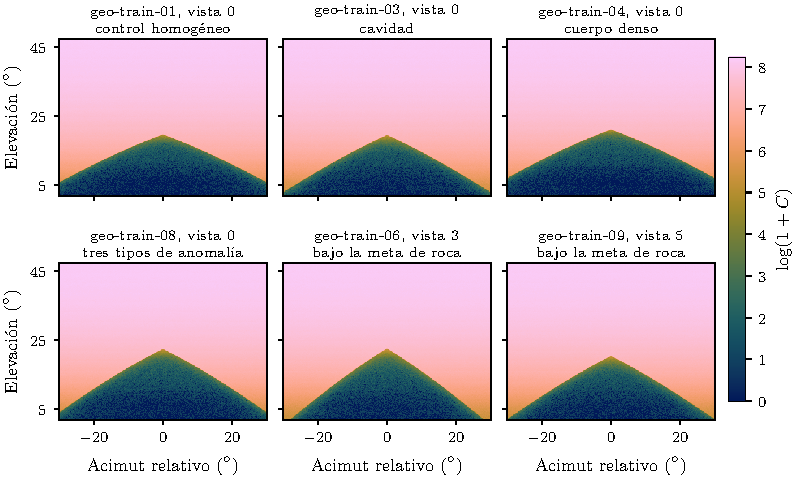
\includegraphics{fig4-1_referencias.pdf}
\caption[Seis referencias de la campaña de 114 vistas]{Seis referencias de la campaña de 114 vistas, en la escala común $\log(1+C)$, donde $C$ es el conteo del píxel, sin suavizado. Las vistas se eligieron para ilustrar casos y no constituyen una muestra estadística; las siluetas no son mapas de densidad. Fuente: elaboración propia a partir de las imágenes exportadas de la campaña, verificadas contra su inventario de huellas.}
\label{fig:res-referencias}
\end{figure}

\subsection{Respuesta en los bordes de la ventana}
\label{subsec:res-bordes}

Las 1\,710 regiones de borde, quince por cada una de las 114 vistas, resultaron equivalentes según el criterio de la \cref{eq:bordes}: el intervalo completo de su contraste quedó dentro de $\pm1$ punto porcentual, con una cobertura simultánea de la familia de al menos 95\,\%. La \cref{fig:res-bordes} presenta los 1\,710 intervalos agrupados por región. El extremo más alejado de cero fue de 0,933 puntos porcentuales, en la columna~2 de la vista~5 de geo-train-02. Los intervalos de las filas superiores son más estrechos que los de las columnas laterales, porque cada fila abarca toda la anchura de la ventana a la mayor elevación y reúne, por ello, más muones que una columna restringida a la banda de cielo de 30° a 42°.

\begin{figure}[htbp]
\centering
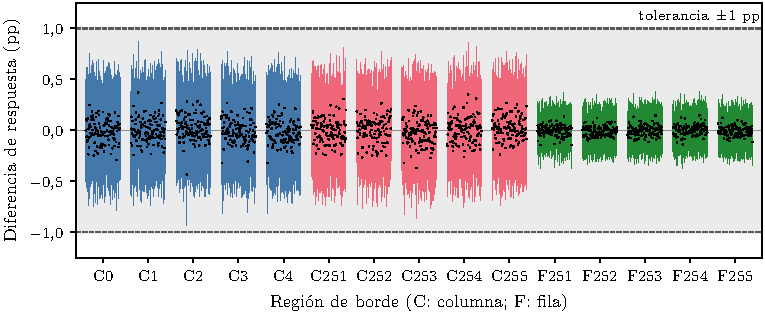
\includegraphics{fig4-2_bordes.pdf}
\caption[Respuesta en las regiones de borde de las 114 vistas]{Intervalos simultáneos del contraste de respuesta $\Delta_r$ (\cref{eq:bordes}) en las quince regiones de borde de cada una de las 114 vistas, en puntos porcentuales: columnas extremas izquierdas (C0 a C4) y derechas (C251 a C255) y filas superiores (F251 a F255). Cada segmento es una vista y cada punto, su estimación central; la franja gris marca la tolerancia de $\pm1$ punto porcentual. Fuente: elaboración propia a partir de la evaluación de la campaña.}
\label{fig:res-bordes}
\end{figure}

\subsection{Suficiencia del conteo en roca}
\label{subsec:res-roca}

El indicador descriptivo de la \cref{eq:roca} alcanzó la meta de 0,90 en 107 de las 114 vistas. La \cref{fig:res-roca} lo presenta por geometría y vista y lo relaciona con el número de regiones de roca de cada vista. Por vista, la fracción de regiones con al menos 100 cuentas varió entre 0,892 y 1,000, con una mediana de 0,961; la mediana de cuentas por región, entre 190 y 260,5, y el percentil 10, entre 97,2 y 157,5. Sobre el total de la campaña, 20\,713 de las 21\,816 regiones evaluadas alcanzaron 100 cuentas, es decir, el 94,944\,\%. Esa proporción global es descriptiva: no sustituye el indicador por vista ni convierte las siete excepciones en cumplimientos.

\begin{figure}[htbp]
\centering
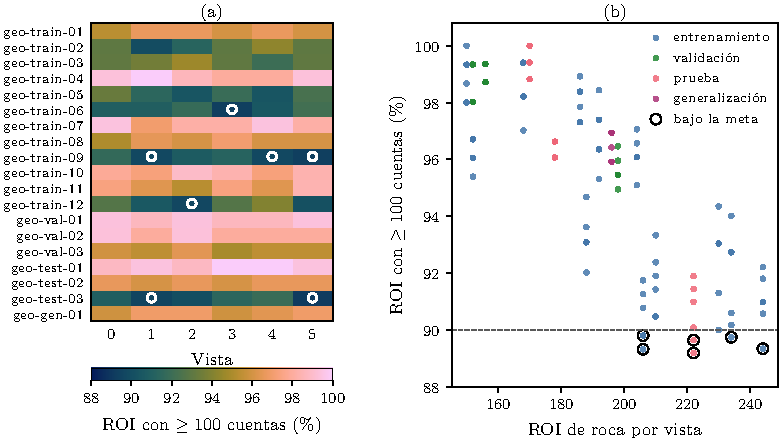
\includegraphics{fig4-3_roca.pdf}
\caption[Suficiencia del conteo en roca por vista]{Indicador descriptivo de suficiencia del conteo en roca (\cref{eq:roca}). (a)~Porcentaje de regiones de roca de $4\times4$ píxeles con al menos 100 cuentas, por geometría y vista; los círculos señalan las vistas por debajo de la meta del 90\,\%. (b)~El mismo porcentaje frente al número de regiones de roca de la vista, por partición; la línea discontinua marca la meta. Fuente: elaboración propia a partir de la evaluación de la campaña.}
\label{fig:res-roca}
\end{figure}

Las siete vistas por debajo de la meta, que la \cref{tab:excepciones} detalla, se conservaron sin cambios, conforme al acuerdo previo: no se aumentó el número de primarios, no se descartaron imágenes ni se modificó la regla después de conocer los resultados. Las siete comparten tres rasgos documentados. En primer lugar, todas quedaron a una o dos regiones de alcanzar la meta: con entre 206 y 244 regiones por vista, les faltaron una o dos regiones con 100 cuentas para llegar al 90\,\%. En segundo lugar, su percentil 10 se situó entre 97,2 y 100,0 cuentas, es decir, el déficit se concentra en un pequeño grupo de regiones con conteos próximos al umbral, y no en regiones sin señal. En tercer lugar, pertenecen a cuatro de las seis geometrías con más regiones de roca por vista, entre 206 y 244 frente a una mediana de 192 en el catálogo, lo que indica una mayor extensión de la banda de espesor nominal evaluada. Ese último rasgo no basta como explicación, porque las otras dos geometrías de ese grupo, geo-train-02, con 230 regiones, y geo-train-05, con 210, alcanzaron la meta en sus seis vistas, con mínimos de 0,900 y 0,905. El repositorio no establece una causa física individual para cada excepción; su cercanía al umbral es compatible con las fluctuaciones de conteo de las regiones próximas a 100 cuentas, sin que esa compatibilidad se haya demostrado con un análisis específico.

\begin{table}[htbp]
\centering
\caption[Vistas por debajo de la meta descriptiva de roca]{Vistas por debajo de la meta descriptiva de roca. $M_v$: regiones de roca de la vista; $n_{\geq100}$: regiones con al menos 100 cuentas; $F_v$: indicador de la \cref{eq:roca}; faltan: regiones adicionales necesarias para alcanzar $F_v\geq0{,}90$. Fuente: elaboración propia a partir de la evaluación de la campaña.}
\label{tab:excepciones}
\small
\begin{tabular}{@{}lrrrrrrr@{}}
\toprule
Geometría & Vista & $M_v$ & $n_{\geq100}$ & $F_v$ & Faltan & Mediana & Percentil 10 \\
\midrule
geo-test-03 & 1 & 222 & 199 & 0,896 & 1 & 205,5 & 99,1 \\
geo-test-03 & 5 & 222 & 198 & 0,892 & 2 & 201,0 & 97,2 \\
geo-train-06 & 3 & 244 & 218 & 0,893 & 2 & 206,0 & 99,0 \\
geo-train-09 & 1 & 206 & 185 & 0,898 & 1 & 191,5 & 99,5 \\
geo-train-09 & 4 & 206 & 185 & 0,898 & 1 & 194,5 & 100,0 \\
geo-train-09 & 5 & 206 & 184 & 0,893 & 2 & 194,0 & 99,0 \\
geo-train-12 & 2 & 234 & 210 & 0,897 & 1 & 195,5 & 99,3 \\
\bottomrule
\end{tabular}
\end{table}

La proyección previa a la campaña estimaba una fracción media de 89,7 a 91,1\,\%, mientras que la mediana observada por vista fue de 96,1\,\%. La comparación debe leerse con cautela, porque aquella proyección se calculó solo con las tasas de geo-train-06, una de las geometrías con más regiones de roca, y no con el promedio de las diecinueve.

\subsection{Discusión}
\label{subsec:res-discusion-oe1}

El producto obtenido es un conjunto de imágenes de conteo direccional sintético de muones primarios transmitidos a través de diecinueve escenarios volcánicos idealizados, observados desde seis direcciones, con referencias de $3{,}44\times10^{8}$ primarios y realizaciones de menor conteo en cuatro niveles de estadística. Cada píxel de una referencia cuenta los muones que alcanzaron el plano de conteo con energía superior a 3~GeV en una dirección dada; su forma adimensional es la transmisión direccional, que es la magnitud que la muografía por transmisión invierte para estimar la opacidad \parencite{lesparre2010,tanaka2023muography}. Los resultados de integridad y de reproducción muestran que ese producto está completo, que sus archivos no se alteraron y que el posproceso y la reducción de conteos se repiten exactamente desde los datos conservados. El resultado de bordes indica que, con la inyección junto a la roca y el margen de generación de 5°, la respuesta en los extremos de la ventana no difiere de la del interior en más de un punto porcentual respecto de la fuente ideal, lo que descarta un déficit sistemático de migración angular de esa magnitud en las 114 vistas. El indicador de roca, por su parte, describe que la mayoría de las regiones de roca evaluadas superan las 100 cuentas, lo que acota el ruido relativo de conteo en esas regiones agregadas a un orden del 10\,\% o menos.

Ese producto corresponde a la formulación del OE1 dentro del alcance idealizado adoptado: contiene imágenes sintéticas de transmisión, obtenidas por simulación Monte Carlo, de escenarios que representan una familia de edificios cónicos con conductos, cavidades y cuerpos densos, con diferentes niveles de estadística de conteo y una partición que impide la mezcla de variantes de una misma geometría entre entrenamiento y evaluación. La representatividad se sostiene dentro de esa familia, en los términos de la sección~\ref{subsec:met-geometrias}, y su valoración académica corresponde a la dirección.

Varias limitaciones acotan la interpretación física. La fuente híbrida y su extensión son hipótesis comunes del conjunto, y el espectro de EcoMug es más blando que el de la parametrización de Guan. El transporte sigue únicamente primarios, sin secundarios, respuesta instrumental ni fondo. El plano de conteo es una superficie computacional: dado que solo una fracción de entre el 3,6 y el 70,4\,\% de sus registros cae en el panel de 1,2~m, la imagen no puede identificarse con la de ese detector sin el control de equivalencia que no se ejecutó. La exposición es una escala convencional, y la referencia ideal de cielo con la que se evaluaron los bordes no incluye pérdidas en el aire, desintegración, dispersión ni migración angular, de modo que el contraste de bordes mide la no uniformidad respecto de esa referencia sin aislar su causa. El control de bordes de los ensayos cortos, que quedó abierto con su definición estricta, y el criterio de bordes de la campaña son magnitudes distintas, y sus máximos no deben compararse como si lo fueran. Con el umbral de 3~GeV, el conteo en roca de los controles fue de 0,57 a 0,85 veces la expectativa del frenado continuo, una diferencia que no se analizó. Además, las referencias conservan su propio ruido, las realizaciones de una vista comparten su referencia y no equivalen a simulaciones independientes de alta estadística, y las máscaras de roca ignoran las anomalías.

Quedan, por tanto, sin demostrar la equivalencia con un detector físico, una escala de flujo o de tiempo calibrada, la generalización de las imágenes a volcanes reales y cualquier capacidad de reconstrucción de densidad, que estas pruebas no abordan. Tampoco se realizó una segunda ejecución independiente del transporte en Geant4: la reproducción verificada comprende el posproceso desde los histogramas y la construcción de los pares, no el transporte. La conversión del conjunto al formato de entrenamiento de los objetivos siguientes no forma parte de los resultados del OE1 y no fue auditada en su revisión.

% =============================================================================
\section{Modelo de recuperación de imágenes de baja estadística (OE2)}
\label{sec:res-oe2}

Esta sección presenta los resultados de los ensayos de desarrollo, obtenidos sobre la partición de validación, y los de la evaluación final de las ocho redes congeladas sobre las particiones reservadas. Todas las cifras proceden de los informes, registros y evaluaciones conservados en el repositorio de referencia; las de la evaluación final incorporan la corrección numérica C2 del contraste y se contrastaron con la revisión de la dirección, que recalculó las métricas desde las predicciones. Conforme a la sección~\ref{subsec:met-protocolo}, los resultados de la evaluación final constituyen una \emph{evaluación descriptiva sobre datos potencialmente expuestos}: ninguna de las redes usó las particiones reservadas para entrenarse o seleccionarse, pero esas escenas ya se habían evaluado en una etapa anterior del proyecto con modelos de la misma arquitectura, de modo que los resultados no constituyen una confirmación independiente.

\subsection{Resultados de los ensayos de desarrollo}
\label{subsec:res-ensayos-oe2}

La \cref{tab:res-ensayos} reúne las métricas de validación de los ensayos de desarrollo, con la fracción 0,05 y los 360 pares de las tres geometrías de validación. En el piloto, ambas redes completaron su entrenamiento por parada temprana, después de doce épocas la U-Net y de trece la cGAN, y en las dos el mayor SSIM de validación se alcanzó en la época~5. En una GPU L40S, la época de la U-Net duró 16,2~s y la de la cGAN 86,7~s, diferencia atribuible a las cinco actualizaciones del crítico por cada una del generador. Las dos redes aumentaron el SSIM y el PSNR respecto de la entrada en las dieciocho referencias de validación; la cGAN, sin embargo, quedó por debajo de la U-Net en las dieciocho, con diferencias medias de $-0{,}0209$ en SSIM y de $-1{,}80$~dB en PSNR. Conforme a su protocolo, el piloto concluyó que la implementación funcionaba correctamente y que la aportación de la componente antagónica a la calidad era inconclusa.

\begin{table}[htbp]
\centering
\caption[Métricas de validación de los ensayos de desarrollo del OE2]{Métricas de validación de los ensayos de desarrollo del OE2 ($f=0{,}05$; 360 pares de tres geometrías). $Q$, cielo y borde en porcentaje de las cuentas de referencia; el contraste es el error absoluto medio sobre 23 combinaciones comunes de anomalía y vista. PSNR en dB. A: U-Net con L1; B: A con pérdida regional; C0 y C1: variantes de cada pareja (sección~\ref{subsec:met-entrenamiento}). La última columna (Ctrl.) indica los controles cumplidos por la variante B o C1 frente a su control. Fuente: elaboración propia a partir de los informes de los ensayos y de las revisiones de la dirección en el repositorio de referencia.}
\label{tab:res-ensayos}
\footnotesize
\setlength{\tabcolsep}{3.5pt}
\begin{tabular}{@{}llrrrrrrc@{}}
\toprule
Ensayo & Var. & $Q$ & Cielo & Borde & Contr. & SSIM & PSNR & Ctrl. \\
\midrule
-- & Entrada & 1,814 & 6,802 & 12,092 & 0,2464 & 0,75181 & 24,168 & -- \\
Piloto & U-Net & 21,896 & 4,22 & 7,323 & 0,0874 & 0,84367 & 32,904 & -- \\
Piloto & cGAN & 12,340 & 12,648 & 14,419 & 0,0907 & 0,82279 & 31,104 & -- \\
\midrule
Ajuste U-Net & A & 13,287 & 1,777 & 5,138 & 0,0868 & 0,84297 & 32,819 & \\
 & B & 11,239 & 1,686 & 5,699 & 0,0834 & 0,84306 & 32,769 & 6/8 \\
\midrule
Cont.~cGAN & C0 & 7,204 & 2,830 & 11,278 & 0,1052 & 0,81487 & 30,572 & \\
 & C1 & 4,765 & 2,238 & 11,265 & 0,0913 & 0,81570 & 30,646 & 8/8 \\
\midrule
R1 & C0 & 13,841 & 2,766 & 10,882 & 0,1407 & 0,81420 & 30,503 &  \\
 & C1 & 5,711 & 2,346 & 11,448 & 0,0870 & 0,81648 & 30,667 & 7/8 \\
R2 & C0 & 10,300 & 2,575 & 10,652 & 0,0954 & 0,81568 & 30,530 &  \\
 & C1 & 9,434 & 2,634 & 11,121 & 0,0782 & 0,81623 & 30,636 & 5/8 \\
R3 & C0 & 5,871 & 2,415 & 10,882 & 0,0994 & 0,81694 & 30,706 &  \\
 & C1 & 7,700 & 2,657 & 10,967 & 0,1032 & 0,81486 & 30,546 & 1/8 \\
\midrule
E1, B1 & C0 & 6,233 & 2,478 & 11,146 & 0,1157 & 0,81572 & 30,646 &  \\
 & C1 & 4,802 & 2,490 & 6,891 & 0,0866 & 0,81578 & 30,637 & 6/9 \\
E1, B2 & C0 & 7,812 & 2,468 & 11,263 & 0,0782 & 0,81456 & 30,526 &  \\
 & C1 & 7,158 & 2,319 & 7,045 & 0,0960 & 0,81495 & 30,588 & 7/9 \\
E1, B3 & C0 & 5,018 & 2,343 & 11,052 & 0,0868 & 0,81512 & 30,612 &  \\
 & C1 & 5,486 & 2,270 & 7,084 & 0,0783 & 0,81480 & 30,562 & 5/9 \\
\bottomrule
\end{tabular}
\end{table}

El diagnóstico regional de los modelos del piloto mostró que la ventaja en SSIM y PSNR no implicaba conservar las cuentas. La U-Net subestimó en un 16,97\,\% las cuentas de la roca sin anomalía, en un 36,07\,\% las de las cavidades y en un 59,96\,\% las del cuerpo denso, mientras que la cGAN, con sesgos de $-4{,}89$, $-26{,}02$ y $-32{,}08\,\%$ en esas regiones, sobreestimó en un 12,60\,\% las del cielo. La entrada sin red, por construcción, mantuvo esos sesgos por debajo del 3,2\,\% en valor absoluto, aunque con errores píxel a píxel muy superiores. En términos del indicador regional, $Q$ pasó de 1,814\,\% en la entrada a 21,896\,\% en la U-Net y a 12,340\,\% en la cGAN. Este hallazgo motivó los ensayos de ajuste.

En el ajuste de la U-Net, la variante con pérdida regional redujo $Q$ de 13,287 a 11,239\,\% y lo mejoró en las tres geometrías, pero empeoró el error de borde en las dieciocho vistas y redujo el PSNR en 0,050~dB, por lo que cumplió seis de los ocho controles y se clasificó como compromiso. El control sin término regional ya había reducido $Q$ desde el 21,896\,\% de la U-Net inicial hasta el 13,287\,\%, lo que indica que buena parte de la mejora procedía de continuar el entrenamiento con una tasa de aprendizaje menor y no del término regional. En la continuación de la cGAN, la variante C1 cumplió los ocho controles y redujo $Q$ en un 33,85\,\% respecto de C0, pero ambas quedaron por debajo de la cGAN inicial en SSIM y PSNR, la mejora del error de borde fue de solo 0,014 puntos porcentuales y $Q$ en geo-val-01 empeoró frente a la cGAN inicial, de 3,470 a 6,647\,\%. Con una sola semilla, el resultado se consideró una hipótesis por confirmar.

La repetición con tres semillas no confirmó esa ventaja. La variante C1 redujo $Q$ en dos de las tres parejas, con diferencias de $-8{,}130$, $-0{,}866$ y $+1{,}829$ puntos porcentuales, y empeoró el error de borde en las tres, entre $+0{,}085$ y $+0{,}566$ puntos; las parejas cumplieron siete, cinco y uno de los ocho controles, de modo que ninguna fue concordante y el resultado se clasificó como dependiente de la semilla o de compromiso. Además, el $Q$ del control C0 varió entre 5,871 y 13,841\,\% según la semilla, una dispersión del mismo orden que la diferencia entre variantes. Un diagnóstico espacial posterior explicó parte de este comportamiento: el término regional compara cuentas medias por región y es, por tanto, invariante ante redistribuciones de las cuentas que conserven su suma. En 40 de las 54 combinaciones de pareja y vista, el error de la cuenta total del borde disminuyó mientras su error píxel a píxel aumentaba.

El ensayo de borde E1 añadió, por ello, el término espacial de la \cref{eq:perdida-borde}. El error espacial de borde bajó de 11,146 a 6,891\,\%, de 11,263 a 7,045\,\% y de 11,052 a 7,084\,\% en las tres parejas, es decir, entre un 35,90 y un 38,17\,\%, y la reducción se repitió en las 54 combinaciones de pareja y vista, con disminuciones de entre 3,42 y 4,88 puntos porcentuales. Los demás indicadores no mejoraron de forma simultánea: $Q$ bajó en dos parejas y subió en la tercera, con diferencias de $-1{,}431$, $-0{,}653$ y $+0{,}468$ puntos, y en geo-val-01 empeoró en las tres, entre $+0{,}98$ y $+3{,}61$ puntos; el cielo, el contraste, el SSIM y el PSNR cambiaron de signo según la pareja. Ninguna pareja cumplió los nueve controles, y el ensayo se clasificó como compromiso. En geo-val-01, el sesgo de C1 aumentó en la roca y en el conducto, y el del conducto procedió casi por completo de los píxeles situados a más de ocho píxeles del borde, que reúnen el 99,5\,\% de sus cuentas; el término de borde corrigió, por tanto, la transición entre roca y cielo sin resolver el sesgo del interior. Una reproducción independiente en procesador de ese diagnóstico, con 252 sesgos, 126 filas regionales y 378 filas por banda de distancia, coincidió con el original con una diferencia máxima de $1{,}1\times10^{-16}$.

En todos los ensayos por continuación, la aceptación técnica confirmó la recuperación exacta de los entrenamientos interrumpidos y las predicciones obtenidas en GPU se reprodujeron en procesador con diferencias por píxel inferiores a $10^{-5}$. Las particiones de prueba y de generalización no se abrieron en ninguno de ellos.

\subsection{Integridad de la evaluación final}
\label{subsec:res-integridad-ef}

La evaluación final se ejecutó en una GPU L40S con el código y los pesos fijados en su contrato, que superaron la comprobación previa de huellas sin abrir ninguna matriz. La inferencia de las 480 imágenes de cada red duró entre 3,5 y 17,8~s, y la evaluación conjunta en procesador, 44~s. Se obtuvieron 4\,320 registros de imagen, 480 por método, 1\,134 registros regionales y 54 combinaciones de contraste, de las cuales 48 fueron estimables y seis no reunieron el soporte geométrico mínimo. Ninguna región quedó como no estimable y el indicador $Q$ resultó completo en las cuatro geometrías. La revisión de la dirección verificó las 32 matrices de predicciones contra sus huellas, recalculó todas las métricas desde ellas con los resultados descritos en la sección~\ref{subsec:met-reproduccion} y estableció la corrección C2 de la selección de controles de contraste, que modificó ocho contrastes de referencia y conservó exactamente el SSIM, el PSNR y los indicadores regionales. Las cifras que siguen incorporan esa corrección.

\subsection{Calidad global de imagen y conservación de cuentas}
\label{subsec:res-global}

La \cref{tab:res-ef01} presenta los macropromedios de la evaluación final para los nueve métodos y las dos particiones. En prueba, la cGAN original aumentó el SSIM de 0,7643 a 0,8342 y el PSNR de 24,258 a 31,170~dB respecto de la entrada, y la U-Net alcanzó 0,8545 y 33,074~dB. Sin embargo, el indicador regional $Q$ aumentó de 1,832\,\% en la entrada a 14,566\,\% en la cGAN y a 22,388\,\% en la U-Net. Conviene recordar que $Q$ resume el sesgo de cuentas en las regiones definidas (\cref{eq:regiones-q}); no representa un error de densidad ni un porcentaje de error de toda la imagen. Las continuaciones del ensayo de borde redujeron $Q$ respecto de las redes originales, con valores entre 3,996 y 5,825\,\% en prueba, a costa de métricas de imagen inferiores a las de la U-Net. En generalización se repitió el mismo patrón: la entrada obtuvo 0,7502, 23,904~dB y un $Q$ de 1,093\,\%; la U-Net, 0,8454, 32,883~dB y 26,505\,\%, y la cGAN, 0,8252, 31,047~dB y 16,959\,\%, mientras que las continuaciones mantuvieron $Q$ entre 2,271 y 4,755\,\%. La cGAN original presentó, además, el mayor error en el cielo, de 15,37\,\% en prueba frente a 6,84\,\% en la entrada.

\begin{table}[htbp]
\centering
\caption[Resultados globales de la evaluación final]{Macropromedios de la evaluación final EF-01 con $f=0{,}05$, con igual peso por geometría. $Q$, cielo y borde en porcentaje de las cuentas de referencia. Evaluación descriptiva sobre datos potencialmente expuestos. Fuente: elaboración propia a partir de los resultados corregidos (C2) de la evaluación final en el repositorio de referencia.}
\label{tab:res-ef01}
\small
\begin{tabular}{@{}lrrrrr@{}}
\toprule
Método & SSIM & PSNR (dB) & $Q$ (\%) & Cielo (\%) & Borde (\%) \\
\midrule
\multicolumn{6}{@{}l}{\emph{Prueba}} \\
Entrada sin red & 0{,}7643 & 24{,}258 & 1{,}832 & 6{,}84 & 12{,}38 \\
U-Net original & 0{,}8545 & 33{,}074 & 22{,}388 & 4{,}82 & 6{,}96 \\
cGAN original & 0{,}8342 & 31{,}170 & 14{,}566 & 15{,}37 & 14{,}13 \\
B1 -- C0 & 0{,}8277 & 30{,}839 & 5{,}825 & 3{,}29 & 11{,}11 \\
B1 -- C1 & 0{,}8278 & 30{,}849 & 4{,}821 & 2{,}81 & 7{,}14 \\
B2 -- C0 & 0{,}8274 & 30{,}772 & 3{,}996 & 2{,}43 & 11{,}35 \\
B2 -- C1 & 0{,}8273 & 30{,}770 & 4{,}727 & 2{,}35 & 7{,}10 \\
B3 -- C0 & 0{,}8263 & 30{,}729 & 4{,}828 & 2{,}86 & 11{,}57 \\
B3 -- C1 & 0{,}8273 & 30{,}768 & 5{,}480 & 2{,}39 & 7{,}34 \\
\midrule
\multicolumn{6}{@{}l}{\emph{Generalización}} \\
Entrada sin red & 0{,}7502 & 23{,}904 & 1{,}093 & 6{,}81 & 12{,}00 \\
U-Net original & 0{,}8454 & 32{,}883 & 26{,}505 & 4{,}67 & 6{,}66 \\
cGAN original & 0{,}8252 & 31{,}047 & 16{,}959 & 14{,}55 & 13{,}40 \\
B1 -- C0 & 0{,}8161 & 30{,}485 & 3{,}808 & 3{,}10 & 10{,}29 \\
B1 -- C1 & 0{,}8151 & 30{,}509 & 4{,}323 & 2{,}26 & 6{,}60 \\
B2 -- C0 & 0{,}8145 & 30{,}331 & 4{,}131 & 2{,}16 & 10{,}65 \\
B2 -- C1 & 0{,}8154 & 30{,}403 & 4{,}755 & 2{,}14 & 6{,}65 \\
B3 -- C0 & 0{,}8149 & 30{,}404 & 4{,}054 & 2{,}53 & 10{,}55 \\
B3 -- C1 & 0{,}8146 & 30{,}371 & 2{,}271 & 2{,}14 & 6{,}88 \\
\bottomrule
\end{tabular}
\end{table}

La \cref{fig:compromiso} sitúa los nueve métodos en el plano formado por cada métrica de imagen y el indicador regional, y muestra el resultado central de la evaluación: ningún método ocupa la región deseable de alta similitud y bajo sesgo. La entrada conserva las cuentas, pero con la menor similitud; las redes originales ganan similitud a costa del sesgo regional, y las continuaciones ocupan una posición intermedia, con una pérdida de similitud reducida respecto de la cGAN y un sesgo cercano al de la entrada.

\begin{figure}[htbp]
\centering
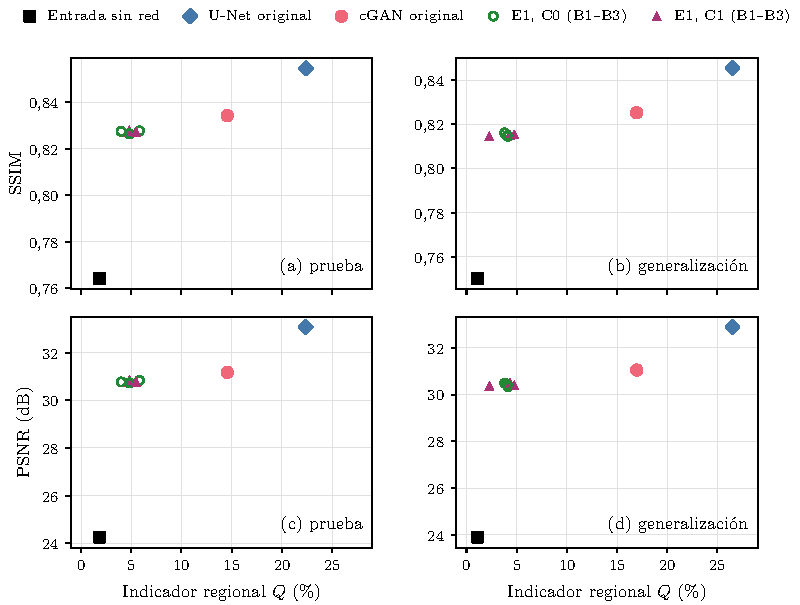
\includegraphics{fig4-4_compromiso.pdf}
\caption[Compromiso entre similitud de imagen y conservación de cuentas]{Compromiso entre similitud de imagen y conservación de cuentas en la evaluación final: SSIM (a, b) y PSNR (c, d) frente al indicador regional $Q$, en prueba (a, c) y en generalización (b, d). Cada símbolo es un macropromedio por partición; las seis variantes del ensayo de borde se muestran completas, sin seleccionar semillas. Evaluación descriptiva sobre datos potencialmente expuestos. Fuente: elaboración propia a partir de los resultados corregidos (C2) de la evaluación final en el repositorio de referencia.}
\label{fig:compromiso}
\end{figure}

La \cref{fig:comparacion-fija} ilustra estos resultados sobre imágenes concretas. Para no seleccionar casos favorables, se fijaron por índice la vista~0 y la realización~0 de cada geometría reservada, y los dieciséis paneles comparten una misma escala en el dominio normalizado de la \cref{eq:norm-v1}, sin ajustarla por imagen. La entrada al 5\,\% muestra el ruido de conteo, que es más visible en la roca; la U-Net produce imágenes suaves, con un oscurecimiento del interior del edificio coherente con su subestimación de las cuentas de la roca, y la cGAN conserva una textura más próxima a la de la referencia. Ninguna de esas apariencias constituye por sí sola evidencia de recuperación física: deben interpretarse junto con los indicadores regionales de la \cref{tab:res-ef01}.

\begin{figure}[htbp]
\centering
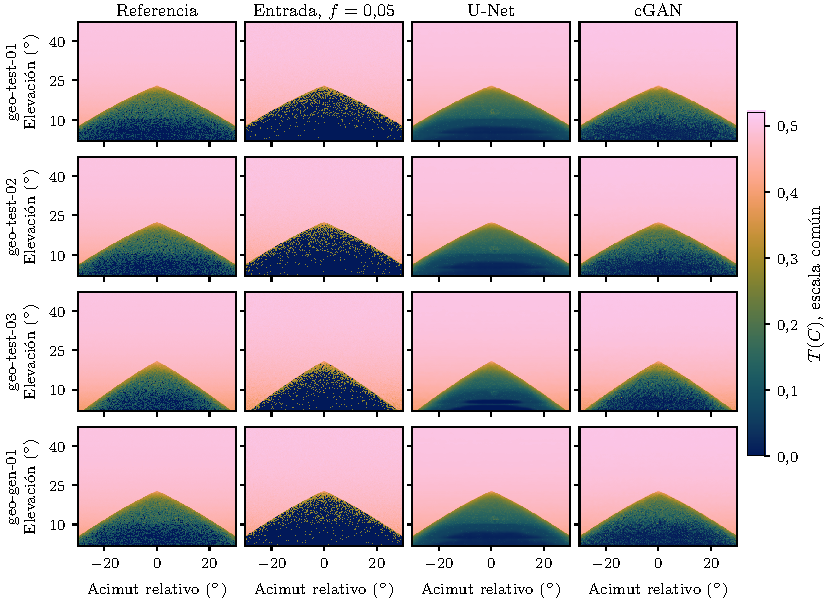
\includegraphics{fig4-7_comparacion_fija.pdf}
\caption[Comparación de imágenes en las cuatro geometrías reservadas]{Comparación de imágenes en las cuatro geometrías reservadas: referencia de alta estadística, entrada con $f=0{,}05$ y salidas de la U-Net y de la cGAN originales, para la vista~0 y la realización~0 de cada geometría, fijadas por índice. Todas las imágenes se representan en el dominio normalizado $T(C)$ de la \cref{eq:norm-v1}, con una escala común a los dieciséis paneles; las matrices se muestran a su resolución nativa de $256\times256$ píxeles, sin interpolación. Evaluación descriptiva sobre datos potencialmente expuestos. Fuente: elaboración propia a partir de las predicciones conservadas de la evaluación final, con la regla de selección del informe de la dirección.}
\label{fig:comparacion-fija}
\end{figure}

Para mostrar de forma explícita una limitación, la \cref{fig:caso-desfavorable} toma la geometría con el mayor indicador regional de la cGAN original entre las cuatro reservadas, geo-test-03, con un $Q$ de 27,835\,\%, y conserva la misma vista y realización. La regla se basa en el indicador agregado de la geometría y no en la búsqueda de la imagen visualmente más desfavorable. La figura incluye las seis continuaciones y los residuos de los nueve métodos respecto de la referencia, con una escala común y simétrica. El residuo de la entrada está dominado por el ruido de conteo de la roca, mientras que los de las redes tienen menor amplitud, pero no se anulan en el interior del edificio. Los residuos se expresan en $T(C)$ y no representan directamente sesgos de cuentas ni errores de densidad, y el valor de $Q$ citado corresponde a la geometría completa y no al panel mostrado. Esta comparación es posterior a la evaluación y tiene carácter ilustrativo.

\begin{figure}[htbp]
\centering
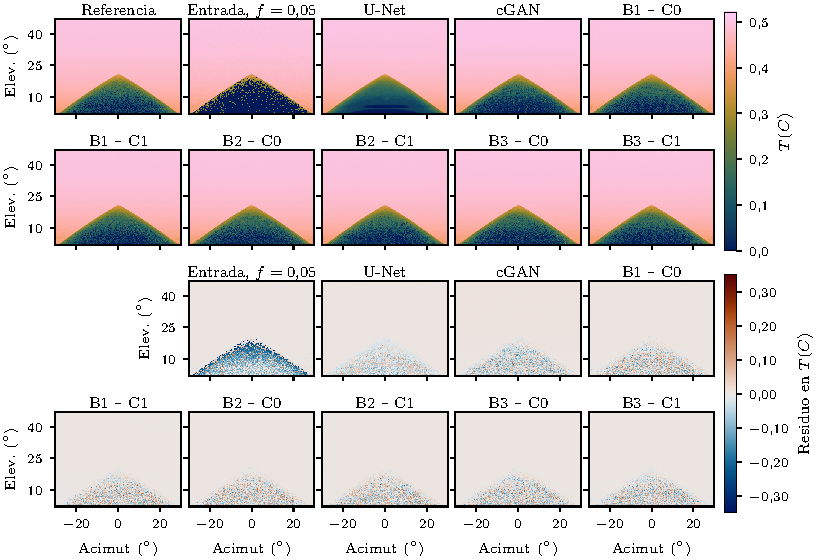
\includegraphics{fig4-8_caso_desfavorable.pdf}
\caption[Caso desfavorable: imágenes y residuos de todos los modelos]{Caso desfavorable de la evaluación final: geo-test-03, la geometría con el mayor indicador regional de la cGAN original ($Q=27{,}835\,\%$), vista~0 y realización~0. Filas superiores: referencia, entrada y salidas de las ocho redes en $T(C)$, con la escala común de la \cref{fig:comparacion-fija}. Filas inferiores: residuo de cada método respecto de la referencia en $T(C)$, con una escala común y simétrica de $\pm0{,}350$. Comparación posterior a la evaluación, seleccionada con una regla descriptiva explícita; evaluación descriptiva sobre datos potencialmente expuestos. Fuente: elaboración propia a partir de las predicciones conservadas de la evaluación final, con la regla de selección del informe de la dirección.}
\label{fig:caso-desfavorable}
\end{figure}

\subsection{Error de borde y contraste de las anomalías}
\label{subsec:res-regiones}

La reducción del error espacial de borde observada en validación se repitió en las cuatro geometrías reservadas y en las tres parejas, como muestra la \cref{fig:borde}. En prueba, el término de borde redujo ese error entre 3,7 y 4,7 puntos porcentuales y, en generalización, entre 3,7 y 4,0 puntos; en términos relativos, entre un 31 y un 40\,\% en las doce combinaciones de pareja y geometría. Con el término de borde, las continuaciones alcanzaron errores de borde de 6,6 a 8,3\,\%, comparables a los de la U-Net, de 6,7 a 7,2\,\%, y muy inferiores a los de la cGAN original, de 13,4 a 14,5\,\%, que fue el único método con un error de borde mayor que el de la entrada.

\begin{figure}[htbp]
\centering
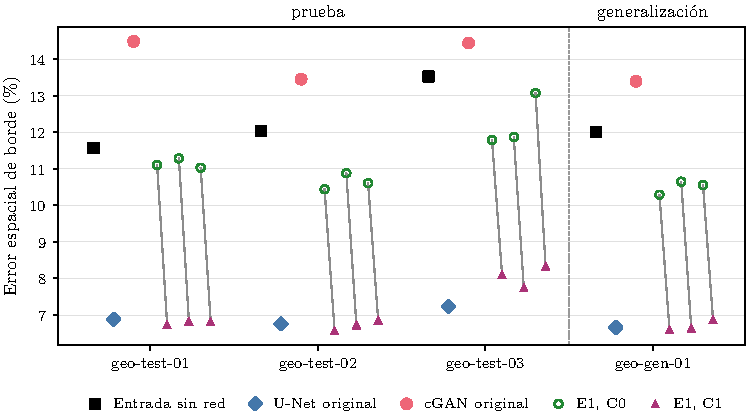
\includegraphics{fig4-5_borde.pdf}
\caption[Error espacial de borde por geometría en la evaluación final]{Error espacial de borde por geometría en la evaluación final. Para cada pareja B1--B3, el segmento une la variante C0, sin término de borde, con la variante C1, que lo incorpora. Evaluación descriptiva sobre datos potencialmente expuestos. Fuente: elaboración propia a partir de los resultados corregidos (C2) de la evaluación final en el repositorio de referencia.}
\label{fig:borde}
\end{figure}

La \cref{tab:contraste-c2} presenta el error de contraste antes y después de la corrección C2, sobre el soporte común de 30 combinaciones de anomalía y vista en prueba y de 16 en generalización. Todas las redes redujeron el error de contraste de la entrada, de 0,337 a entre 0,092 y 0,135 en prueba y de 0,290 a entre 0,072 y 0,115 en generalización, y la U-Net obtuvo el menor en ambas particiones. La corrección modificó los valores en menos de 0,005 en todos los casos salvo dos: la entrada en generalización, cuyo error pasó de 0,271327 a 0,289711, y una variante cuyo cambio altera la interpretación: en la pareja B1 sobre generalización, la variante C1 pasó de tener un error de contraste mayor que C0, de 0,137584 frente a 0,101319, a tener uno menor, de 0,090703 frente a 0,105524. Que una corrección numérica de la selección de controles invierta el signo de esa comparación indica que las diferencias de contraste entre variantes de una misma pareja, basadas en pocas combinaciones de una sola geometría, son sensibles a detalles del cálculo y no deben interpretarse como un efecto robusto del término de borde.

\begin{table}[htbp]
\centering
\caption[Error de contraste antes y después de la corrección C2]{Error absoluto medio de contraste (adimensional) en la evaluación final, con la selección original de controles y con la corrección numérica C2 de la selección de controles. Soporte común: 30 combinaciones de anomalía y vista en prueba y 16 en generalización. Fuente: elaboración propia a partir de la comparación antes y después de la revisión C2 en el repositorio de referencia.}
\label{tab:contraste-c2}
\small
\begin{tabular}{@{}lrrrr@{}}
\toprule
 & \multicolumn{2}{c}{Prueba} & \multicolumn{2}{c}{Generalización} \\
\cmidrule(lr){2-3}\cmidrule(l){4-5}
Método & Original & C2 & Original & C2 \\
\midrule
Entrada sin red & 0{,}336628 & 0{,}337054 & 0{,}271327 & 0{,}289711 \\
U-Net original & 0{,}093172 & 0{,}092463 & 0{,}072958 & 0{,}071503 \\
cGAN original & 0{,}135066 & 0{,}135104 & 0{,}088471 & 0{,}086302 \\
B1 -- C0 & 0{,}132899 & 0{,}133285 & 0{,}101319 & 0{,}105524 \\
B1 -- C1 & 0{,}100570 & 0{,}102743 & 0{,}137584 & 0{,}090703 \\
B2 -- C0 & 0{,}112721 & 0{,}112458 & 0{,}113495 & 0{,}114919 \\
B2 -- C1 & 0{,}108925 & 0{,}109112 & 0{,}099638 & 0{,}096729 \\
B3 -- C0 & 0{,}116936 & 0{,}116575 & 0{,}076043 & 0{,}073659 \\
B3 -- C1 & 0{,}127687 & 0{,}127915 & 0{,}077899 & 0{,}077246 \\
\bottomrule
\end{tabular}
\end{table}

\subsection{Comparaciones predeclaradas}
\label{subsec:res-comparaciones}

La \cref{tab:comparaciones} resume las doce comparaciones fijadas en el protocolo, seis por partición, con el número de geometrías en las que el candidato no empeoró cada métrica respecto de su comparador. Las doce se clasificaron como compromiso o deterioro conforme a la \cref{eq:clasificacion}, y ninguna cambió de clase con la corrección C2. La cGAN y la U-Net mejoraron el SSIM, el PSNR y el contraste de la entrada en todas las geometrías, pero aumentaron $Q$ en todas; la cGAN empeoró, además, los errores de cielo y de borde de la entrada. Frente a la U-Net, la cGAN solo mejoró $Q$. Dentro de las parejas del ensayo de borde, C1 mejoró los errores de cielo y de borde en todas las geometrías, mientras que $Q$, el contraste, el SSIM y el PSNR cambiaron de signo según la pareja y la geometría, con diferencias de SSIM no mayores de 0,002 y de PSNR no mayores de 0,12~dB. Ninguna clasificación implica significación ni superioridad estadística, y la elección de las semillas no se modificó después de abrir las particiones reservadas.

\begin{table}[htbp]
\centering
\caption[Comparaciones predeclaradas de la evaluación final]{Comparaciones predeclaradas de la evaluación final: número de geometrías en las que el candidato no empeoró cada métrica respecto del comparador (prueba: tres geometrías; generalización: una) y clasificación según la \cref{eq:clasificacion}. Fuente: elaboración propia a partir de los resultados corregidos (C2) de la evaluación final en el repositorio de referencia.}
\label{tab:comparaciones}
\footnotesize
\setlength{\tabcolsep}{4pt}
\begin{tabular}{@{}lrrrrrrl@{}}
\toprule
Comparación & SSIM & PSNR & $Q$ & Cielo & Borde & Contraste & Clase \\
\midrule
\multicolumn{8}{@{}l}{\emph{Prueba}} \\
cGAN frente a entrada & 3/3 & 3/3 & 0/3 & 0/3 & 0/3 & 3/3 & Compromiso o deterioro \\
U-Net frente a entrada & 3/3 & 3/3 & 0/3 & 3/3 & 3/3 & 3/3 & Compromiso o deterioro \\
cGAN frente a U-Net & 0/3 & 0/3 & 3/3 & 0/3 & 0/3 & 0/3 & Compromiso o deterioro \\
B1: C1 frente a C0 & 2/3 & 2/3 & 2/3 & 3/3 & 3/3 & 3/3 & Compromiso o deterioro \\
B2: C1 frente a C0 & 1/3 & 2/3 & 1/3 & 3/3 & 3/3 & 2/3 & Compromiso o deterioro \\
B3: C1 frente a C0 & 2/3 & 2/3 & 2/3 & 3/3 & 3/3 & 2/3 & Compromiso o deterioro \\
\midrule
\multicolumn{8}{@{}l}{\emph{Generalización}} \\
cGAN frente a entrada & 1/1 & 1/1 & 0/1 & 0/1 & 0/1 & 1/1 & Compromiso o deterioro \\
U-Net frente a entrada & 1/1 & 1/1 & 0/1 & 1/1 & 1/1 & 1/1 & Compromiso o deterioro \\
cGAN frente a U-Net & 0/1 & 0/1 & 1/1 & 0/1 & 0/1 & 0/1 & Compromiso o deterioro \\
B1: C1 frente a C0 & 0/1 & 1/1 & 0/1 & 1/1 & 1/1 & 1/1 & Compromiso o deterioro \\
B2: C1 frente a C0 & 1/1 & 1/1 & 0/1 & 1/1 & 1/1 & 1/1 & Compromiso o deterioro \\
B3: C1 frente a C0 & 0/1 & 0/1 & 1/1 & 1/1 & 1/1 & 0/1 & Compromiso o deterioro \\
\bottomrule
\end{tabular}
\end{table}

% =============================================================================
\section{Desempeño frente a la exposición (OE3)}
\label{sec:res-oe3}

Esta sección presenta el análisis descriptivo de la sección~\ref{subsec:met-factor}, que compara la entrada sin red con cuatro fracciones de conteo con las ocho redes evaluadas al 5\,\%. Como la evaluación final, se trata de un análisis posterior a la apertura de las reservas y sobre datos potencialmente expuestos, y no de una validación confirmatoria ni de una selección de modelos.

\subsection{Curvas descriptivas de exposición}
\label{subsec:res-curvas}

La \cref{tab:curvas} reúne las métricas de la entrada sin red con fracciones de 0,01, 0,05, 0,10 y 0,50 junto con las de las redes, y la \cref{fig:curvas} las representa frente a la fracción de conteos conservada. El caso de 0,05 reprodujo los valores de la entrada de la evaluación final con una tolerancia de $10^{-12}$. Como era de esperar, la calidad de la entrada mejoró de forma monótona con la fracción: en prueba, el SSIM pasó de 0,6959 al 1\,\% a 0,9250 al 50\,\%, el PSNR de 22,537 a 33,101~dB y $Q$ disminuyó de 2,897 a 0,437\,\%. El error de contraste se calculó sobre el soporte común a las cuatro fracciones y a las ocho redes, de 21 combinaciones en prueba y 11 en generalización, porque con la fracción 0,01 algunas realizaciones tienen controles sin cuentas; por ello, esos valores no son comparables con los de la \cref{tab:contraste-c2}.

\begin{table}[htbp]
\centering
\caption[Métricas de la entrada sin red con cuatro fracciones y de las redes al 5\,\%]{Métricas de la entrada sin red con cuatro fracciones de conteo y de las redes evaluadas con $f=0{,}05$. $Q$ en porcentaje de las cuentas de referencia; contraste sobre el soporte común de 21 combinaciones en prueba y 11 en generalización. Análisis descriptivo posterior sobre datos potencialmente expuestos. Fuente: elaboración propia a partir de las curvas descriptivas de exposición y de los resultados corregidos (C2) en el repositorio de referencia.}
\label{tab:curvas}
\small
\begin{tabular}{@{}lrrrr@{}}
\toprule
Método y fracción & SSIM & PSNR (dB) & $Q$ (\%) & Contraste \\
\midrule
\multicolumn{5}{@{}l}{\emph{Prueba}} \\
Entrada sin red, 1\,\% & 0{,}6959 & 22{,}537 & 2{,}897 & 0{,}504 \\
Entrada sin red, 5\,\% & 0{,}7643 & 24{,}258 & 1{,}832 & 0{,}164 \\
Entrada sin red, 10\,\% & 0{,}7964 & 25{,}722 & 1{,}334 & 0{,}111 \\
Entrada sin red, 50\,\% & 0{,}9250 & 33{,}101 & 0{,}437 & 0{,}034 \\
U-Net original, 5\,\% & 0{,}8545 & 33{,}074 & 22{,}388 & 0{,}070 \\
cGAN original, 5\,\% & 0{,}8342 & 31{,}170 & 14{,}566 & 0{,}077 \\
E1, seis variantes, 5\,\% & 0{,}8263--0{,}8278 & 30{,}729--30{,}849 & 3{,}996--5{,}825 & 0{,}065--0{,}074 \\
\midrule
\multicolumn{5}{@{}l}{\emph{Generalización}} \\
Entrada sin red, 1\,\% & 0{,}6851 & 22{,}299 & 3{,}067 & 0{,}569 \\
Entrada sin red, 5\,\% & 0{,}7502 & 23{,}904 & 1{,}093 & 0{,}159 \\
Entrada sin red, 10\,\% & 0{,}7834 & 25{,}349 & 0{,}895 & 0{,}119 \\
Entrada sin red, 50\,\% & 0{,}9197 & 32{,}752 & 0{,}449 & 0{,}040 \\
U-Net original, 5\,\% & 0{,}8454 & 32{,}883 & 26{,}505 & 0{,}066 \\
cGAN original, 5\,\% & 0{,}8252 & 31{,}047 & 16{,}959 & 0{,}079 \\
E1, seis variantes, 5\,\% & 0{,}8145--0{,}8161 & 30{,}331--30{,}509 & 2{,}271--4{,}755 & 0{,}067--0{,}095 \\
\bottomrule
\end{tabular}
\end{table}

\begin{figure}[htbp]
\centering
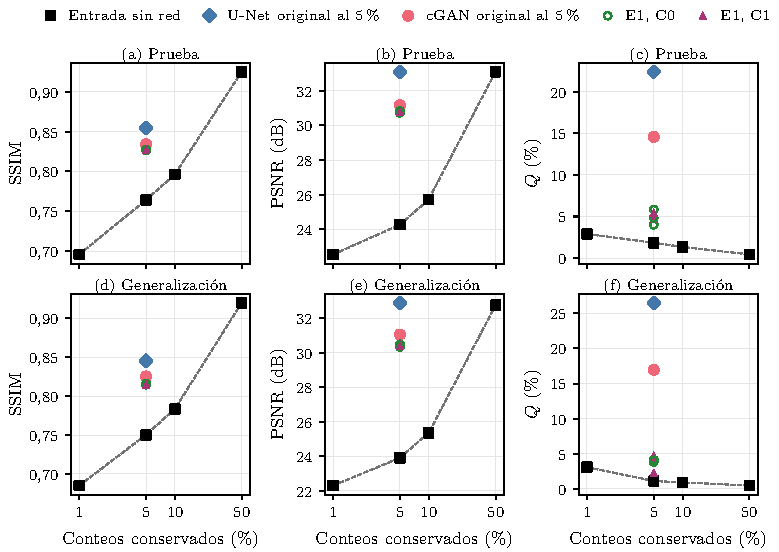
\includegraphics{fig4-6_curvas_exposicion.pdf}
\caption[Curvas descriptivas de exposición de la entrada sin red]{Curvas descriptivas de exposición: SSIM, PSNR e indicador regional $Q$ de la entrada sin red con cuatro fracciones de conteo, en prueba (a--c) y en generalización (d--f), junto con las ocho redes, evaluadas solo con la fracción 0,05. Las líneas discontinuas unen valores medidos como guía visual y no se usan para interpolar factores de adquisición. Análisis descriptivo posterior sobre datos potencialmente expuestos. Fuente: elaboración propia a partir de las curvas descriptivas de exposición y de los resultados corregidos (C2) en el repositorio de referencia.}
\label{fig:curvas}
\end{figure}

En prueba, la cGAN original al 5\,\% obtuvo un SSIM de 0,8342 y un PSNR de 31,170~dB, superiores a los de la entrada sin red al 10\,\%, de 0,7964 y 25,722~dB. La \cref{tab:cgan-10} muestra que esa relación no depende del promedio: se cumplió en cada una de las cuatro geometrías reservadas, tanto en SSIM como en PSNR, mientras que en todas ellas la cGAN quedó por debajo de la entrada al 50\,\%. Ambas métricas comparan cada imagen con la misma referencia de alta estadística, de modo que no comparan directamente la salida de la red con la entrada al 10\,\%. Sin embargo, $Q$ pasó de 1,334\,\% en esa entrada a 14,566\,\% en la cGAN: la mejora de similitud no implicó conservar mejor las cuentas.

\begin{table}[htbp]
\centering
\caption[cGAN al 5\,\% frente a la entrada sin red al 10\,\% por geometría]{SSIM y PSNR de la cGAN original con $f=0{,}05$ y de la entrada sin red con el 10\,\% de los conteos, por geometría reservada; ambas métricas se calculan frente a la misma referencia de alta estadística. Análisis descriptivo posterior sobre datos potencialmente expuestos. Fuente: elaboración propia a partir de los resultados corregidos (C2) y de las curvas descriptivas de exposición en el repositorio de referencia.}
\label{tab:cgan-10}
\small
\begin{tabular}{@{}lrrrr@{}}
\toprule
 & \multicolumn{2}{c}{SSIM} & \multicolumn{2}{c}{PSNR (dB)} \\
\cmidrule(lr){2-3}\cmidrule(l){4-5}
Geometría & cGAN, 5\,\% & Entrada, 10\,\% & cGAN, 5\,\% & Entrada, 10\,\% \\
\midrule
geo-test-01 & 0{,}8095 & 0{,}7667 & 30{,}900 & 25{,}240 \\
geo-test-02 & 0{,}8233 & 0{,}7822 & 31{,}107 & 25{,}468 \\
geo-test-03 & 0{,}8697 & 0{,}8403 & 31{,}504 & 26{,}458 \\
geo-gen-01 & 0{,}8252 & 0{,}7834 & 31{,}047 & 25{,}349 \\
\bottomrule
\end{tabular}
\end{table}

 Las seis continuaciones también superaron, en estos promedios, el SSIM y el PSNR de la entrada al 10\,\%, con un $Q$ de entre 3,996 y 5,825\,\% frente al 1,334\,\%, y la U-Net ofreció los mayores valores de similitud con el mayor $Q$. En los macropromedios de prueba, las ocho redes quedaron entre los valores de la entrada al 10 y al 50\,\% tanto en SSIM como en PSNR. En generalización ocurrió lo mismo, salvo que el PSNR de la U-Net superó ligeramente el de la entrada al 50\,\%, con 32,883 frente a 32,752~dB, aunque su SSIM permaneció por debajo. En contraste, las redes, con errores de 0,065 a 0,095, quedaron entre la entrada al 10\,\% y al 50\,\%. Estas diferencias no constituyen una prueba de superioridad estadística, porque las realizaciones de una misma geometría no se trataron como geometrías independientes, y los cruces por geometría de los demás modelos, que el análisis también registró, no deben sustituirse por los promedios.

\subsection{Razones nominales de exposición y alcance del factor de reducción}
\label{subsec:res-factor}

Según la \cref{eq:factor}, una red alimentada con $f_{\mathrm{mod}}=0{,}05$ y una entrada sin red con fracción $f_{\mathrm{ent}}$ guardan una razón nominal de exposiciones $R=f_{\mathrm{ent}}/0{,}05$, que vale 2 frente a la entrada al 10\,\%, 10 frente a la del 50\,\% y 20 frente a la referencia completa. Con esa equivalencia, los resultados anteriores indican que las redes al 5\,\% superan en SSIM y PSNR a una entrada con el doble de conteos, en el caso de la cGAN en cada una de las cuatro geometrías, con deterioro de la conservación regional de las cuentas, y que no alcanzan, salvo el PSNR de la U-Net en generalización, a la entrada con diez veces más conteos. La rejilla sitúa, por tanto, los cruces de las métricas de similitud entre los puntos asociados nominalmente a 2 y a 10; en el PSNR de la U-Net en generalización, el cruce queda fuera de la rejilla y no se extrapoló.

Estos resultados no permiten estimar un factor de reducción entre 2 y 10, un factor máximo alcanzable ni un intervalo de confianza, porque no hay mediciones intermedias, no se adoptó ninguna ley de interpolación y las redes solo se evaluaron con la fracción de 0,05. Tampoco el factor nominal de 20 asociado a $f=0{,}05$ es un factor alcanzado: describe la reducción de conteos de la entrada, no la calidad del resultado. Determinar el factor alcanzable exige un criterio de calidad aceptable, justificado por la aplicación o por una referencia científica externa, que separe la equivalencia descriptiva según SSIM y PSNR de la aceptación física según cuentas y contraste; como no se había fijado un criterio de calidad aceptable con un margen fundamentado, los resultados se informan como una comparación descriptiva por métrica, sin un factor único que oculte el deterioro de la conservación de cuentas, y el factor de reducción alcanzable no está demostrado. Las razones se refieren, además, a fracciones de conteos obtenidas por adelgazamiento de referencias idealizadas, y no a tiempos de adquisición medidos.

\subsection{Discusión}
\label{subsec:res-discusion-oe2}

Se implementó y entrenó un modelo generativo condicionado para recuperar imágenes muográficas a partir de una fracción de conteos de 0,05, y se comparó con una red U-Net entrenada con pérdida L1 y con la entrada de baja estadística escalada a cuentas equivalentes. La evaluación final incluyó tres geometrías de prueba y una de generalización, con seis vistas y veinte realizaciones por vista, y ocho redes previamente congeladas, entre ellas seis continuaciones destinadas a estudiar la conservación regional y el error de borde; estas continuaciones comparten la inicialización y no constituyen entrenamientos independientes desde cero.

El resultado central es un compromiso entre la similitud visual y la conservación de las cuentas. Todas las redes redujeron el ruido de conteo y aumentaron el SSIM y el PSNR de la entrada en las cuatro geometrías reservadas, pero ninguna mejoró todos los indicadores a la vez: las que más se acercaron a la referencia en esas métricas, la U-Net y, en menor medida, la cGAN, fueron también las que más desplazaron las cuentas de la roca y de las anomalías. La U-Net, entrenada solo con el término L1, superó a la cGAN original en SSIM y en PSNR en las dos particiones, de modo que la componente antagónica no mostró una ventaja global en esta comparación; atribuirle una recuperación física superior requeriría una evidencia que estos resultados no proporcionan. La entrada escalada, en cambio, conservó mejor los promedios regionales pese a su ruido visible, lo que es coherente con la esperanza condicional del adelgazamiento binomial (\cref{eq:pares-media}), sin que ello implique precisión en cada píxel o realización. Este comportamiento es coherente con el compromiso entre distorsión y percepción descrito en la literatura de restauración de imágenes, según el cual las métricas de distorsión y la fidelidad a la distribución de los datos no pueden optimizarse simultáneamente sin límite \parencite{blau2018}, y con el hecho de que el SSIM y el PSNR se calcularon en una escala logarítmica normalizada, en la que reducir las fluctuaciones píxel a píxel mejora ambas métricas aunque se desplace la cuenta media de una región \parencite{hore2010}. Una explicación compatible con el diagnóstico del piloto es que la reconstrucción tiende a atenuar los extremos de la escala logarítmica, lo que se traduce en una subestimación de las regiones de menor conteo, como las cavidades y el cuerpo denso; esa explicación no se sometió a una prueba específica.

Los ajustes acotaron, pero no resolvieron, ese compromiso. El término regional redujo el sesgo de cuentas, aunque con una magnitud dependiente de la semilla y con deterioro del error espacial, porque restringe la cuenta media de cada región y no su distribución interna. El término espacial de borde corrigió de forma consistente la transición entre roca y cielo, en validación y en las cuatro geometrías reservadas, pero no produjo una mejora simultánea de todos los indicadores y dejó sin resolver el sesgo del interior de geo-val-01. Las doce comparaciones predeclaradas conservaron la clasificación de compromiso o deterioro en al menos un indicador, y no se seleccionó una semilla favorable después de abrir los datos de prueba. La corrección numérica C2 estabilizó la selección de los controles de contraste y conservó sus índices exactos; el SSIM, el PSNR y los indicadores regionales permanecieron iguales, y su efecto sobre el contraste, incluida la inversión de la comparación de la pareja B1 en generalización, se informó con las tablas corregidas y su comparación con el cálculo original.

Se verificaron, por tanto, la implementación, el entrenamiento y la evaluación descriptiva con el 5\,\% de los conteos. La mejora de la similitud y la reducción del ruido no demuestran por sí solas la equivalencia con la alta estadística, porque persisten alteraciones de las cuentas y no se había fijado un margen físico de equivalencia. El alcance se limita a referencias idealizadas y a un catálogo conocido, con exposición histórica de las escenas reservadas. Por ello, no se afirma la generalización a volcanes reales, la equivalencia física, el desempeño con otras fracciones de conteo ni la validación experimental de un factor de reducción del tiempo de adquisición. En el análisis de exposición, la conclusión válida es descriptiva: las redes al 5\,\% superan determinadas métricas de una entrada con el doble de conteos, con deterioro de otros indicadores; convertir ese resultado en una equivalencia física, en una reducción efectiva de 20 veces o en una afirmación sobre el desempeño del modelo con el 1, el 10 o el 50\,\% de los conteos no es válido con la evidencia disponible.

\chapter{Conclusiones y trabajo futuro}
\label{chap:conclusiones}

% Versión 4: incorpora las conclusiones del OE2 y del OE3 acotadas según la síntesis de
% la dirección (revisión EF-01-C2 y curvas de exposición, rama principal 08cdc0c), una
% conclusión general y el trabajo futuro del modelo.
% Versión 3: conclusión del OE1 según SINTESIS_RESULTADOS_OE1.md (revisión 4529c49).

Este capítulo resume lo que los resultados permiten afirmar respecto de cada objetivo específico y señala el trabajo que queda abierto. Contiene una conclusión por objetivo, una conclusión general que las articula con el objetivo general del proyecto y las líneas de trabajo futuro.

\section{Conclusión del primer objetivo específico}
\label{sec:conc-oe1}

Se obtuvo un conjunto de datos sintéticos de imágenes muográficas por transmisión, con diferentes niveles de estadística de conteo, generado mediante simulación Monte Carlo del transporte de muones primarios en Geant4 a través de diecinueve escenarios volcánicos idealizados. El conjunto contiene 114 referencias, seis por escenario, obtenidas cada una con $3{,}44\times10^{8}$ primarios, y 9\,120 pares de entrada y referencia producidos por adelgazamiento binomial con fracciones de 0,50, 0,10, 0,05 y 0,01, particionados por geometría en doce escenarios de entrenamiento, tres de validación, tres de prueba y uno de generalización. Las 114 referencias resultaron completas e íntegras, la respuesta en las 1\,710 regiones de borde quedó dentro de la tolerancia fijada de antemano, y 107 de las 114 vistas alcanzaron la meta descriptiva de suficiencia del conteo en roca, mientras que las siete restantes quedaron a una o dos regiones de ella y se conservaron conforme al acuerdo previo. El posproceso desde los histogramas y la construcción de los pares se reprodujeron de forma independiente con contenido idéntico, y la copia de distribución se recuperó y verificó completa. Con ello, los resultados sustentan la obtención del conjunto sintético que el OE1 formuló, bajo el alcance idealizado adoptado: conteos direccionales sintéticos de transmisión de una familia de edificios cónicos con conductos, cavidades y cuerpos densos.

Esa conclusión tiene límites precisos. Las imágenes no equivalen a las de un detector físico, cuya equivalencia no se demostró; su exposición es una escala convencional y no un tiempo calibrado de medición; los escenarios no reproducen un volcán concreto, y las pruebas realizadas no demuestran generalización a datos experimentales ni capacidad alguna de reconstrucción de densidad. Las realizaciones de baja estadística comparten referencias finitas que conservan su propio ruido, de modo que no deben presentarse como simulaciones independientes de alta estadística. La representatividad del conjunto se sostiene dentro de la familia idealizada, en los términos discutidos en el capítulo~\ref{chap:resultados}.

\section{Conclusión del segundo objetivo específico}
\label{sec:conc-oe2}

El OE2 se formuló en el plan de trabajo como «diseñar e implementar un modelo de aprendizaje profundo basado en redes generativas adversarias condicionales para transformar imágenes muográficas de baja estadística en imágenes de calidad comparable a las de alta estadística». Se diseñó e implementó una red generativa antagónica condicional de Wasserstein con penalización de gradiente, formada por un generador U-Net de 20\,543\,809 parámetros y un crítico PatchGAN condicionado por la entrada, para transformar imágenes muográficas con el 5\,\% de los conteos en estimaciones de la imagen de referencia de alta estadística. Antes de entrenarla, se corrigieron la coherencia entre la puntuación del crítico y su penalización de gradiente y la dependencia de la normalización respecto de la referencia, y se garantizó la reproducibilidad exacta de los entrenamientos interrumpidos. El modelo se entrenó con las doce geometrías de entrenamiento, se desarrolló mediante un piloto y una secuencia de ajustes decididos con validación, y se evaluó, junto con la U-Net entrenada con pérdida L1 y con seis continuaciones ajustadas, sobre tres geometrías de prueba y una de generalización, en una evaluación descriptiva sobre datos potencialmente expuestos.

En prueba, la cGAN aumentó el SSIM de 0,7643 a 0,8342 y el PSNR de 24,258 a 31,170~dB respecto de la entrada, y la U-Net alcanzó 0,8545 y 33,074~dB; en generalización se repitió el mismo patrón. Ambas redes, sin embargo, aumentaron el indicador regional de sesgo de cuentas de 1,832\,\% a 14,566 y 22,388\,\%, respectivamente. Los ajustes redujeron ese indicador a entre 3,996 y 5,825\,\% en prueba, a costa de una similitud menor que la de la U-Net, y el término espacial de borde redujo el error de borde entre un 31 y un 40\,\% en las cuatro geometrías reservadas, sin una mejora simultánea de todos los indicadores. Las doce comparaciones fijadas de antemano se clasificaron como compromiso o deterioro en al menos un indicador.

Con ello, los resultados sustentan el diseño, la implementación y el entrenamiento del modelo que el OE2 formuló, y su evaluación descriptiva con el 5\,\% de los conteos: el modelo reduce el ruido de conteo y aumenta la similitud con la referencia de manera consistente en escenarios no usados para entrenarlo. Según el SSIM y el PSNR, la cGAN alimentada con el 5\,\% de los conteos superó, en cada una de las cuatro geometrías reservadas, a la imagen sin procesar obtenida con el doble de conteos, aunque permaneció por debajo de la obtenida con diez veces más. Esa mejora de la similitud no garantiza la conservación de las cuentas regionales, que el uso muográfico de las imágenes exige considerar, de modo que la calidad comparable a la de alta estadística queda respaldada solo de forma parcial. La formulación del objetivo se refiere a la calidad de las imágenes y no establece la equivalencia física completa como condición independiente, que tampoco se añade aquí a posteriori ni se demostró. La conclusión se limita a referencias idealizadas, a un catálogo conocido cuyas escenas reservadas se habían evaluado antes y a la fracción de 0,05; no se extiende a volcanes reales, a la equivalencia física ni a otras fracciones de conteo.

\section{Conclusión del tercer objetivo específico}
\label{sec:conc-oe3}

El desempeño del modelo entrenado se evaluó con las métricas de similitud, de conservación de cuentas, de error de borde y de contraste de la evaluación final, y se comparó con la entrada sin red obtenida con el 1, el 5, el 10 y el 50\,\% de los conteos. Bajo la equivalencia idealizada entre fracción de conteos y exposición, la fracción de 0,05 corresponde a un factor nominal de reducción de 20 respecto de la referencia. Las redes alimentadas con el 5\,\% de los conteos superaron en SSIM y PSNR a la entrada sin red con el doble de conteos, cuya razón nominal de exposición es 2, y la cGAN lo hizo en cada una de las cuatro geometrías, y quedaron por debajo de la entrada con diez veces más conteos, salvo el PSNR de la U-Net en generalización, siempre con una peor conservación regional de las cuentas.

Esos resultados constituyen una comparación descriptiva y no la determinación de un factor de reducción alcanzable. No se estimó un factor entre las razones nominales de 2 y 10, un máximo ni un intervalo, porque las redes solo se evaluaron con una fracción, no hay mediciones intermedias y no se interpoló ni extrapoló entre los puntos de la rejilla. Determinar ese factor exige un criterio de calidad aceptable con un margen fundamentado, que no se había fijado; en su ausencia, el resultado se informa como una comparación descriptiva por métrica y, mientras no se establezca, el factor de reducción del tiempo de adquisición alcanzable con el esquema propuesto no está demostrado, y el valor nominal de 20 describe solo la reducción de conteos de la entrada.

\section{Conclusión general}
\label{sec:conc-general}

El proyecto se propuso desarrollar y validar un esquema de reconstrucción muográfica por transmisión asistido por aprendizaje profundo para reducir el tiempo efectivo de adquisición. Los tres objetivos específicos produjeron una cadena completa y verificable: un conjunto sintético de 9\,120 pares obtenido con Geant4 sobre diecinueve escenarios volcánicos idealizados, cuya integridad y reproducción desde los histogramas se comprobaron; un modelo generativo condicional cuya implementación, entrenamiento y evaluación se verificaron de forma independiente, y una comparación descriptiva de su desempeño frente a la exposición. Todos los productos quedaron identificados por sus huellas y acompañados de los protocolos y registros que permiten repetir su evaluación.

El resultado principal es la cuantificación de un compromiso. Con el 5\,\% de los conteos, el aprendizaje profundo mejora la similitud con la referencia más allá de lo que ofrece una adquisición sin procesar con el doble de conteos, pero lo hace desplazando las cuentas de las regiones físicamente relevantes, de modo que la mejora visual no equivale a una mejora de la información física de la imagen. Por ello, el esquema desarrollado no puede considerarse validado como un medio para reducir el tiempo de adquisición: esa validación requiere un criterio de calidad aceptable fijado de antemano, una evaluación confirmatoria sobre escenas no inspeccionadas y, para una aplicación real, la equivalencia con la respuesta de un detector físico, ninguno de los cuales estaba disponible. Dentro del alcance idealizado adoptado, el trabajo deja establecida la infraestructura experimental, la evidencia y los límites a partir de los cuales esa validación puede abordarse.

\section{Trabajo futuro}
\label{sec:trabajo-futuro}

Respecto del conjunto de datos, cuatro extensiones permitirían ampliar las afirmaciones del OE1 más allá del alcance idealizado. La primera es el control de equivalencia con un detector físico, que compara la imagen del estimador direccional con la de un panel expuesto a una fuente espacialmente amplia, con un criterio de equivalencia por intervalos simultáneos ya diseñado. La segunda es la incorporación de la topografía y de la estructura de densidades de un volcán concreto, en lugar de conos idealizados. La tercera es el transporte de partículas secundarias, del aire previo a la roca y del fondo instrumental, junto con la respuesta de un detector con parámetros fijados, que darían una escala de exposición física. La cuarta es una segunda ejecución independiente del transporte, que extendería la reproducción verificada desde el posproceso hasta la simulación.

Respecto del modelo y de su evaluación, el trabajo futuro se divide en mejoras metodológicas y en el camino hacia una aplicación de campo. Entre las primeras, la más inmediata es fijar, con una justificación externa o derivada de la aplicación, el criterio de calidad aceptable que separe la equivalencia descriptiva de la aceptación física, como condición para determinar un factor de reducción alcanzable. Con ese criterio, la evaluación debería repetirse sobre geometrías nuevas, generadas después de fijar el protocolo y nunca inspeccionadas, para obtener una evaluación confirmatoria, y extenderse a modelos entrenados con las demás fracciones de conteo, con repeticiones independientes desde cero que permitan estimar la variabilidad del entrenamiento. El compromiso observado sugiere, además, explorar formulaciones que restrinjan explícitamente la conservación de las cuentas, como pérdidas basadas en la verosimilitud del conteo o restricciones de la salida, y cuantificar la incertidumbre de las predicciones, junto con referencias de mayor exposición que acoten el ruido propio de la referencia. Hacia una aplicación de campo, el modelo debería entrenarse y evaluarse con imágenes que incorporen la respuesta de un detector físico, el fondo y una topografía real, y contrastarse finalmente con adquisiciones de exposición prolongada de un volcán concreto, que son las únicas que permitirían medir una reducción efectiva del tiempo de adquisición.


% -----------------------------------------------------------------------------
% Referencias y anexos
% -----------------------------------------------------------------------------
% Bibliografía inicial de la plantilla: visible aunque aún no haya citas.
% Retirar este nocite cuando el texto tenga sus citas definitivas.
\nocite{bonomi2020,pagano2021,agostinelli2003,ronneberger2015,gulrajani2017,isola2017,wang2004}
\imprimirreferencias

% Los anexos se ubican después de las referencias. El archivo puede permanecer
% vacío mientras no existan anexos aprobados para el documento.
\appendix
% Incorporar anexos cuando existan materiales revisados.


\end{document}
